%% LyX 2.1.2 created this file.  For more info, see http://www.lyx.org/.
%% Do not edit unless you really know what you are doing.
\documentclass[a4, 12pt, titlepage]{report}
\usepackage[T1]{fontenc}
\usepackage[latin9]{inputenc}
\usepackage[catalan]{babel}
\usepackage{amstext}
\usepackage{amsmath}
\usepackage{amsfonts}
\usepackage{mathtools}
\usepackage[backend=biber, style=numeric, bibencoding=ISO-8859-1, defernumbers=true]{biblatex} %Llibreria de gestió de bibliografia
%\usepackage{cite}
%\usepackage{catalanbib}
\usepackage{xcolor}
\usepackage{graphics, graphicx}
\usepackage{tikz, tkz-graph}
\usepackage{pgf, pgfplots}
\usepackage{graphviz, tkz-berge}
\usepackage{pstricks, pst-node, pst-tree}
\usepackage[ruled, boxed]{algorithm2e}
\usepackage{multicol, multirow, rotating} %Paquets de taules
\usepackage[a4paper]{geometry}
\usepackage{float} %Imatges múltiples
\usepackage{verbatim}
\usepackage[style=english]{csquotes}
\usepackage{cancel}
\usepackage[position=top]{subfig}
\usepackage{rotating}
%\usepackage{url}
\usepackage{minted}
\usepackage{etoolbox}
\usepackage{parskip}
\usetikzlibrary{arrows,%
                petri,%
                topaths}%
\usetikzlibrary{shapes}
\usetikzlibrary{arrows.meta}
\usetikzlibrary{positioning,automata}

\graphicspath{ {graphics/} }

%Definim un nou entorn "algorisme"
\newenvironment{algorisme}[1][htb]
  {\renewcommand{\algorithmcfname}{Algorisme}% Canviem Algorithm a Algorisme
   \begin{algorithm}[#1]%
  }{\end{algorithm}}
 
%Canviem el nom de Apèndix per Annex 
\addto{\captionscatalan}{\renewcommand*{\appendixname}{Annex}}

%Definim una orfre per subratllar amb color verd
\newcommand{\important}[1]{%
  \colorbox{green!25}{$\displaystyle#1$}}
    
%Definim que els comentaris siguin de color blau
\newcommand\mycommfont[1]{\footnotesize\ttfamily\textcolor{blue}{#1}}
\SetCommentSty{mycommfont}

%Definim un apartat de funció per al pseudocodi
\SetKwProg{Fn}{Funció}{}

%Definim el contador per les propietats (que fa un reset cada subsecció)
\newcounter{propietat}[subsection]
%Definim l'entorn per a les propietats
\newenvironment{propietat}[1][]{\refstepcounter{propietat}\par\medskip
  \noindent \textbf{Propietat~\thepropietat #1} \rmfamily}
   {\medskip}

%Redefinim el llaç de tikz (l'original és esquifit i no m'agrada massa), i sí, el nom que he definit és "looop", amb 3 "o". 
\makeatletter
\tikzset{looop/.style =  {to path={
  \pgfextra{\let\tikztotarget=\tikztostart}
  [looseness=12,min distance=10mm]
  \tikz@to@curve@path},font=\sffamily\small
  }}  
\makeatletter 

%Creem els conjunts per a les llistes d'adjacència
\tikzset{
node of list/.style = { 
             draw, 
             minimum height=6mm, 
             minimum width=6mm,
             node distance=6mm
   },
link/.style = {
     -stealth,
     shorten >=1pt
     },
array element/.style = {
    draw, fill=white,
    minimum width = 6mm,
    minimum height = 10mm
  }
}

\def\LinkedList#1{%
  \foreach \element in \list {
     \node[node of list, right = of aux, name=\element] {\element};
     \node[node of list, name=aux2, anchor=west] at ([xshift=-.4pt] \element.east) {};
     \draw[link] (aux) -- (\element);
     %\coordinate (aux) at (\element.east);
     \coordinate (aux) at (aux2);
  } 
   \fill (aux) circle(2pt);
}

%Definim el color taronja pel procés de punt de Fermat
\definecolor{ffwwqq}{rgb}{1,0.4,0}

%Afegim una categoria de Liblatex per tal d'agafar només la bibliografia citada (no funciona)
\DeclareBibliographyCategory{citats}
\AtEveryCitekey{\addtocategory{citats}{\thefield{entrykey}}}

%Importem els fitxers de la bibliografia
\addbibresource{biblio2.bib}
\addbibresource{biblio3.bib}

%Creem dues classes diferentes per a les entrades de la bibliografia
\DeclareSourcemap{
  \maps[datatype=bibtex]{
    \map{
      \perdatasource{biblio2.bib}
      \step[fieldset=keywords, fieldvalue={, refer}, append]
    }
    \map{
      \perdatasource{biblio3.bib}
      \step[fieldset=keywords, fieldvalue={, biblio}, append]
    }
  }
}

%Arreglem els nombres de la bibliografia ( que siguin continus)
\makeatletter
\define@key{blx@bib2}{prefixnumbers}{%
  \def\blx@prefixnumbers{#1}%
  \iftoggle{blx@defernumbers}
    {}
    {\iftoggle{blx@labelnumber}
       {\blx@warning{%
          Option 'prefixnumbers' requires global\MessageBreak
          'defernumbers=true'}}
       {}}}
\makeatother

%Creem unentorn de BibLaTeX sense numeració d'entrades bibliogràfiques
\defbibenvironment{nolabelbib}
  {\list
     {}
     {\setlength{\leftmargin}{\bibhang}%
      \setlength{\itemindent}{-\leftmargin}%
      \setlength{\itemsep}{\bibitemsep}%
      \setlength{\parsep}{\bibparsep}}}
  {\endlist}
  {\item}

%definim la mida de la lletra dels programes en 11 ( causa diversos warnings)
\AtBeginEnvironment{minted}{\singlespacing%
    \fontsize{11}{11}\selectfont}

%Posem el contador de capítols a -1, de manera que comenci per 0
\setcounter{chapter}{-1}

%Per posar l'interlineat a (1.5). Recomanable comentar-ho i deixar l'interlineat per defecte...
%\renewcommand{\baselinestretch}{1.5}


\title{Els Grafs: xarxes, camins i connexions \\ \large De la matemàtica discreta a la realitat}
\author{Aniol Garcia i Serrano \\ \small{Xavier Aguilera Colmenero}}
\date{14/11/2016}


\begin{document}
%\pagenumbering{Roman}
\maketitle
\vfill
\begin{figure}
\centering
% \grCirculant[RA=5]{16}{1,2,3,4,5}
%
\begin{tikzpicture}[transform shape,line width=0.2pt]
  \foreach \x in {1,...,16}{%
    \pgfmathparse{(\x-1)*45+floor(\x/9)*22.5}
    \node[draw,circle,inner sep=0.25cm] (N-\x) at (\pgfmathresult:5.4cm) [thick] {};
  } 
  \foreach \x [count=\xi from 1] in {2,...,16}{%
    \foreach \y in {\x,...,16}{%
        \path (N-\xi) edge[-] (N-\y);
 }
}
\end{tikzpicture}
\end{figure}

%&\begin{flushright}
\textit{Qualssevol que siguin els girs i les voltes dels fils en l'espai, un sempre pot obtenir una expressió per al càlcul de les seves dimensions )dels fils), tot i que tal expressió serà d'escassa utilitat en la pràctica. Els artesans que construeixen una xarxa, una trena o alguns nusos estaran més preocupats no per assumptes de mesura, sinó de posició: el que li importarà serà la manera en què els fils s'entrellacen. \\}

\begin{flushright}
A. Vandermonde
\end{flushright}
\newpage

Aquest treball vol ser un agraïment  a totes aquelles persones que en un moment o un altre m'he anat trobant pel camí de les matemàtiques. Potser no ens hem aturat a parlar de la teoria de grafs, o sí;   però, en qualsevol cas,  totes les aportacions han estat un pilar indispensable. Cadascú, des del seu punt de vista, des de la seva experiència, des del seu camp de treball, ha anat enriquint el meu bagatge i aportant les dosis d'entusiasme necessàries per ajudar-me a avançar.  

Gràcies doncs ...

a en  Jordi Zanca, que em  va començar a parlar de matrius;
 
a en Jordi Vergés, amb qui puc comptar quan tinc dubtes i entrebancs;
 
als professors i als companys del programa de "Bojos per les matemàtiques", per les vivències, per les hores compartides... per l'experiència;

als companys del Math Summer Camp, en especial a en Marc Felipe, amb qui vam gaudir de llargues hores  de converses, d'enigmes i de problemes; i a en Pere Pascual, per formar part de l'equip que ho va fer possible;

a l'equip de l'IRI (Institut de Robòtica i Informàtica Industrial), en especial a en Sergi Foix, en Gerard Canal i en Guillem Alenyà, per permetre'm de passar uns dies amb ells, encoratjar-me i donar-me savis consells.  Ha estat un plaer. 

M'agradaria agrair-ho també...

a la Iolanda Guevara, coordinadora del programa de "Bojos per les matemàtiques", per fer-me d'enllaç i donar-me suport; 

a en Robert Salla i l'Antoni Benseny, que m'han atès molt amablement i m'han estat acompanyant en tot moment;

a l'Anton Aubanell, per obrir-me la porta de casa seva, per escoltar-me, per interrogar-me,  per rectificar-me, per explicar-me, per la seva paciència... per haver obert traça i deixar-me caminar per les seves petjades; 

al tutor del treball, Xavier Aguilera, professor de l'escola Vedruna de Malgrat de Mar, pel seu acompanyament i per confiar en mi; 

a la meva família, per la seva infinita paciència i la seva dedicació;  

i a tots els que s'han interessat pel meu treball.

Moltes gràcies a tots!



\newpage	
\tableofcontents
\newpage
%\pagenumbering{arabic}
\chapter{Presentació}

El tema d'aquest treball, tal com diu el títol, tracta sobre els grafs: xarxes, camins i connexions. Pretén fer el pas de la matemàtica discreta a la realitat. Els grafs són una part d'aquesta matemàtica discreta i han passat a formar part del món en què vivim, un món que l'home ha anat creant al llarg del temps. Sovint desconeixem quin és l'entramat de mecanismes que fan funcionar moltes de les coses que ens envolten. %( El cert és que l'entorn que ens envolta és ple de matemàtiques; sovint en som usuaris però poques vegades ens n'adonem. Desconeixem, encara més,  quin és l'entramat de mecanismes que fan que moltes de les coses que ens envoltem,  i útilment utilitzem, funcionin.) 
Al llarg del treball intento crear lligams entre la part més teòrica i abstracta i les aplicacions que se'n deriven. Intento endinsar-me en el coneixement per comprendre aquests mecanismes; Intento crear els mecanismes per que el coneixement esdevingui una eina pràctica i funcional. 

\subsection*{Justificació}
Des de feia un cert temps, ja tenia clar que el meu treball de recerca havia de ser d'àmbit científic o tècnic. Havia pensat en temes de robòtica i informàtica, camps en els quals ja havia treballat anteriorment, però els treballs que se m'acudien en aquestes disciplines eren massa concrets i es basaven en un sol producte final, cosa que no m'acabava de convèncer.
D'altra banda també hi havia els temes purament matemàtics. Aquesta opció suposava tractar unes matemàtiques a les quals no estava del tot avesat.
Finalment, doncs, vaig decidir de fer un treball que combinés la teoria i rigorositat de les matemàtiques amb una part més aplicada de programació. Aquesta unió en la vaig trobar en la teoria de grafs.

El meu primer contacte amb els grafs va ser amb el problema 9 de la Marató de Problemes 2015 \footnote{Veure www.cangur.org/marato/2015/}. Sense saber-ho, vaig calcular els meus primers arbres d'Steiner i vaig utilitzar manualment algorismes de grafs com el de Kruskal. El procés de resolució d'aquest problema va ser curiós, diferent. El cert és que vaig percebre una porta oberta amb un llarg camí per endavant, un camí per descobrir, molt engrescador. I segurament aquest és el motiu per el qual vaig recuperar el tema i vaig decidir endisar-m'hi en el meu treball de recerca.   

\begin{figure}[H]
\centering

\definecolor{ffdxqq}{rgb}{1,0.843137254901961,0}
\definecolor{ffqqff}{rgb}{1,0,1}
\definecolor{ccwwff}{rgb}{0.8,0.4,1}
\definecolor{ffqqtt}{rgb}{1,0,0.2}
\definecolor{ffttww}{rgb}{1,0.2,0.4}
\definecolor{uuuuuu}{rgb}{0.266666666666667,0.266666666666667,0.266666666666667}
\definecolor{ttzzqq}{rgb}{0.2,0.6,0}
\definecolor{qqzzcc}{rgb}{0,0.6,0.8}
\definecolor{ffqqqq}{rgb}{1,0,0}
\definecolor{qqqqff}{rgb}{0,0,1}
\definecolor{cqcqcq}{rgb}{0.752941176470588,0.752941176470588,0.752941176470588}


\begin{tikzpicture}[line cap=round,line join=round,>=triangle 45,x=1.0cm,y=1.0cm, scale= 0.9]
\draw [color=cqcqcq,dash pattern=on 3pt off 3pt, xstep=2.0cm,ystep=2.0cm] (-5.210241892694826,-4.647328152758077) grid (11.825236628568483,11.990125169410069);
\draw[->,color=black] (-5.210241892694826,0) -- (11.825236628568483,0);
\foreach \x in {-4,-2,2,4,6,8,10}
\draw[shift={(\x,0)},color=black] (0pt,2pt) -- (0pt,-2pt) node[below] {\footnotesize $\x$};
\draw[->,color=black] (0,-4.647328152758077) -- (0,11.990125169410069);
\foreach \y in {-4,-2,2,4,6,8,10}
\draw[shift={(0,\y)},color=black] (2pt,0pt) -- (-2pt,0pt) node[left] {\footnotesize $\y$};
\draw[color=black] (0pt,-10pt) node[right] {\footnotesize $0$};
\clip(-5.210241892694826,-4.647328152758077) rectangle (11.825236628568483,11.990125169410069);
\draw (0,0)-- (5,-1);
\draw (0,9)-- (1,3);
\draw (0,9)-- (7,10);
\draw (7,10)-- (3,3);
\draw (3,3)-- (1,3);
\draw (3,3)-- (5,-1);
\draw [color=ttzzqq] (0,0)-- (1.95,0.99);
\draw [color=ttzzqq] (1.95,0.99)-- (5,-1);
\draw [color=ttzzqq] (1.95,0.99)-- (2,2.42);
\draw [color=ttzzqq] (2,2.42)-- (3,3);
\draw (1,3)-- (0,0);
\draw [color=ttzzqq] (1,3)-- (2,2.42);
\draw [color=qqzzcc] (1,3)-- (1.44,2.05);
\draw (1.44,2.05)-- (2.62,2.08);
\draw [color=qqzzcc] (2.62,2.08)-- (3,3);
\draw [color=qqzzcc] (2.62,2.08)-- (5,-1);
\draw [color=qqzzcc] (1.44,2.05)-- (0,0);
\draw [color=ffqqtt] (1,3)-- (2.188309128214945,3.561892025304509);
\draw [color=ffqqtt] (2.365261414982659,7.526875255855325)-- (2.188309128214945,3.561892025304509);
\draw [color=ffqqtt] (0,9)-- (2.365261414982659,7.526875255855325);
\draw [color=ffqqtt] (2.365261414982659,7.526875255855325)-- (7,10);
\draw [color=ffqqtt] (2.188309128214945,3.561892025304509)-- (3,3);
\draw [color=ccwwff] (1,3)-- (2.061660681748013,4.492802006171414);
\draw [color=ccwwff] (2.061660681748013,4.492802006171414)-- (2.454380848472936,4.442437815523712);
\draw [color=ccwwff] (2.454380848472936,4.442437815523712)-- (3,3);
\draw [color=ccwwff] (0,9)-- (2.061660681748013,4.492802006171414);
\draw [color=ccwwff] (2.454380848472936,4.442437815523712)-- (7,10);
\draw [color=ffdxqq] (2.188309128214945,3.561892025304509)-- (2.188309128214945,3);
\draw [color=ffdxqq] (2,3)-- (2,2.42);
\begin{scriptsize}
\fill [color=qqqqff] (0,0) circle (1.5pt);
\draw[color=qqqqff] (0.38864590790729,0.341254342565067) node {$A_1$};
\fill [color=qqqqff] (5,-1) circle (1.5pt);
\draw[color=qqqqff] (5.218018323592528,-0.66707616180876) node {$B$};
\fill [color=qqqqff] (3,3) circle (1.5pt);
\draw[color=qqqqff] (3.201357314844846,3.339710842413553) node {$C$};
\fill [color=qqqqff] (1,3) circle (1.5pt);
\draw[color=qqqqff] (1.21123131937016,3.339710842413553) node {$D$};
\fill [color=qqqqff] (7,10) circle (1.5pt);
\draw[color=qqqqff] (7.208144319067213,10.344954346484352) node {$E$};
\fill [color=qqqqff] (0,9) circle (1.5pt);
\draw[color=qqqqff] (0.176365801723324,9.336623842110525) node {$F$};
\draw[color=black] (2.617587022838938,-0.720146188354751) node {$AB$};
\draw[color=black] (0.176365801723324,6.125887236078075) node {$b$};
\draw[color=black] (3.652452540485775,9.283553815564535) node {$e$};
\draw[color=black] (4.713853071405607,6.921937634267938) node {$g$};
\draw[color=black] (2.007281717560035,3.631595988416503) node {$j$};
\draw[color=black] (3.678987553758771,1.004629674389953) node {$k$};
\fill [color=ffqqqq] (1.44,2.05) circle (1.5pt);
\draw[color=ffqqqq] (1.635791531738093,2.384450364585716) node {$K$};
\fill [color=ffqqqq] (2,2.42) circle (1.5pt);
\draw[color=ffqqqq] (2.193026810471006,2.755940550407653) node {$L$};
\fill [color=qqzzcc] (2.62,2.08) circle (1.5pt);
\draw[color=qqzzcc] (2.856402142295901,2.437520391131708) node {$M$};
\fill [color=qqqqff] (18.414738212899152,8.553390907792599) circle (1.5pt);
\draw[color=qqqqff] (18.618200026455412,8.885528616469601) node {$A$};
\fill [color=ffqqqq] (1.95,0.99) circle (1.5pt);
\draw[color=ffqqqq] (2.16649179719801,1.323049833665899) node {$O$};
\draw[color=ttzzqq] (1.184696306097165,0.314719329292072) node {$l$};
\draw[color=ttzzqq] (3.360567394482821,-0.162910909621846) node {$m$};
\draw[color=ttzzqq] (2.484911956473959,1.880285112398803) node {$n$};
\draw[color=ttzzqq] (2.803332115749909,2.543660444223689) node {$p$};
\draw[color=black] (0.20290081499632,1.827215085852812) node {$q$};
\draw[color=ttzzqq] (1.317371372462144,2.543660444223689) node {$r$};
\draw[color=qqzzcc] (0.892811160094211,2.543660444223689) node {$s$};
\draw[color=black] (2.086886757379022,1.827215085852812) node {$t$};
\draw[color=qqzzcc] (3.4932424608478,2.570195457496685) node {$a_1$};
\draw[color=qqzzcc] (3.758592593577758,0.473929408930044) node {$b_1$};
\draw[color=qqzzcc] (0.627461027364253,1.455724900030876) node {$c_1$};
\fill [color=qqqqff] (-3.065559915740067,10.167346657643796) circle (1.5pt);
\draw[color=qqqqff] (-2.848625711398198,10.504164426122324) node {$H$};
\fill [color=uuuuuu] (11.06217782649107,3.035898384862243) circle (1.5pt);
\draw[color=uuuuuu] (11.188396310016584,3.392780868959544) node {$I$};
\fill [color=uuuuuu] (-0.154350915650843,11.339067702136814) circle (1.5pt);
\draw[color=uuuuuu] (0.070225748631341,11.671705010134124) node {$N$};
\fill [color=ffttww] (2.454380848472936,4.442437815523712) circle (1.5pt);
\draw[color=ffttww] (2.67065704938493,4.799136572428303) node {$P$};
\fill [color=uuuuuu] (2.633974596215563,15.56217782649107) circle (1.5pt);
\draw[color=uuuuuu] (-5.104101839602842,12.175870262321038) node {$Q$};
\fill [color=uuuuuu] (9.417508810387687,3.134616508389499) circle (1.5pt);
\draw[color=uuuuuu] (9.622830526909832,3.47238590877853) node {$R$};
\fill [color=ffttww] (2.365261414982659,7.526875255855325) circle (1.5pt);
\draw[color=ffttww] (2.564516996292947,7.877198112095775) node {$S$};
\fill [color=uuuuuu] (-4.696152422706632,5.133974596215563) circle (1.5pt);
\draw[color=uuuuuu] (-4.520331547596935,5.489046917526185) node {$T$};
\fill [color=uuuuuu] (5.05148340660325,8.69679433488057) circle (1.5pt);
\draw[color=uuuuuu] (5.271088350138519,9.044738696107574) node {$U$};
\fill [color=ffttww] (2.061660681748013,4.492802006171414) circle (1.5pt);
\draw[color=ffttww] (2.272631850289993,4.825671585701298) node {$V$};
\fill [color=uuuuuu] (2,1.267949192431123) circle (1.5pt);
\draw[color=uuuuuu] (2.246096837016997,1.614934979668849) node {$W$};
\fill [color=uuuuuu] (0.355330983896616,4.830768931096134) circle (1.5pt);
\draw[color=uuuuuu] (0.574391000818261,5.170626758250239) node {$Z$};
\fill [color=ffttww] (2.188309128214945,3.561892025304509) circle (1.5pt);
\draw[color=ffttww] (2.591052009565943,3.896946121146457) node {$B_1$};
\draw[color=ffqqtt] (2.007281717560035,3.100895722956594) node {$r_2$};
\draw[color=ffqqtt] (2.113421770652018,5.754397050256139) node {$s_2$};
\draw[color=ffqqtt] (1.184696306097165,8.089478218279739) node {$t_2$};
\draw[color=ffqqtt] (5.164948297046536,8.593643470466652) node {$a_3$};
\draw[color=ffqqtt] (2.644122036111934,3.127430736229589) node {$b_3$};
\draw[color=ccwwff] (2.139956783925014,3.711201028235489) node {$c_3$};
\draw[color=ccwwff] (2.484911956473959,4.241901293695398) node {$d_3$};
\draw[color=ccwwff] (2.617587022838938,3.76427105478148) node {$e_3$};
\draw[color=ccwwff] (0.866276146821215,6.762727554629966) node {$f_3$};
\draw[color=ccwwff] (5.324158376684512,7.160752753724898) node {$g_3$};
\fill [color=ffqqff] (2,3) circle (1.5pt);
\draw[color=ffqqff] (2.405306916654972,3.339710842413553) node {$C_1$};
\fill [color=ffqqff] (2.188309128214945,3) circle (1.5pt);
\draw[color=ffqqff] (2.591052009565943,3.339710842413553) node {$D_1$};
\draw[color=ffdxqq] (1.954211691014043,3.47238590877853) node {$j_3$};
\draw[color=ffdxqq] (1.821536624649064,2.915150630045626) node {$k_3$};
\end{scriptsize}
\end{tikzpicture}
\caption{El meu primer graf}
\end{figure}

\subsection*{Objectius}
A partir d'aquest primer graf  em vaig plantejar una sèrie de qüestions amb la intenció de trobar les respostes adients:
\begin{itemize}
\item Què són els grafs?
\item Quins són els procediments, mecanismes i/o eines per aconseguir anar des del concepte abstracte de grafs fins a les dades concretes i reals que ofereixen una resopsta a un planteig inicial?
\item Quines són les seves aplicacions?
\end{itemize}               

Els objectius del treball són, doncs:
\begin{itemize}
\item Conèixer la teoria de grafs.
\item Crear algorismes que permetin solucionar problemes de grafs.
\item Mostrar que lateoria de grafs, com a branca de la matemàtica discreta,  està present en la realitat que ens envolta.
\end{itemize}                     

\subsection*{Formulació de la hipòtesi de partida}

La matemàtica discreta, en concret la teoria de grafs, ofereix aplicacions práctiques a la vida quotidiana i existeixen procediments basats en les matemàtiques que ens permeten fer el pas de la teoria a la realitat. En aquest treball he intentat validar aquesta hipòtesi.

\subsection*{Estructura del treball i fonts d'informació}

El treball comença amb la història de la teoria de grafs, la qual em va permetre conèixer els seus orígens i la seva evolució. Tot seguit em vaig endinsar en la part matemàtica. Havia de buscar respostes a les preguntes que m'havia formulat, però primer necessitava  conèixer el concepte clau del meu treball: els grafs. El meu punt de partida era molt bàsic. De bon començament doncs, vaig haver de familiaritzar-me amb el llenguatge matemàtic emprat i tot seguit van venir les fórmules i les demostracions. El cert és que cada cop es va anar fent més gran la distància entre els meus coneixements del nivell de primer de Batxillerat i tot allò que anava incorporant al meu bagatge. En aquest procés he tingut la sort de comptar amb el guiatge de la UB que m'ha ofert un acompanyament incondicional.  Quan em vaig posar a escriure, em vaig adonar d'un petit entrebanc: un editor de text convencional no era el més adient per a dibuixar esquemes de grafs ni escriure fórmules. Així doncs, seguint un bon consell, em vaig decidir a fer servir el programa  \LaTeX: nou repte afegit. Uns dies de pràctiques i unes quantes converses amb l'ordinador em van permetre començar a avançar de nou. Amb tot, havia completat la part II. 

La part III va ser tota una altra descoberta. Un cop familiaritzat amb els grafs calia recorre'ls, de node a node, d'aresta a aresta, un passeig que es pot fer de moltes maneres diferents i amb finalitats diferents. Tot fent camí amb les matemàtiques, mitjançant el programa de "Bojos per les matemàtiques" \footnote{Programa organitzat per FEEMCAT, SCM i Fundació Catalunya La Pedrera} i el "Math Summer Camp"\footnote{Activitat organitzada per Fundació Privada Cellex, UPC-FME i CFIS}, aquests passejos s'han fet amens i una mica més  propers. Ha estat fantàstic trobar punts de confluència que m'anaven aclarint idees i aportant fluïdesa als nous coneixements. Però, com els havia de recórrer? En aquest moment del treball, la programació entra en joc. En els annexos he adjuntat els programes amb  llenguatge Python que m'han ofert la possibilitat de gaudir del recorregut. També m'han estat molt útils les classes del MIT que es poden consultar a través de la xarxa.

La part IV utilitza un punt de vista diferent als altres apartats. La particularitat és que en aquesta ocasió els grafs no només s'estudien, sinó que es creen. Descobreixo que les bombolles de sabó ens n'ofereixen exemples magnífics.

Finalment, en la darrera part, la V, he descrit alguns exemples que poden formar part del nostre dia a dia. Sense ser-ne massa conscients,  algunes persones treballen i fan que les coses funcionin d'una manera determinada, ens faciliten certes tasques, ens proporcionen seguretat, fan possible que puguem establir contactes... No acabaríem la llista. M'he decantat per dos exemples concrets: situar càmeres de vigilància en un edifici i, l'altre, trobar el recorregut del metro de Barcelona que permet anar d'una estació a una altra qualssevol amb el mínim temps posible, tot indicant les línies i les estacions per on transcorrerà i el temps que trigarà.  

He afegit a més, dos annexes:
El primer conté gran part del programari utilitzat, eines indispensables per a la creació de tot el procés.
En el segon hi ha tots els programes que he creat, totes les implementacions d'algorismes tractats durant el treball.

Com a annexes he afegit, d'una banda, tot el conjunt de programari utilitzat

A més de les fonts d'informació ja esmentades, cal afegir les persones que m'han ofert els seus coneixements (ja citades a l'agraïment) i, finalment, la Xarxa de Xarxes: Internet. A l'apartat de bibliografia es es detallen les pàgines web que he anat consultant al llarg del treball.
 


\newpage
\chapter{Introducció a la teoria de grafs}

Aquest primer apartat consisteix en la part més teòrica del treball.
Explicaré breument la història d'aquesta branca de la matemàtica i
posteriorment ens endinsarem en la teoria de grafs com a tal. La teoria
de grafs pot semblar bastant abstracta i, a vegades, complicada d'entendre,
però estarà acompanyada de demostracions i exemples propis que pretenen
facilitar el seguiment del treball. 

\section{Història del grafs}


\subsection{Els primers passos}

Tot sovint, les noves branques de la matemàtica sorgeixen de cercar solucions
a problemes. Problemes que no poden ser resolts ni demostrats amb
el que coneixem i que forcen a desenvolupar nous mètodes i teories.
La teoria de grafs no n'és una excepció i tot seguit presentaré els
problemes que van forjar la creació d'aquesta branca.


\subsubsection*{Euler i els ponts de Königsberg}

La teoria de grafs neix a partir de la solució d'un problema curiós: el problema dels ponts de Königberg (l'actual Kaliningrad, Rússia). El planteig del problema és el següent:
\begin{quote}
\emph{``El riu Pregel divideix Königsberg en quatre parts separades,
i connectades per set ponts. És possible caminar per la ciutat passant
per tots els ponts tan sols una vegada?''}
\end{quote}
Els ciutadans de Königsberg sabien que no era possible, però mai ningú ho havia demostrat fins que Leonhard Euler ho va fer. La demostració de que això no era possible queda recollida en el \emph{``Solutio problematis ad geometriam situs pertinentis}'' publicat el 1736, i l'article també va ser inclòs en el volum 8 de
\emph{``Commentarii Academiae Scientiarum Imperialis Petropolitanae''
}publicat el 1741 (veure \cite{EUL41}). En aquest text, Euler diu el següent:
\begin{quote}

\emph{"A més d'aquella part de la geometria que s'ocupa de les quantitats, la qual sempre ha generat un interés preferent, hi ha una altra part -encara pràcticament desconeguda- que ja fou esmentada per Leibniz amb el nom de geometria de posició. Aquesta part de la geometria estudia tot allò que pot ésser determinat únicament per la posició, així com les propietats de la posició; en aquest camp hom no hauria de preocupar-se de quantitats ni de com obtenir-les. No obstant això, els tipus de problemes que pertanyen a aquesta geometria de posició i els mètodes usats per resoldre'ls encara no són suficientment definits. Així doncs, quan darrerament se'm va plantejar un problema que semblava bàsicament geomètric, però que no demanava l'obtenció de quantitats ni admetia una sol·lució basada en el càlcul de quantitats, em vaig adonar que pertanyia a la geometria de posició, sobretot perquè només es podia usar la posició per resolde'l, mentre que el càlcul es mostrava inútil. Així, he decidit exposar ací, com a mostra de la geometria de posició, el mètode que he deduït per a resoldre problemes d'aquesta mena."}
\end{quote}

%Afegir mapa geogràfic dels ponts de Königsberg
\begin{figure}[H]
	\centering
	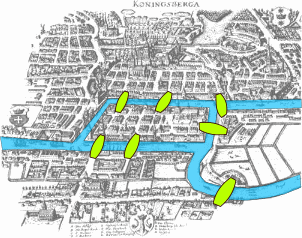
\includegraphics[scale=0.7]{Konigsberg_bridges}
	\caption[]{Representació dels ponts de Köingsberg \footnotemark}
	\label{fig:Königberg}	
\end{figure}
\footnotetext{Autor: Bogdan Giu\c{s}c\u{a}. Imatge de domini públic sota la llicència CC BY-SA 3.0 i GNU Free Documentation License (versió 1.2)}

Per aconseguir demostrar que el problema no tenia sol·lució, Euler va haver de representar el problema mitjançant un mapa topològic, posant les masses
de terra com a punts i els ponts com a segments que unien aquests
punts, i creant d'aquesta manera el primer graf de la història. Euler va observar que, exceptuant el punt inicial i final del trajecte, quan s'arriba a un punt per un pont, s'ha de sortir per un altre. Això significa que el nombre de vegades que s'entra a un punt equival al nombre de vegades que cal sortir-ne (exceptuant, tal com s'ha dit abans, el punt inicial i final), cosa que no és possible si no hi ha un nombre parell de ponts que vagin a un punt. Cal observar que en el problema original hi ha 4 masses de terra, i totes elles tenen un nombre imparell de ponts o arestes, i per tant no és possible passar per tots els ponts tan sols una vegada. Euler va arribar a la conclusió de que es pot recòrrer un graf passant només una vegada per les seves arestes només si aquest tenia 0 o 2 arestes de grau senar, que són les que anirien al punt final i inicial. 
Aquest resultat es considera el primer en teoria de grafs ja que conté un important teorema d'aquesta branca. A més d'iniciar la teoria de grafs, amb aquest resultat també comença l'estudi dels grafs planars, introdueix el concepte de característica d'Euler de l'espai i el teorema de poliedres d'Euler (teorema que després va utilitzar per demostrar que els sòlids platònics eren els únics sòlids regulars). Amb tot això, Euler posa les bases, no tan sols de l'estudi dels grafs, sinó també de la topologia. 

\begin{figure}[H]
\centering
\begin{tikzpicture}[scale=0.75,transform shape]
  \Vertex[x=0,y=0]0
  \Vertex[x=0,y=2]1
  \Vertex[x=0,y=4]2
  \Vertex[x=5,y=2]3
  \tikzstyle{LabelStyle}=[fill=white,sloped]
  \Edge(1)(3)
  \tikzstyle{EdgeStyle}=[bend left]
  \Edge(0)(1)
  \Edge(1)(2)
  \Edge(2)(3)
  \tikzstyle{EdgeStyle}=[bend right]
  \Edge(0)(1)
  \Edge(1)(2)
  \Edge(0)(3)
\end{tikzpicture}
\caption{Representació topològica dels ponts de Königsberg}
\end{figure}



\subsubsection*{Vandermonde i el tour del cavall d'escacs}

A partir de l'article d'Euler, diversos matemàtics van començar a
interessar-se pel camp de la topologia (o geometria de la posició,
com li deien en aquell moment). Un d'ells fou Alexandre-Théophile Vandermonde. Vandermonde va treballar i estudiar el problema dels cavalls, que planteja quins moviments hem de fer per tal que un cavall passi per totes les caselles del tauler d'escacs, problema que també va tractar Euler. Els estudis que Vandermonde va fer sobre aquest problema van ser publicats el 1771 en el ``\emph{Remarques sur des problèmes de situation''}, veure \cite{VAN71}, on encara no es feia referència al concepte de graf, tot i que el problema es resol mitjançant aquests. Aquest treball inicia l'estudi de la teoria de nusos, una altra branca de la topologia. 


\subsection{Les primeres descobertes i aplicacions}

Un cop establert l'inici, és difícil veure com va continuar desesenvolupant-se la teoria, ja que en els primers treballs es volien resoldre problemes concrets sense establir relacions entre ells. Tot i així, durant el segle XIX es van plantejar una gran qüantitat de problemes i es van desenvolupar molts teoremes referents als grafs.


\subsubsection*{Francis Guthrie}
\label{sec:Guthrie}
El 1852, Francis Guthrie, matemàtic britànic, es planteja el següent problema mentre intenta pintar un mapa del Regne Unit:
\begin{quote}
\emph{``És possible pintar qualsevol mapa de països de tal manera
que un país tingui un color diferent al de tots els seus veïns, utilitzant
tan sols quatre colors?''}
\end{quote}
D'aquest problema en surt el teorema a partir del qual s'sestableix que qualsevol mapa pot ser pintat únicament amb quatre colors diferents, de tal manera que dues regions adjacents (entenem com a adjacents dues regions que comparteixiin frontera, no tan sols un punt) no tinguin colors iguals. Aquest problema, que pot semblar tan trivial, no va ser demostrat fins l'any 1976. Va passar
per mans de pioners com De Morgan, Hamilton, Cayley, Kempe (que
va fer una demostració publicada el 1879, veure \cite{KEM79}), Heawood (que va concloure que la demostració de Kempe no era correcta)... Finalment el 1976
Appel i Hanken van demostrar, mitjançant un programa d'ordinador, que
tot mapa es podia pintar només amb quatre colors. Aquesta demostració i queda recollida a \cite{AH77a, AH77b}. Pel fet de basar-se en un programa d'ordinador, no va acabar de convèncer la demostració. Així doncs, aquest problema no va ser solucionat de manera formal fins l'any 1996 quan, recorrent a la teoria de grafs ja desenvolupada, Neil Robertson, Daniel P. Anders, Paul Seymour i Robin Thomas van publicar-ne una demostració. En els treballs d'Appel i Hanken es van definir alguns dels conceptes i fonaments de l'actual teoria de grafs. 


\subsubsection*{Arthur Cayley}

Arthur Cayley, matemàtic que treballava en la teoria de grups, topologia
i combintòria, també va aportar una gran quantitat de coneixement a la teoria de grafs. Va treballar amb grafs de tipus arbre i va desenvolupar
la fòrmula $n^{n-2}$, que determina el nombre d'arbres expansius
que té un graf complet de $n$ vèrtex (veure apartat \ref{sec:Complets}). Una fórmula semblant apareixia
en treballs de Carl Wilhelm Borchardt, en els quals Cayley es va basar
i va extendre, tot i que, actualment, qui dóna nom a la fórmula és el
mateix Cayley. 

També va treballar en el desenvolupament d'una representació de l'estructura
abstracta d'un grup, creant els grafs de Cayley i el teorema de Cayley. Finalment va contribuir també, l'any 1857, en la representació i ennumeració dels isòmers alcans (composts químics que comparteixen fórmula o composició però tenen diferent estructura molecular), representant cada compost mitjançant un graf de tipus arbre. Tot i això, Cayley no només va ser actiu en teoria de grafs, sinó que també va desenvolupar teoremes en àlgebra lineal, topologia i geometria.


\subsubsection*{William Hamilton i Thomas Kirkman }

William Rowan Hamilton va plantejar, l'any 1859, un problema que consistia
a trobar un camí que passés una sola vegada per cadascun dels 20 vèrtexs d'un dodecàedre tot recorrent les seves arestes. Hamilton el va comercialitzar
com a joc sota el nom de ``The Icosian game'' (és important dir que
el nom de icosian no feia referència a la utilització d'un icosaedre, sinó als 20 vèrtexs del dodecaedre per on s'havia de passar). Entorn aquest joc existeix un gran controvèrsia, ja que Euler anteriorment havia plantejat un problema semblant mentre estudiava el problema dels cavalls d'escacs, i Kirkman va plantejar a la Royal Society exactament el mateix problema que Hamilton un temps abans. 


\subsubsection*{Gustav Kirchhoff}

Gustav Kirchhoff, conegut majoritàriament en el camp de l'electrotècnia
per les lleis de Kirchhoff, també va fer aportacions importants
a la teoria de grafs. Les seves lleis, publicades el 1874, es basen
en la teoria de grafs, però a més, va ser el primer d'utilitzar els
grafs en aplicacions industrials. Va estudiar sobretot els grafs de
tipus arbre i, amb la investigació que va dur a terme, va formular el teorema de Kirchhoff, referent al nombre d'arbres d'expansió que es poden trobar en un graf. Aquest teorema es considera una generalització de la fórmula de Cayley.


\subsection{Teoria de grafs moderna}

Durant el segle XX, la teoria de grafs es va continuar desenvolupant.
Amb les bases ja establertes durant el segle XIX, els matemàtics hi
van començar a treballar i el 1936 Dénes König va escriure el primer
llibre de teoria de grafs: Theorie der endlichen und unendlichen Graphen (veure \cite{KON36}). Frank Harary va escriure el llibre "Graph Theory"
l'any 1969 (veure \cite{HAR69}), fent més accessible la teoria de grafs. El desenvolupament de la informàtica i les noves tècniques de computació van permetre treballar amb grafs a molt més gran escala, fent possible, per exemple, la ja citada primera demostració del teorema dels quatre colors per Appel i Hanken. 

Actualment la teoria de grafs és una part molt important de la matemàtica
discreta i està relacionada amb molts àmbits diferents, com per exemple
la topologia, la combinatòria, la teoria de grups, la geometria algebraica...
Des del seu desenvolupament s'han utilitzat els grafs per resoldre problemes referents a aquests camps i representar-los visualment. Té aplicacions
en molts altres àmbits com per exemple la computació, la informàtica,
la física, la química, l'electrònica, les telecomunicacions, la biologia,
la logística i fins i tot en l'àmbit econòmic. 

\section{Principis bàsics}

Un \textit{graf} $G=(V,E)$ es defineix com un conjunt de \textit{vèrtexs} (o nodes)
$V=\{v_{1},v_{2},...,v_{n}\}$ i un conjunt d'\textit{arestes} $E=\{e_{1},e_{2},...,e_{m}\}$, cadascuna de les quals uneix dos vèrtex de $V$. Si $v_{i}$ i $v_{j}$, amb $v_{i},v_{j}\in V$, estan units per l'aresta $e_{k}$ escriurem $e_{k}=\{v_{i},v_{j}\}$. Quan volguem especificar el graf concret empararem les notacions $V(G)$ i $E(G)$.
Així doncs un graf està format per un conjunt de punts i un conjunt
d'arestes que uneixen alguns d'aquests punts. El nombre de vèrtexs
d'un graf queda determinat pel nombre d'elements que hi ha en el conjunt
$V$, per tant ens referirem a ell com a $|V|$ (cardinal de $V$).
Amb les arestes passa el mateix, i també utilitzarem $|E|$ per indicar
el nombre d'arestes d'un graf. Definim també que dos vèrtexs són \textit{adjacents} si estan units per una aresta i, com a conseqüència, són \textit{incidents} a l'aresta. 
\\
La idea intuitiva de graf convida a utilitzar representacions gràfiques. Així, en la figura \ref{fig:exemple} es mostra un graf simple $G$ format
per:
\begin{itemize}
\item $V=\{v_{1},v_{2},v_{3},v_{4},v_{5},v_{6}\}$
\item $E=\{\{v_{1},v_{2}\},\{v_{1},v_{4}\},\{v_{1},v_{5}\},\{v_{2},v_{5}\},\{v_{3},v_{4}\},\{v_{3},v_{5}\},\{v_{3},v_{6}\},\{v_{4},v_{6}\}\}$


\end{itemize}

\begin{figure}[H]
\centering
	\begin{tikzpicture}[round/.style={circle, draw=black, thin, minimum size=2mm}, transform shape]
		\node[round] (a) at (0,4) {$v_{1}$};
		\node[round] (b) at (0,0) {$v_{2}$};
		\node[round] (c) at (4,0) {$v_{3}$};
		\node[round] (d) at (4,4) {$v_{4}$};
		\node[round] (e) at (2,2) {$v_{5}$};
		\node[round] (f) at (6,2) {$v_{6}$};
		\draw (a) edge (b);
		\draw (a) edge (d);
		\draw (a) edge (e);
		\draw (b) edge (e);
		\draw (c) edge (d);
		\draw (c) edge (e);
		\draw (c) edge (f);
		\draw (d) edge (f);
	\end{tikzpicture}
\caption{Representació gràfica del graf $G=(V,E)$ que s'ha presentat}
\label{fig:exemple}
\end{figure}


Si una aresta comença i acaba en el mateix vèrtex (per exemple $e_{m}=\{v_{i},v_{i}\}$
s'anomena llaç (figura \ref{fig:exemples_tipus}, cas (a)). També pot ser que hi hagi dues arestes idèntiques,
és a dir, dues arestes que uneixin $v_{i}$ i $v_{j}$ (figura \ref{fig:exemples_tipus}, cas (b)). En qualsevol d'aquests dos casos anteriors,
el graf s'anomena \textit{multigraf} o \textit{pseudograf}. En cas contrari, el graf
serà anomenat \textit{simple}. Amb el que hem vist fins ara, podem dir que
$e_{1}=\{v_{1},v_{2}\}$ és equivalent a $e_{2}=\{v_{2},v_{1}\}$, ja que es tracta de parells no ordenats. Tanmateix, existeixen grafs en els quals les arestes han de ser recorregudes en un sentit determinat. En aquest cas, s'anomenen grafs \textit{dirigits}. Aleshores si $e_{1}=(v_{1},v_{2})$ i $e_{2}=(v_{2},v_{1})$, $e_{1}\neq e_{2}$, ja que es tracta de parells ordenats (figura \ref{fig:exemples_tipus}, cas (c)). En la següent imatge
es mostren els grafs esmentats anteriorment:


\begin{figure}[H]
\centering
	\subfloat[]{
		\begin{tikzpicture}[round/.style={circle, draw=black, fill=black, thin, minimum size=1mm}, transform shape]
			\node[round] (a) at (0,0){};
			\node[round] (b) at (0,2) {};
			\node[round] (c) at (2,0) {};
			\node[round] (d) at (2,2) {};
			\draw (a) edge (b);
			\draw (a) edge (c);
			\draw (b) edge (d);
			\draw (d) edge (c);
			\draw (a) edge [looop] (a);

		\end{tikzpicture}
	}
	\subfloat[]{
		\begin{tikzpicture}[round/.style={circle, draw=black, fill=black, thin, minimum size=1mm}, transform shape]
			\node[round] (a) at (0,0){};
			\node[round] (b) at (0,2) {};
			\node[round] (c) at (2,0) {};
			\node[round] (d) at (2,2) {};
			\draw (a) edge [bend left](b);
			\draw (a) edge [bend right](b);
			\draw (a) edge [bend left](c);
			\draw (a) edge [bend right](c);
			\draw (b) edge (d);
			\draw (d) edge (c);
		\end{tikzpicture}
	}
	\subfloat[]{
		\begin{tikzpicture}[round/.style={circle, draw=black, fill=black, thin, minimum size=1mm}, transform shape]
			\node[round] (a) at (0,0){};
			\node[round] (b) at (0,2) {};
			\node[round] (c) at (2,0) {};
			\node[round] (d) at (2,2) {};
			\draw (a) edge[->, -Latex] (b);
			\draw (c) edge[->, -Latex] (a);
			\draw (b) edge[->, -Latex] (d);
			\draw (c) edge[->, -Latex] (d);
		\end{tikzpicture}
	}
\caption{Graf amb un llaç (a), graf amb arestes múltiples (b) i graf dirigit (c)}
\label{fig:exemples_tipus}
\end{figure}


Direm que un graf no dirigit $G=(V,E)$ és \textit{connex} si per a qualsevol $v_{i}, v_{j}\in V$ $v_{i}\neq v_{j}$ existeix un \textit{camí} (successió d'arestes) que els uneix.
\\
El nombre d'arestes que són incidents a un vèrtex $v$ (comptant els
llaços com a dues arestes) determinen el que anomenarem \textit{grau} de $v$, que es representa
amb $g(v)$. La successió de graus d'un graf serà la successió que
s'obté a l'ordenar de manera creixent els graus dels seus vèrtex. Cal
dir que no és un problema gens trivial saber si una successió de nombres naturals donada
pot ser una successió de graus d'un graf. El grau mínim d'un graf
$G=(V,E)$ queda determinat de la següent manera: $\delta(G)=min\{g(v):v\text{\ensuremath{\in}}V(G)\}$.
De manera similar, el grau màxim de $G$, $\text{\ensuremath{\Delta}}(G)=max\{g(v):v\text{\ensuremath{\in}}V(G)\}$.
\\
Si d'un graf connex en treiem una aresta o un node, en resulta un altre (o
més d'un) graf connex. Si $v\text{\ensuremath{\in}}V(G)$, indicarem per
$G-v$ al graf que s'obté al suprimir el vèrtex $v$ i totes les
seves arestes incidents. De la mateixa manera, si $e\text{\ensuremath{\in}}E(G)$,
$G-e$ indicarà el graf que s'obté a l'eliminiar la aresta $e$.

Amb tots aquests conceptes ja podem veure el teorema d'Euler, un dels
primers teoremes en teoria de grafs i un dels més importants.
\\
\\

\subparagraph{Teorema 1 (Euler)}
\label{teorema:Euler}
\begin{quotation}
En tot graf $G=(V,E)$, la suma dels graus dels vèrtex és igual al doble del
nombre d'arestes.\[ \sum_{v\in V(G)}g(v)=2|E(G)| \]
\end{quotation}
\emph{Demostració}: Només cal veure que cada aresta té dos extrems
i que suma dos en el total dels graus. La demostració formal és més
complicada, i comporta desenvolupar una inducció respecte del nombre d'arestes:

\begin{itemize}


\item Si $|E|=0$, no cal considerar el cas. Si $|E|=1$, o bé $|V|=2$ i cada
vèrtex té grau 1 o bé la aresta és un llaç i hi ha un sol vèrtex de grau
2. En qualsevol d'aquests dos casos, el teorema es verifica.
\item Ara suposem que el teorema està demostrat per a $|E|\leq k$ i que $G$ és un
graf amb $|E|=k+1$. Si $e$ és una aresta de $G$ prenem $H=G-e$.
\item Llavors tots els vèrtexs de $H$ tenen el mateix grau a $H$ que a
$G$ excepte 2 que tenen un grau menys o un que té dos graus menys
(només en el cas que $e$ sigués un llaç). En tots dos casos obtenim
que:\[ \sum_{v\in V(G)}g(v)=\sum_{v\in V(H)}g(v)+2=2(|E|-1)+2=2|E| \]D'aquesta
demostració en treiem una altra afirmació:

\end{itemize}

\begin{quotation}
\emph{En tot graf, el nombre de vèrtex amb grau imparell, és parell.}
\end{quotation}

\section{Isomorfismes}
Es diu que dos grafs són isomorfs si existeix una funció bijectiva $\varphi$ entre els seus vèrtexs que conservi les arestes. Formalment dos grafs $G$ i $H$ són isomorfs si

\[\exists\varphi:V(G)\rightarrow V(H) \text{ tal que } \forall u, v \in V(G)\text{, } \overline{\varphi(v)\varphi(u)}\in E(H) \text{ si i només si } \overline{vu}\in E(G)\]

\begin{figure}[H]
\centering
	\subfloat{
		\begin{tikzpicture}[round/.style={circle, text=white, thin, minimum size=.5mm}, transform shape, scale=0.80]
			\node[round, fill=blue] (a) at (0,0){2};
			\node[round, fill=red] (b) at (4,0){0};
			\node[round, fill=green] (c) at (2,1.5){3};
			\node[round, fill=purple] (d) at (2,4){1};
			\draw (a) edge (b);
			\draw (a) edge (c);
			\draw (a) edge (d);
			\draw (b) edge (c);
			\draw (b) edge (d);
			\draw (c) edge (d);
		\end{tikzpicture}
	}
	\subfloat{
		\begin{tikzpicture}[round/.style={circle, text=white, thin, minimum size=.5mm}, transform shape, scale=0.80]
			\node[round, fill=blue] (a) at (0,0){c};
			\node[round, fill=red] (b) at (4,0){a};
			\node[round, fill=green] (c) at (0,4){d};
			\node[round, fill=purple] (d) at (4,4){b};
			\draw (a) edge (b);
			\draw (a) edge (c);
			\draw (a) edge (d);
			\draw (b) edge (c);
			\draw (b) edge (d);
			\draw (c) edge (d);
		\end{tikzpicture}
	}
	\caption{Grafs isomorfs}
\end{figure}


\section{Tipus de grafs}
\label{Sec:tipus}

Fins ara hem vist els conceptes bàsics en teoria de grafs i algunes
de les propietats que compleixen tots els grafs. No obstant, existeixen
diversos tipus de grafs que tenen propietats especials. A continuació se'n presenten alguns.

\subsection{Graf lineal}
\label{sec:lineal}
Un graf lineal $L(G)$ d'un graf $G$ és un graf que representa les
adjacències entre les arestes de $G$. Formalment, donat un graf $G$,
el graf lineal $L(G)$ és aquell en el qual cada vèrtex correspon
a una aresta de $G$ i dos vèrtexs són adjacents només si les arestes
corresponents a $G$ comparteixen un vèrtex.

\begin{propietat}
El graf lineal d'un graf amb $n$ nodes, $e$ arestes i amb vèrtexs de graus
$g(v_{i})$ té $n'=e$ nodes i $e'$ arestes, on \[ e'=\frac{1}{2} \sum_{i=1}^{n}g(v_{i})^{2}-e \]
\\
\emph{Demostració}: Cada node $v_{i}$ amb grau $g(v_{i})$ del graf original generarà un graf complet de $g(v_{i})$ nodes ($K_{g(v_{i})}$) \footnote{Veure apartat \ref{sec:Complets}}.

	\begin{figure}[H]
		\centering
		\begin{tikzpicture}[round/.style={circle, draw=black, thin, minimum size=.5mm}, invisible/.style={shape=coordinate}, transform shape, scale=0.5]
			\node (a)[invisible] at (0,0){};
			\node (k)[invisible] at (14,0){};

			\node (g)[invisible] at (0,0.5){};
			\node (h)[invisible] at (3.5,0.5){};
			\node (i)[invisible] at (6.75,0.5){};
			\node (j)[invisible] at (14,0.5){};
			
			\node (b)[round] at (0, 6){$v_{i}$};

			\node (c) at (0,3){$w_{i_{0}}$};
			\node (d) at (2.5,2){$w_{i_{1}}$};
			\node (e) at (5,2){$w_{i_{2}}$};
			\node (f) at (7.5,3){$w_{i_{g(v_{i})}}$};
			
			\draw (b) edge (c);
			\draw (b) edge (d);
			\draw (b) edge (e);
			\draw (b) edge (f);
			\draw (c) edge (g);
			\draw (d) edge (h);
			\draw (e) edge (i);
			\draw (f) edge (j);
						
			\draw (c) edge[dashed] (d);
			\draw (c) edge[dashed] (e);
			\draw (c) edge[dashed] (f);
			\draw (d) edge[dashed] (e);
			\draw (d) edge[dashed] (f);
			\draw (e) edge[dashed] (f);
			
			\tikzset{doble/.style={<->,dashed}}
			\draw (a) edge[doble] node[midway,below]{$g(v_{i})$}(k);
						
		\end{tikzpicture}
	\end{figure}


Un graf complet té ${n\choose k} = \frac{n(n-1)}{2}$ arestes, per tant en aquest cas se'n generen $\frac{g(v_{i})(g(v_{i})-1)}{2}$. Però això es compleix per a cada vèrtex, i llavors podem escriure \[ \sum_{i=1}^{n}\frac{1}{2}g(v_{i})(g(v_{i})-1) = \frac{1}{2}\sum_{i=1}^{n}(g(v_{i})^{2}-g(v_{i})) = \frac{1}{2}\sum_{i=1}^{n}g(v_{i})^{2} - \underbracket{\frac{1}{2}\underbracket{\sum_{i=0}^{n}g(v_{i})}_{2|E|}}_{|E|} = \frac{1}{2}\sum_{i=1}^{n}g(v_{i})^{2}-e\]
\end{propietat}
\begin{figure}[H]
\centering
	\subfloat[$G$]{
		\begin{tikzpicture}[round/.style={circle, draw=black, thin, minimum size=.5mm}, transform shape, scale=0.5]
			\node[round] (a) at (8,4){$v_{0}$};
			\node[round] (b) at (4,8){$v_{1}$};
			\node[round] (c) at (0,8){$v_{2}$};
			\node[round] (d) at (0,4){$v_{3}$};
			\node[round] (e) at (4,0){$v_{4}$};
			\draw (a) edge (b);
			\draw (a) edge (d);
			\draw (a) edge (e);
			\draw (b) edge (c);
			\draw (b) edge (d);
			\draw (d) edge (e);
		\end{tikzpicture}
	}
	\subfloat[$G+L(G)$]{
		\begin{tikzpicture}[round/.style={circle, draw=black, thin, minimum size=.5mm}, transform shape, scale=0.5]
			\node[round] (a) at (8,4){$v_{0}$};
			\node[round] (b) at (4,8){$v_{1}$};
			\node[round] (c) at (0,8){$v_{2}$};
			\node[round] (d) at (0,4){$v_{3}$};
			\node[round] (e) at (4,0){$v_{4}$};
			\node[draw, diamond] (f) at (6,6){$u_{0}$};
			\node[draw, diamond] (g) at (2,8){$u_{1}$};
			\node[draw, diamond] (h) at (2,6){$u_{2}$};
			\node[draw, diamond] (i) at (2,2){$u_{3}$};
			\node[draw, diamond] (j) at (6,2){$u_{4}$};
			\node[draw, diamond] (k) at (4,4){$u_{5}$};
			\draw (a) edge (f);
			\draw (a) edge (j);
			\draw (a) edge (k);
			\draw (f) edge (b);
			\draw (j) edge (e);
			\draw (k) edge (d);
			\draw (b) edge (g);
			\draw (g) edge (c);
			\draw (b) edge (h);
			\draw (h) edge (d);
			\draw (d) edge (i);
			\draw (i) edge (e);
			
			\draw (f) edge[dashed] (h);
			\draw (k) edge[dashed] (f);
			\draw (k) edge[dashed] (j);
			\draw (k) edge[dashed] (i);
			\draw (k) edge[dashed] (h);
			\draw (f) edge[dashed] (h);
			\draw (i) edge[dashed] (j);
			\draw (g) edge[dashed] (h);
			\draw (f) edge[dashed] (j);
			\draw (h) edge[dashed] (i);
			\draw (g) edge[dashed, bend left=75] (f);
			
		\end{tikzpicture}
	}
	\subfloat[$L(G)$]{
		\begin{tikzpicture}[round/.style={circle, draw=black, thin, minimum size=.5mm}, transform shape, scale=0.5]
			\node[draw, diamond] (f) at (6,6){$u_{0}$};
			\node[draw, diamond] (g) at (2,8){$u_{1}$};
			\node[draw, diamond] (h) at (2,6){$u_{2}$};
			\node[draw, diamond] (i) at (2,2){$u_{3}$};
			\node[draw, diamond] (j) at (6,2){$u_{4}$};
			\node[draw, diamond] (k) at (4,4){$u_{5}$};
			\draw (f) edge (h);
			\draw (k) edge (f);
			\draw (k) edge (j);
			\draw (k) edge (i);
			\draw (k) edge (h);
			\draw (f) edge (h);
			\draw (i) edge (j);
			\draw (g) edge (h);
			\draw (f) edge (j);
			\draw (h) edge (i);
			\draw (g) edge (f);
		\end{tikzpicture}
	}
\caption{Procés de construcció d'un graf lineal}
\end{figure}

\subsection{Cicles}
\label{sec:cicles}

Els \textit{cicles} són grafs 2-regulars\footnote{Veure apartat \ref{sec:regulars}} amb $n$ vèrtexs i $n$ arestes, i s'anomenen $C_{n}$.
 
\begin{propietat}
El graf lineal d'un cicle és ell mateix.
\end{propietat}

\begin{figure}[H]
\centering	
	\begin{tikzpicture}
		\grCycle[RA=2, prefix=v, Math=true]{9}
	\end{tikzpicture}
\caption{Cicle $C_{9}$}
\end{figure}

\subsection{Grafs complets}
\label{sec:Complets}

Un \textit{graf complet} és un graf on cada vèrtex està unit a tots els altres
una sola vegada. Un graf complet amb $n$ nodes és un graf simple, $(n-1)$-regular i la seva nomenclatura és $K_{n}$. 

\begin{propietat}
Els grafs complets tenen ${n\choose 2}=\frac{n(n-1)}{2}$ arestes. 
\end{propietat}

\begin{propietat}
El nombre de cicles que conté un graf complet queda determinat per la següent igualtat:

\[ C_{n} =\sum_{K=3}^{n}\frac{1}{2}{n\choose k}(k-1)! \]

On:
\begin{description}
\item[$\frac{1}{2}$] es multiplica perquè es conten dues vegades els cicles, ja que no són dirigits.
\item[$n\choose k$] és el nombre de grups de $k$ elements que es poden agafar.
\item[$(k-1)!$] és el nombre de permutacions circulars de $k$ elements.
\end{description}

\end{propietat}

\begin{figure}[H]
\centering
	\subfloat[]{	
		\begin{tikzpicture}
			\grComplete[RA=2, prefix=v, Math=true]{7}
		\end{tikzpicture}
	}
	\subfloat[]{
		\begin{tikzpicture}
			\grComplete[RA=2, prefix=v, Math=true]{5}
		\end{tikzpicture}
	}
\caption{Grafs complets $K_{7}$(a) i $K_{5}$(b)}
\end{figure}

\subsection{Grafs bipartits}
\label{sec:bipartits}

Els \textit{grafs bipartits} són aquells en els quals els vèrtexs es poden
separar en dos conjunts disjunts $U$ i $W$ (és a dir, que els dos
conjunts no tinguin elements comuns) de tal manera que un vèrtex d'un
conjunt no sigui mai adjacent a un altre vèrtex del mateix conjunt.
Es pot dir també que un graf és bipartit si i sols si no conté cicles de longitud
senar. 

\begin{propietat}
Tots els grafs $C_{n}$ amb $n$ parell, són també grafs bipartits.
\end{propietat}

\begin{figure}[H]
\centering	
	\begin{tikzpicture}[v/.style={circle, fill=red, text=white, thin, minimum size=.5mm}, u/.style={circle, fill=blue, text=white, thin, minimum size=.5mm}, transform shape, scale=0.80]
		\node[v] (a) at (0,0){$v_{0}$};
		\node[v] (b) at (2,0){$v_{1}$};
		\node[v] (c) at (4,0){$v_{2}$};
		\node[v] (d) at (6,0){$v_{3}$};
		\node[u] (e) at (1,2){$u_{0}$};
		\node[u] (f) at (3,2){$u_{1}$};
		\node[u] (g) at (5,2){$u_{2}$};
		\draw (a) edge (e);
		\draw (b) edge (e);
		\draw (b) edge (f);
		\draw (b) edge (g);
		\draw (c) edge (e);
		\draw (c) edge (f);
		\draw (d) edge (f);
		\draw (d) edge (g);
	\end{tikzpicture}
\caption{Graf bipartit}
\end{figure}

\subsection{Grafs bipartits complets}
\label{sec:bipartits_complets}

Els \textit{grafs bipartits complets} són grafs bipartits en els quals cada
element del conjunt $U$ està unit a tots els elements dels del conjunt
$W$. S'anomenen $K_{m,n}$, on $m=|U|$ i $n=|W|$.

\begin{propietat}
En els grafs bipartits $K_{m,n}=K_{n,m}$ , $|V|=n+m$ i $|E|=mn$.
\end{propietat}

\begin{figure}[H]
\centering	
	\begin{tikzpicture}[v/.style={circle, fill=red, text=white, thin, minimum size=.5mm}, u/.style={circle, fill=blue, text=white, thin, minimum size=.5mm}, transform shape, scale=0.80]
		\node[v] (a) at (0,0){$v_{0}$};
		\node[v] (b) at (2,0){$v_{1}$};
		\node[v] (c) at (4,0){$v_{2}$};
		\node[v] (d) at (6,0){$v_{3}$};
		\node[v] (h) at (8,0){$v_{4}$};
		\node[u] (e) at (1,2){$u_{0}$};
		\node[u] (f) at (3,2){$u_{1}$};
		\node[u] (g) at (5,2){$u_{2}$};
		\node[u] (i) at (7,2){$u_{3}$};
		\draw (a) edge (e);
		\draw (a) edge (f);
		\draw (a) edge (g);
		\draw (a) edge (i);
		\draw (b) edge (e);
		\draw (b) edge (f);
		\draw (b) edge (g);
		\draw (b) edge (i);
		\draw (c) edge (e);
		\draw (c) edge (f);
		\draw (c) edge (g);
		\draw (c) edge (i);
		\draw (d) edge (e);
		\draw (d) edge (f);
		\draw (d) edge (g);
		\draw (d) edge (i);
		\draw (h) edge (e);
		\draw (h) edge (f);
		\draw (h) edge (g);
		\draw (h) edge (i);
	\end{tikzpicture}
\caption{Graf bipartit complet $K_{4,5}$}
\end{figure}

\subsection{Grafs xarxes}
\label{sec:xarxes}

Els \textit{grafs xarxes} bidimensionals $G_{m,n}$ són grafs bipartits que formen un entramat en forma de cuadrícula de $m\times n$ vèrtexs. 
\begin{propietat}
Es pot greneralitzar per a xarxes de més dimensions com a $G_{m,n,o,...}$. 
\end{propietat}
\begin{propietat}
Un graf xarxa té $mn$ vèrtexs i $(m-1)n+(n-1)m$ arestes. 

\emph{Demostració}: Tal com es pot veure a la figura \ref{fig:graus_xarxes}, un graf xarxa té 
\[
(n-2)(m-2)+2(m-2)+2(n-2)+4 = nm -\cancel{2m}-\cancel{2n}+\cancel{4}+\cancel{2m}-\cancel{4}+\cancel{2n}-\cancel{4}+\cancel{4} = mn
\] vèrtexs. D'altra banda, la suma dels graus de tots els vèrtexs és
\[
\frac{4(m-2)(n-2)+3\times 2(m-2+n-2)+4\times 2}{2} = 2(m-2)(n-2)+3(m-2)+3(n-2)+4
\]
Si es desenvolpua, s'obté
\[
(n-2)(m-2) + \important{(n-2)(m-2)+2(m-2)}+(m-2)+\important{2(n-2)}+(n-2)+\important{4}
\]
on la suma dels elements marcats equival a $mn$. Si es continua desenvolupant tenint en compte aquest detall, s'obté
\[
mn-2m-2n+4+m-2+n-2+mn = 2mn-m-n=\boxed{m(n-1)+n(m-1)}
\]

	\begin{figure}[H]
	\centering
		\begin{tikzpicture}[round/.style={circle, draw=black, fill=black, thin, minimum size=1mm}, invisible/.style={shape=coordinate}, central/.style={circle, draw=white, fill=white, thin, minimum size=1mm}, transform shape]
			\node (a)[round,label=grau 2] at (0,0){};
			\node (b)[round,label=grau 2] at (12,0){};
			\node (c)[round,label=grau 2] at (0,8){};
			\node (d)[round,label=grau 2] at (12,8){};
			\node (e)[invisible] at (1,0){};
			\node (f)[invisible] at (11,0){};
			\node (g)[invisible] at (0,1){};
			\node (h)[invisible] at (12,1){};
			\node (i)[invisible] at (0,7){};
			\node (j)[invisible] at (1,8){};
			\node (k)[invisible] at (11,8){};
			\node (l)[invisible] at (12,7){};
			\node (m)[invisible] at (1,1){};
			\node (n)[invisible] at (1,7){};
			\node (o)[invisible] at (11,1){};
			\node (p)[invisible] at (11,7){};
			\node (q)[central] at (6,4){grau 4};
			
			\draw (m) edge node [midway, fill=white]{\scriptsize{$n-2$}}(n);
			\draw (n) edge node [midway, fill=white]{\scriptsize{$m-2$}}(p);
			\draw (p) edge (o);
			\draw (o) edge (m);
			
			\draw (j) edge node [midway, fill=white, label={[yshift=0.01cm]\scriptsize{grau 3}}]{\scriptsize{$m-2$}}(k);
			\draw (e) edge node [midway, fill=white, label={[yshift=0.01cm]\scriptsize{grau 3}}]{\scriptsize{$m-2$}}(f);
			\draw (g) edge node [midway, fill=white, label={[xshift=-1cm, yshift=0cm]\scriptsize{grau 3}}]{\scriptsize{$n-2$}}(i);
			\draw (h) edge node [midway, fill=white, label={[xshift=1cm, yshift=0cm]\scriptsize{grau 3}}]{\scriptsize{$n-2$}}(l);
		
			

		\end{tikzpicture}
		\caption{Representació dels graus dels diferents nodes d'un graf xarxa}
		\label{fig:graus_xarxes}
	\end{figure}



\end{propietat}


\begin{figure}[H]
\centering
	\begin{tikzpicture}[round/.style={circle, draw=black, thin, minimum 			size=.5mm}, transform shape, scale=0.80]
		\node[round] (a) at (0,0){$v_{0}$};
		\node[round] (b) at (4,0){$v_{1}$};
		\node[round] (c) at (8,0){$v_{2}$};
		\node[round] (d) at (0,2){$v_{3}$};
		\node[round] (e) at (4,2){$v_{4}$};
		\node[round] (f) at (8,2){$v_{5}$};
		\node[round] (g) at (0,4){$v_{6}$};
		\node[round] (h) at (4,4){$v_{7}$};
		\node[round] (i) at (8,4){$v_{8}$};
		\draw (a) edge (b);
		\draw (a) edge (d);
		\draw (b) edge (c);
		\draw (b) edge (e);
		\draw (c) edge (f);
		\draw (d) edge (e);
		\draw (d) edge (g);
		\draw (e) edge (h);
		\draw (e) edge (f);
		\draw (f) edge (i);
		\draw (h) edge (i);
		\draw (h) edge (g);
	\end{tikzpicture}
\caption{Graf xarxa $G_{3,3}$}
\end{figure}

\subsection{Arbres}
\label{sec:arbres}

Els \textit{arbres} són un tipus molt important de grafs: són grafs connexos
sense cicles, de manera que existeix un únic camí entre dos vèrtexs.
\begin{propietat}
Si a un arbre se li afegeix una aresta, es genera un cicle, i si se'n
treu una, el graf deixa de ser connex.
\end{propietat} 
\begin{propietat}
Hi ha un tipus especial d'arbres anomenats \textit{elementals o camins}, que són els arbres amb $|V|=1$, $|V|=2$ i en general tots aquells on $\delta=1$ i $\Delta=2$. S'anomenen $P_{n}$, on $n=|V|$.
També es pot pensar en grafs elementals com a $G_{n,1}$.
\end{propietat}


\begin{figure}[H]
\centering
	\subfloat[]{
		\begin{tikzpicture}[round/.style={circle, draw=black, thin, minimum 			size=.5mm}, transform shape, scale=0.80]
			\tikzstyle{level 1}=[level distance=15mm,sibling distance=35mm]
			\node(0)[round]{$v_{0}$}
				child{node[round]{$v_{1}$}
					child{node[round]{$v_{3}$}}}
				child{node[round]{$v_{2}$}
					child{node[round]{$v_{4}$}}
					child{node[round]{$v_{5}$}}
			};
		\end{tikzpicture}
	}
	\subfloat[]{
		\begin{tikzpicture}
			\grEmptyPath[RA=1, prefix=v, Math=true]{4}
			\EdgeInGraphLoop*{v}{4}
		\end{tikzpicture}	
	}
\caption{Arbre (a) i graf elemental $P_{4}$ (b)}
\end{figure} 


\subsubsection*{Teorema 2}
\begin{quote}
Un arbre amb $n$ nodes té $n-1$ arestes. 
\end{quote}
\emph{Demostració: }Si comprovem el cas on un arbre $T$ té $n=1$ vèrtexs, veiem que no té cap aresta, per tant el teorema es compleix. Si treiem una aresta de l'arbre, sorgiran 2 arbres més $T_{1}$ i $T_{2}$. Per hipòtesi, $T_{1}$ tindrà $v_{1}=|V(T_{1})|$ vèrtexs i $n_{1}-1=|E(T_{1})|$ arestes, i $T_{2}$ tindrà $n_{2}=|V(T_{2})|$ vèrtexs i $n_{2}-1=|E(T_{2})|$ arestes.  Llavors el nombre d'arestes de $T$ és $(n_{1}-1)+(n_{2}-1)+1 = (n_{1}+n_{2})-1$. Deduïm llavors que el nombre de nodes de $T$ és $n_{1}+n_{2}$. Dit d'una altra manera, $|E(T)|=|V(T)|-1$.

Com a conseqüència d'aquest teorema, en podem arribar a un altre:

\subsubsection*{Teorema 3}
\begin{quote}
En un arbre $T$ amb $|V|\geq 2$, hi ha com a mínim dos vèrtexs de grau 1 (anomenats fulles).
\end{quote}
\emph{Demostració: } Fem un raonament per reducció a l'absurd. Suposem que no es compleix el teorema que volem demostrar, és a dir, que $g(v_{i}) > 1$ per a tots els vèrtexs. Llavors es compleix que \[ \sum_{v\in V}g(v) > \sum_{v\in V}2 =2|V|\] Però això no és correcte, ja que, com a conseqüència del Teorema 1 i Teorema 2 podem dir que en un arbre \[\sum_{v\in V}g(v)=2|E|=2|V|-2\]  i estem dient que $2|V|-2\geq2|V|$. Amb això ja podem veure que necessitem treure com a mínim dos graus, però demostrem també que amb un sol node de grau 1 tampoc és suficient. \smallskip Suposem ara que l'arbre té un sol node tal que $g(v)=1$ i elsaltres tenencom a mínim grau 2. Llavors \[ 2|V|-2=\sum_{v\in V}g(v)=1+\sum_{\substack{v\in V\\\text{si }g(v)\neq 1}}g(v)\geq 1+\sum_{\substack{v\in V \\\text{si }g(v)\neq 1}}2=1+2(|V|-1)=2|V|-1 \] Ara estem dient que $2|V|-2 \geq 2|V|-1$, que torna a ser una contradicció. Sabem que si treiem un grau més, el teorema es complirà, i hem demostrat que el mínim nombre de vèrtexs de grau 1 és 2.

Hi ha una altra manera de demostrar-ho, més directa:
Suposem que a l'arbre hi ha $k$ vèrtex de grau $1$, i $|V|-k$ de grau $g(v_{i})\geq 2$. D'aquesta manera
\[
2|V|-2=\sum_{v\in V}g(v) \geq k+2(|V|-k)=2|V|-k
\]
Llavors podem dir que $-2 \geq -k$ i per tant $2 \leq k$.
\\\\
Hi ha un altre teorema que relaciona el nombre de fulles amb el grau màxim d'un arbre:

\subsubsection*{Teorema 4}
\begin{quote}
El nombre de fulles d'un arbre $T$ és més gran o igual a $\Delta$.
\end{quote}
\emph{Demostració: }Si eliminem un node de grau $\Delta$ de l'arbre, juntament amb totes les seves arestes incidents, obtenim un conjunt de $\Delta$ grafs disconnexos. Si alguns d'aquests grafs consisteixen en tan sols un node, vol dir que abans eren adjacents al node que hem eliminat, per tant, només tenien grau 1. Si, pel contrari, formen nous arbres, pel teorema 3 podem dir que hi haurà com a mínim dues fulles. Encara que hi ha la possibilitat que un dels nodes amb grau 1 sigués l'adjacent al node que hem tret, sempre podem garantir que hi ha com a mínim una fulla. Per tant, també podem garantir que que hi haurà com a mínim $\Delta$ fulles.



\subsection{Graf roda}
\label{sec:rodes}

Un \textit{graf roda} amb $n$ vèrtex ès un graf que conté un cicle de longitud $n-1$, on tots els vèrtex del cicle estan connectats a un vèrtex fora del cicle, anomenat \textit{node central}. S'escriu $W_{n}$ i, a vegades, simplement s'estudia com a $C_{n-1}+K_{1}$. 

\begin{propietat}
El node central té grau $n-1$, i la resta de nodes tenen grau $3$.
\end{propietat}
\begin{propietat}
El nombre de cicles que conté un graf roda amb $n$ vètexs està determinat per $n^{2}-3n+3$.
\\
\emph{Demostració}: El nombre de cicles que conté un graf roda és la suma del nombre de cicles de longitud des de 3 fins a $n$ ($\sum_{i=3}^{n}C_{i}$). Amb l'exepció de $C_{n-1}$, el nombre de cicles per a cada $i$ és $n-1$. En el cas de $C_{n-1}$ n'hi ha $n$ de possibles, però ho representem de la manera $n-1+1$, per tal que sigui més còmode operar. Com que els cicles són possibles a partir de longitud 3, en total hi ha $n-2$ longituds possibles. D'aquesta manera podem escriure $(n-2)(n-1)+1=\boxed{n^{2}-3n+3}$.  
\end{propietat}


\begin{figure}[H]
\centering
	\begin{tikzpicture}
		\grWheel[RA=2, prefix=v, Math=true]{10}
	\end{tikzpicture}
\caption{Roda $W_{10}$}
\end{figure}

\subsection{Grafs estrella}	
\label{sec:estrella}

Un \textit{graf estrella} de grau $n$ és aquell que conté un vèrtex amb grau $n-1$ i els
$n-1$ vèrtexs restants de grau 1.
La seva nomenclatura és $S_{n}$. 

\begin{propietat}
Són estrelles tots els grafs bipartits de la forma $K_{1,n-1}$ o $K_{n-1,1}$. 
\end{propietat}
\begin{propietat}
El graf lineal de $S_{n}$ és $K_{n-1}$.
\end{propietat}

\begin{figure}[H]
\centering
	\begin{tikzpicture}
		\grStar[RA=2, prefix=v, Math=true]{7}
	\end{tikzpicture}
\caption{Graf estrella $S_{7}$}
\end{figure}

\subsection{Grafs complementaris} 
\label{sec:complementaris}

El \textit{graf complementari} del graf $G$ és el graf $H$ amb els mateixos
vèrtexs que $G$, de manera que dos vèrtexs d'$H$ seran adjacents
si i només si a $G$ no ho són. Formalment, si $G=(V,E)$ és un graf
simple i $K=E(K_{n})$ és el conjunt d'arestes derivades de totes les possibles combinacions de
dos elements de $V$, essent $n=|V(G)|$, llavors $H=(V,K\setminus E)$    	\footnote{La notació $K\setminus E$ indica el conjunt dels elements de $K$ que no són a $E$}. 
Per indicar el complementari de $G$ s'escriu $\bar{G}$ o $G'$. 

\begin{propietat}
Per obtenir el graf complementari
de $G$ tan sols cal afegir les arestes que falten per obtenir
un graf complet i treure totes les que hi eren inicialment (ja que
$|E(G)|+|E(\bar{{G}})|=|K|$). Veure figura \ref{fig:complementari}.
\end{propietat}

\begin{figure}[H]
\centering
	\subfloat{
		\begin{tikzpicture}[scale=.5]
			\grCirculant[RA=3, prefix=v,Math=true]{6}{2,3}
		\end{tikzpicture}
	}
	\subfloat{
		\begin{tikzpicture}[scale=.5]
			\grCirculant[RA=3, prefix=v,Math=true]{6}{1}
		\end{tikzpicture}
	}
\caption{Un graf $G$ i el seu complementari $\bar{G}$}
\label{fig:complementari}
\end{figure}

\subsection{Graf nul i grafs buits}
\label{sec:buits}

Els \textit{grafs buits} són grafs sense arestes, és a dir, conjunts d'$n$ vértexs.
Són els complementaris dels grafs complets $K_{n}$, i per tant la seva nomenclatura
és $\bar{K}_{n}$, o simplement, $N_{n}$. Estrictament s'anomena \textit{graf nul} a $N_{0}$
i buits a la resta, però com que normalment no s'utilitza $N_{0}$,
convencionalment es diuen nuls tots els elements del conjunt dels buits.

\begin{figure}[H]
\centering
	\begin{tikzpicture}[round/.style={circle, draw=black, thin, minimum 			size=.5mm}, transform shape, scale=0.80]
		\node[round] (a) at (0,0){$v_{0}$};
		\node[round] (b) at (4,0){$v_{1}$};
		\node[round] (c) at (8,0){$v_{2}$};
		\node[round] (d) at (0,2){$v_{3}$};
		\node[round] (d) at (4,2){$v_{4}$};
		\node[round] (d) at (8,2){$v_{5}$};
	\end{tikzpicture}
\caption{Graf buit $N_{6}$}
\end{figure}

\subsection{Grafs regulars} 
\label{sec:regulars}

Es diu que un graf $G=(V,E)$ és \textit{regular de grau $r$} quan tots els seus vèrtexs
tenen grau $r$. Formalment, un graf és $r$-regular quan $\Delta(G)=\delta(G)=r$.
Un graf $0$-regular és un graf nul \footnote{Veure apartat \ref{sec:buits}}, un graf $1$-regular
consisteix en arestes separades entre elles i un graf $2$-regular
consisteix en un o més cicles separats. A partir d'aquí, els grafs regulars més importants
tenen noms propis, com per exemple els $3$-regulars, que són els
\textit{cúbics}; els $4$-regulars, \textit{quàrtics}; els $7$-regulars, \textit{grafs de Witt
truncats dobles}; els $8$-regulars, \textit{grafs de 24 cel·les}... 

A la imatge \ref{fig:regulars} es poden veure diversos exemples de grafs regulars.

\begin{propietat}
No necessàriament existeix un únic graf $r$-regular, sinó
que sovint s'en poden fer amb diferent nombre de vèrtexs.

\end{propietat}

\begin{propietat}
Com a conseqüència del teorema \ref{teorema:Euler}, per a tots els grafs $r$-regulars amb $n$ vèrtexs es compleix que 

\[ |E(G)|=\frac{1}{2}nr \]on $|E(G)|$ és el nombre d'arestes.
\end{propietat}

%Cal afegir imatges de més grafs 3-regulars.

\begin{figure}[H]
\centering
\subfloat[Graf cúbic (3-regular)]{
	\begin{tikzpicture}[round/.style={circle, draw=black, thin, minimum size=.5mm}, transform shape, scale=0.80]
		\node[round] (a) at (0,0){$v_{2}$};
		\node[round] (b) at (4,0){$v_{0}$};
		\node[round] (c) at (2,1.5){$v_{3}$};
		\node[round] (d) at (2,4){$v_{1}$};
		\draw (a) edge (b);
		\draw (a) edge (c);
		\draw (a) edge (d);
		\draw (b) edge (c);
		\draw (b) edge (d);
		\draw (c) edge (d);

	\end{tikzpicture}
	}
\subfloat[Graf 2-regular]{
	\begin{tikzpicture}[round/.style={circle, draw=black, thin, minimum size=.5mm}, transform shape, scale=0.80]
	
		\node[round] (0) at (3,1){$v_{0}$};
		\node[round] (1) at (3,3){$v_{1}$};
		\node[round] (2) at (1.5,4){$v_{2}$};
		\node[round] (3) at (0,3){$v_{3}$};
		\node[round] (4) at (0,1){$v_{4}$};
		\node[round] (5) at (1.5,0){$v_{5}$};
		
		\draw (0) edge (4);
		\draw (0) edge (5);
		\draw (4) edge (5);
		\draw (1) edge (2);
		\draw (1) edge (3);
		\draw (2) edge (3);
	\end{tikzpicture}
}
\subfloat[Graf 4-regular]{
	\begin{tikzpicture}[]
		\grEmptyCycle[RA=2, prefix=v, Math=true]{10}
		%\EdgeInGraphModLoop{v}{8}{2}{0}
		\EdgeFromOneToSel{v}{v}{0}{2,4,6,8}
		\EdgeFromOneToSel{v}{v}{1}{3,5,7,9}
		\EdgeFromOneToSel{v}{v}{2}{4,6,8}
		\EdgeFromOneToSel{v}{v}{3}{5,7,9}
		\EdgeFromOneToSel{v}{v}{4}{6,8}
		\EdgeFromOneToSel{v}{v}{5}{7,9}
 		\EdgeFromOneToSel{v}{v}{6}{8}
		\EdgeFromOneToSel{v}{v}{7}{9}	
	\end{tikzpicture}
}
\caption{Exemples de grafs regulars}
\label{fig:regulars}
\end{figure}






\newpage
\chapter{Camins i algorismes}

\begin{flushright}
\textit{"Simplicity is a prerequisite for reliability"}
\\Edsger W. Dijkstra
\end{flushright}

Sovint, quan utilitzem un graf per modelitzar quelcom, ens interessa
poder-hi fer algunes operacions. Podem, per exemple, voler trobar
un camí entre dos punts, recòrrer el graf sencer o trobar el camí
més curt per anar d'un vèrtex a un altre. Per aquest motiu utilitzem
els camins, que trobarem o generarem mitjançant diversos algorismes.

En aquesta secció es mostraran i s'implementaran diverses maneres de recòrrer un graf, trobant
la manera més eficient per a cada cas.

\section{Grafs ponderats i dirigits}
\subsection{Grafs ponderats}
Els \textit{grafs ponderats} són grafs on cada aresta $e$ està associada a un nombre $w(e)$ anomenat \textit{pes o cost}, tal que $w(e)\in \mathbb{R}$. El pes pot representar diverses quantitats, segons el que es vulgui modelitzar. 
Moltes vegades s'utilitza per representar distàncies, però si per exemple modelitzem una xarxa de distribució d'aigua, ens pot interessar representar el cabal de les canonades, o en una xarxa de bus, la densitat de trànsit de cada tram. 

\subsection*{Grafs dirigits}
Els \textit{grafs dirigits} són grafs les arestes dels quals només admeten un sentit. D'aquesta manera, una aresta $e_{0}=(v_{0},v_{1}) \neq e_{1}=(v_{1},v_{0})$ \footnote{Observi's la diferència de notació per a les arestes dels grafs dirigits i no dirigits, atenent al fet que l'ordre dels vèrtexs en un cas importa i en l'altre no}. De fet, no necessàriament ha d'existir una aresta contrària a una altra. 

Aquest tipus de grafs poden ser útils per representar carreteres, o moviments vàlids en algun joc. 


\section{Camins}

Un \textit{camí} $p$ és una seqüència finita i ordenada d'arestes que connecta
una seqüència ordenada de vèrtexs. Un camí $p$ de longitud $k$ (expressat com a $l(p)=k$) entre el vèrtex inicial $v_{0}$ i el vèrtex final $v_{k}$ (sempre que $v_{0}\neq v_{k}$) és una successió de $k$ arestes i $k+1$ vèrtexs de la forma $\overline{v_{0},v_{1}}, \overline{v_{1},v_{2}},\cdots, \overline{v_{k-1},v_{k}}$  . Per definició, també es pot representar un camí $p$ entre $v_{0}$ i $v_{k}$ com a successió de vèrtex $p=v_{0}v_{1}\cdots v_{k}$. En aquest cas, pot ser tractat com un graf elemental $P_{n}$. 

Un cas especial és quan el camí comença i acaba al mateix vèrtex ($v_{0} = v_{k}$). Llavors el camí és un cicle, i és l'equivalent a un graf cicle $C_{n}$. 

Quan un camí té totes les arestes diferents, s'anomena \textit{simple}, i si a més té tots els vèrtexs diferents, s'anomena \textit{elemental}.

En els grafs, ponderats, la \textit{longitud} d'un camí $p=v_{0}v_{1}\cdots v_{n}$ no es defineix pel nombre d'arestes per on passa el camí, sinó fent el sumatori dels pesos de les arestes
\[ \textbf{longitud}_{w}(c)=\sum_{i=0}^{n-1}w(\overline{v_{i},v_{i+1}}) \]

La \textit{distància} entre dos vèrtexs $v$ i $u$, $d_{w}(v,u)$, és la que s'obté a l'agafar la menor longitud d'entre tots els camins elementals entre $v$ i $u$. 

\subsection{Camins Eulerians}
Un \textit{camí Eulerià} d'un graf és un camí que recorre totes les arestes d'un graf una sola vegada. De la mateixa manera, un cicle Eulerià consisteix en un camí que utilitza totes les arestes d'un graf una sola vegada i el punt inicial i final és el mateix. 
Un graf connex té un camí Eulerià si i només si té $0$ o $2$ vèrtexs de grau imparell, i té un cicle Eulerià si i només sí tots els vèrtex del graf tenen grau parell.

\subsection{Camins Hamiltonians}
Un camí Hamiltonià és un camí que passa una sola vegada per cadascún dels vèrtexs d'un graf. Un cicle Hamiltonià és un camí Hamiltonià en el qual el vèrtex inicial és igual al vèrtex final.


\section{Estructures de dades dels grafs}

En els grafs, normalement s'ha de tractar una gran quantitat d'informació:
nodes, arestes, pesos, sentits... Tota aquesta informació no és difícil
de gestionar si el graf que s'estudia és petit, ja que fins i tot
es pot dibuixar. El problema sorgeix quan el graf en qüestió és més
gran, com per exemple podria ser una xarxa de clavagueram o de metro.
Llavors la informació a tractar és molta, i és convenient organitzar-la
en estructures de dades. Les estructures de dades solen ser utilitzades
en la programació, però en aquest cas sol ser beneficiós usar-ne
fins i tot quan no es treballa amb informàtica.

Les matrius i llistes d'adjacència són les més utilitzades.


\subsection*{Matrius}


\subsubsection*{Matriu d'adjacència}

La \textit{matriu d'adjacència} d'un graf és una matriu quadrada que conté
informació respecte el nombre d'arestes que uneixen qualsevol parella de nodes, i s'organitza
de la següent manera:

Si $G$ és un graf amb $|V|$ nodes, $A(G)=(a_{ij})_{ij=1,...,|V|}$
és la seva matriu d'adjacència de $|V|\times|V|$, on $a_{ij}$ correspon
al nombre d'arestes que uneixen els nodes $i$ i $j$, contant com a 2
els llaços, que sempre es trobaràn a la diagonal. La matriu serà simètrica
si el graf ho ès, i podrem conèixer el grau d'un node $i$ fent el sumatori de les caselles de la $i$-èsima fila. A vegades, quan s'utilitzen grafs ponderats, les matrius d'adjacència s'omplen amb els pesos de les arestes, per no haver d'utilitzar altres estructures per emmagatzemar la resta d'informació. En aquest tipus de grafs, els llaços no necessàriament valdran 2, però es podran diferenciar perquè estaràn a la diagonal. En aquest cas, el problema serà que no es podran representar arestes múltiples amb pesos diferents. Tot i així, en termes de programació, utilitzar aquesta estructura de dades (sobretot en grafs grans) no
és el més eficient, ja que la matriu creix molt ràpidament. La matriu d'un graf
de $|V|$ nodes té $|V|^{2}$ espais, i en grafs poc densos, la majoria
d'espais estan ocupats per $0$, de tal manera que s'està utilitzant
molta memòria que no conté informació útil. De la mateixa manera,
si afegim un nou node al graf, que serà l'$n$-èssim, s'haurà d'afegir
$2n-1$ espais a la matriu.




\subsubsection*{Matriu d'incidència}

La \textit{matriu d'incidència} d'un graf $G$ sense llaços, $I(G)=(b_{i,j})_{i=1,...,|V(G)|,j=1,...,|E(G)|}$, és la matriu binària de $|V(G)|\times |E(G)|$ on $b_{i,j}$
indica si l'aresta $j$ és incident al node $i$.

\begin{figure}[H]
\centering
	\subfloat[Graf G]{
		\begin{tikzpicture}[round/.style={circle, draw=black, thin, minimum size=.5mm}, transform shape, scale=0.80]
				\node[round] (a) at (4,0){$v_{0}$};
				\node[round] (b) at (2,4){$v_{1}$};
				\node[round] (c) at (0,0){$v_{2}$};
				\node[round] (d) at (2,0){$v_{3}$};
				\node[round] (e) at (2,2){$v_{4}$};
				\draw (a) edge (b);
				\draw (a) edge (d);
				\draw (b) edge (c);
				\draw (b) edge (e);
				\draw (c) edge (d);
				\draw (d) edge (e);	
	
		\end{tikzpicture}
	}
	\subfloat[A(G)]{
		$\begin{bmatrix}
			0 & 1 & 0 & 1 & 0 \\
			1 & 0 & 1 & 0 & 1 \\
			0 & 1 & 0 & 1 & 0 \\
			1 & 0 & 1 & 0 & 1 \\
			0 & 1 & 0 & 1 & 0
		\end{bmatrix}$
	}
	\subfloat[I(G)]{
		$\begin{bmatrix}
			1 & 0 & 1 & 0 & 0 & 0 \\
			1 & 1 & 0 & 1 & 0 & 0 \\
			0 & 1 & 0 & 0 & 1 & 0 \\
			0 & 0 & 1 & 0 & 1 & 1 \\
			0 & 0 & 0 & 1 & 0 & 1  
		\end{bmatrix}$	
	}
\caption{Graf G amb les seves corresponents matrius d'adjacència i incidència}

\end{figure}



\subsection*{Llistes d'adjacència}

Aquesta estructura de dades és molt utilitzada per tractar grafs,
ja que ocupa menys memòria i només inclou la informació necessària.
Les \textit{llistes d'adjacència} d'un graf $G$ consisteixen en un conjunt de $|V(G)|$ llistes.
Cada llista correspon a un node del graf, i conté els nodes al quals
és adjacent. En informàtica s'acostumen a fer mitjançant apuntadors,
de tal manera que, a partir de cada element de la llista, es pugui
accedir a la seva pròpia llista, essent així molt més eficient fer
iteracions. Amb l'esquema següent es pot veure més clarament:

\begin{figure}[H]
\setcounter{subfigure}{0}
\centering
\subfloat[]{
	\begin{tikzpicture}[round/.style={circle, draw=black, thin, minimum size=.5mm}, transform shape, scale=0.80]
				\node[round] (a) at (0,3){$v_{0}$};
				\node[round] (b) at (3,3){$v_{1}$};
				\node[round] (c) at (0,0){$v_{2}$};
				\node[round] (d) at (3,0){$v_{3}$};
				\node[round] (e) at (5,1.5){$v_{4}$};
				\draw (a) edge (b);
				\draw (b) edge (c);
				\draw (b) edge (d);
				\draw (b) edge (e);
				\draw (c) edge (d);
				\draw (c) edge (e);
	
		\end{tikzpicture}
}
\subfloat[]{
	\begin{tikzpicture}
		\foreach [count=\i] \index/\list in {$v_{0}$/{$v_{1}$}, $v_{1}$/{$v_{0}$,$v_{2}$,$v_{3}$,$v_{4}$}, $v_{2}$/{$v_{1}$,$v_{3}$,$v_{4}$}, $v_{3}$/{$v_{1}$, $v_{2}$}, $v_{4}$/{$v_{1}$,$v_{2}$}} {
    		\node[array element] (aux) at (0,-\i) {\index};
    		\LinkedList{\list}
}
	
	\end{tikzpicture}
}
\caption{Un graf $G$ (a) i la seva llista d'adjacència (b)}
\end{figure}


\section{Algorismes}
Un \textit{algorisme} és un conjunt d'instruccions precises i ben definides que, donada una entrada, calculen la sortida corresponent segons les instruccions que té.

Per automatitzar diversos càlculs sobre grafs, molts científics han treballat desenvolupant processos universals que poden ser duts a terme per ordinadors. Aquests processos, anomenats \emph{algorismes}, consisteixen en conjunts específics d'ordres que s'executen sobre unes estructures de dades que contenen el graf.   

Per fer l'anàlisi dels algorismes, s'haurà de fer l'anàlisi de la cota superior asimptòtica, és a dir, analitzar el temps d'execució de l'algorisme quan l'entrada és la més gran i complexa possible. Per a aquest propòsit s'utiltizarà la notació de Landau, també anomenada notació de la gran "O". Els temps majoritàriament es calcularan en funció del nombre d'arestes o de nodes. Cal tenir present que tots els logaritmes que apareguin en funcions de Landau són logaritmes en base 2, sempre que no s'indiqui el contrari.

A continuació se'n mostren uns quants d'importants per fer operacions sobre grafs.

\subsection{BFS}
Aquest algorisme serveix per examinar l'estructura d'un graf o fer-ne un recorregut sistemàtic. La recerca per amplada prioritària (\emph{breadht-first serch} en anglès, d'aquí \textbf{BFS}) fa l'exploració en paral·lel de totes les alternatives possibles per nivells des del vèrtex inicial. A la imatge \ref{fig:bfs} es pot veure com funcionaria aquest algorisme en un graf. 
Per programar aquest algorisme s'acotuma a utilitzar un contenidor de tipus cua, que només permet afegir elements al final de la cua i treure'n de l'inici, sense poder accedir a elements del mig.
El que farà el programa serà imprimir per pantalla la seqüència de vèrtexs ordenada segons l'ordre en que els ha visitat.   

\subsubsection{Funcionament}

Donat un node incial $v$, es busquen tots els nodes no visitats que estiguin a distància $i$ de $v$. Inicialment $i=0$ i l'únic a distància 0 de $v$ és ell mateix. Després, $i=1$ i per tant, en aquesta iteració es visitaran tots els nodes adjacents a $v$. Quan $i=2$ es visitaran els nodes adjacents als adjacents de $v$ que no s'hagin visitat, i així consecutivament fins a visitar tots els nodes.



\begin{figure}[H]
\centering
\begin{tikzpicture}[round/.style={circle, draw=black, black, thin, minimum size=.5mm}, transform shape, scale=0.80]
		\tikzstyle{level 1}=[level distance=15mm,sibling distance=60mm]
		\tikzstyle{level 2}=[level distance=15mm,sibling distance=30mm]
		\node(0)[round](0){$0$}
			child[blue,shift={(0,0)}]{node[round](1){$1$}
				child[green]{node[round](2){$2$}}
				child[green]{node[round](3){$3$}}
				child[green]{node[round](4){$4$}}}
			child[blue]{node[round](5){$5$}
				child[green]{node[round](6){$6$}
					child[red]{node[round](7){$7$}}}
				child[green]{node[round](8){$8$}}
			};
			
		\tikzset{dfs/.style={bend right=15}}
		\draw (0) edge[dfs,green] (1);
		\draw (0) edge[dfs,red] (5);
		\draw (5) edge[dfs,green] (0);
		\draw (5) edge[dfs,red] (6);		
		
	\end{tikzpicture}
\caption{Exemple del recorregut que realitzaria l'algorisme}
\label{fig:bfs}		

\end{figure}

\subsubsection{Pseudocodi}

\begin{algorisme}[H]
\DontPrintSemicolon
\KwData{Un graf $G$ i un node inicial $v$}
\KwResult{Seqüència de de nodes visitats}
nova cua Q\;
marca $v$ com a visitat\;
afegeix $v$ a la cua $Q$\;
nou node $auxiliar$\;
nou node $seg\ddot{u}ent$\;
\While{la cua no estigui buida}
{
	$auxiliar$ = primer element de $Q$\;
	imprimeix($auxiliar$)\;
	elimina(primer element de $Q$)\;
	
	\While{hi hagi nodes adjacents a $auxiliar$ i aquests no s'hagin visitat}
	 {
	 	marca adjacent($auxiliar$) com a visitat\;
	 	afegeix adjacent($auxiliar$) a la cua\; 
	 }
	   
}
\ForEach{node de $G$}{marca'l com a no visitat}
\caption{BFS}

\end{algorisme}

\leavevmode
\\\\
Aquesta és una manera bastant usual de programar l'algorisme BFS, i encara que és eficient, s'està desaprofitant propietats de l'algorisme. Amb l'algorisme BFS es pot saber a quina distància del punt inicial està cada node, el camí més curt per anar del node inicial a qualsevol altre i fins i tot es pot generar un arbre expansiu mínim, agafant les arestes per on 'passa' l'algorisme.
El següent algorisme té en compte aquests detalls. Està pensat per ser implementat en el llengüatge Python, i per aquest motiu utilitza diccionaris (llistes on cada element té una clau i un valor), però en llenguatges basats en C, es poden utilitzar "maps" de la mateixa manera.

\begin{algorisme}
\DontPrintSemicolon
\KwData{Un graf $G$ i un node inicial $v$}
\KwResult{Seqüència de nodes visitats, distància de cada node resperce $v$}
nou diccionari $dist$\;
$dist[v]=0$\;
nou diccionari $anterior$\;
$anterior[v]=Nul$\;
$i=0$\;
nova llista $frontera$
afegeix $v$ a $frontera$\;
imprimeix($v$)\;
\While{frontera no estigui buida}
{
	nova llista $seg\ddot{u}ent$\;
	\ForEach{node $x$ de $frontera$} 
	{
		\tcc{A cada iteració, $x$ agafarà un valor diferent de $frontera$} 
		\ForEach{node $y$ adjacent a $x$ }
		{
			\If{$y$ no existeix dins $dist$}
			{
				$dist[y]=i$\;
				$anterior[y]=x$\;
				afegeix $y$ a $seg\ddot{u}ent$\;
				imprimeix($y$)\;			
			}		
		}
	}
	$frontera=seg\ddot{u}ent$\;
	$i=i+1$\;
}
imprimeix($dist$)\;
\end{algorisme}

 

\subsubsection{Aplicacions}
Encara que aquest algorisme sembli molt senzill, ens pot aportar informació important, i fins i tot permet resoldre problemes senzills on haguem de trobar distàncies o el camí més curt entre dos nodes.
Aquest algorisme s'utilitza també per operacions més complexes, com les següents: 
\begin{itemize}

\item Buscadors com Google l'utilitzen per indexar pàgines web noves. Amb l'algorisme BFS pot recòrrer tota la xarxa d'internet sencera, i, si cada pàgina web és un node i cada enllaç és una aresta, si es posa un link d'una pàgina no indexada a una que sí ho està, l'algorisme trobarà el nou node.
\item Les xarxes socials l'utilitzen per suggerir amistats. Amb aquest algorisme es poden trobar els amics d'una persona (els nodes que estan a distància 2 d'aquesta), que són susceptibles a ser amics seus. Com més amistats en comú amb la persona a distància 2, més probable és que es coneguin. 
\item Es pot sol·lucionar un cub de rubik. Si s'aconsegueix generar un graf on cada node sigui un estat diferent del cub i les arestes siguin un moviment d'una cara, donat un estat inicial, amb BFS es pot arribar a l'estat resolt amb els mínims moviments possibles.

\end{itemize}
 

\subsection{DFS}
La recerca per profunditat prioritària (\emph{depth-first search} en anglès, d'aquí \textbf{DFS}) és un algorsime que utilitza uns principis semblants als de l'algorisme BFS, però en lloc de cobrir tota l'amplada d'un nivell abans de passar al següent, el que fa és cobrir tota la profunditat possible (arribar el més lluny possible) abans de tornar enrere.

\subsubsection{Funcionament}
L'algorisme DFS arriba el mes lluny possible abans de retrocedir. Això significa que quan arriba a un node se'n va a un d'adjacent no visitat i va emmagatzemant l'ordre amb el qual els visita. Quan un node no té nodes adjacents no visitats, torna al node anterior i continua a partir d'allà. 
A la figura \ref{fig:bfs} es mostra un graf amb els nodes numerats segons l'ordre en el qual es visiten i amb el recorregut que faria l'algorisme:

\begin{figure}[H]
\centering
\begin{tikzpicture}[round/.style={circle, draw=black, thin, minimum 			size=.5mm}, transform shape, scale=0.80]
		\tikzstyle{level 1}=[level distance=15mm,sibling distance=60mm]
		\tikzstyle{level 2}=[level distance=15mm,sibling distance=30mm]
		\node(0)[round](0){$0$}
			child{node[round](1){$1$}
				child{node[round](2){$2$}}
				child{node[round](3){$3$}}
				child{node[round](4){$4$}}}
			child{node[round](5){$5$}
				child{node[round](6){$6$}
					child{node[round](7){$7$}}}
				child{node[round](8){$8$}}
			};
			
		\tikzset{dfs/.style={red,dashed,->,bend right=25, -latex}}
		\draw (0) edge[dfs] (1);
		\draw (1) edge[dfs] (2);
		\draw (2) edge[dfs] (1);
		\draw (1) edge[dfs] (3);
		\draw (3) edge[dfs] (1);
		\draw (1) edge[dfs] (4);
		\draw (4) edge[dfs] (1);
		\draw (1) edge[dfs] (0);
		\draw (0) edge[dfs] (5);
		\draw (5) edge[dfs] (6);
		\draw (6) edge[dfs] (7);
		\draw (7) edge[dfs] (6);
		\draw (6) edge[dfs] (5);
		\draw (5) edge[dfs] (8);		
		
	\end{tikzpicture}
\caption{Exemple del recorregut que realitzaria l'algorisme}
\label{fig:dfs}		

\end{figure}
 
\subsubsection{Pseudocodi}

Tal com en el BFS, també hi ha diverses maneres d'implementar l'algorisme, i en presentaré dues. La primera utilitza un contenidor de tipus pila, on només es pot manipular, afegir o treure l'element de dalt de tot d'aquest. \\

\begin{algorisme}[H]
\DontPrintSemicolon
\KwData{Un graf $G$ i un node inicial $v$}
\KwResult{Seqüència de nodes visitats}
nova pila $S$\;
nou node $seg\ddot{u}ent$\;
marca $v$ com a visitat\;
imprimeix($v$)\;
afegeix $v$ a la pila $S$\;
\While{la pila no estigui buida}
{	
	$seg\ddot{u}ent=$ node adjacent no visitat de l'element superior de $S$\;
	\tcc{En cas que no n'hi hagi cap, $seg\ddot{u}ent=Nul$} 
	\uIf{$seg\ddot{u}ent=Nul$}
	{
		elimina(element superior de $S$)\;	
	}
	\Else
	{
		marca $seg\ddot{u}ent$ com a visitat\;
		imprimeix($seg\ddot{u}ent$)\;
		afegeix $seg\ddot{u}ent$ a $S$\; 
	}
}



\caption{DFS}
\end{algorisme}
\leavevmode
\\
Aquest métode, però, té un problema, i és que només funciona per a grafs no dirigits. Hi ha la possibilitat que, treballant amb un graf dirigit, un node del graf no sigui accessible des del node inicial que hem determinat. Aquest cas excepcional es pot arreglar fent que cada node no visitat per les iteracions anteriors sigui l'inicial. El segon algorisme, a part d'arreglar això, utilitza una funció recursiva \footnote{S'anomena funció recursiva a aquella que es crida a si mateixa}.\\

\begin{algorithm}[H]
\KwData{Un graf $G$}
\KwResult{Seqüència de nodes visitats des de cada node}
\DontPrintSemicolon
nou diccionari $anterior$\;
nova llista $ordre$\;
\ForEach{node $u$ del graf}
{
	\If{$u$ no existeix dins $anterior$}
	{
		imprimeix($u$)\;
		$anterior[u]=Nul$\;
		DFSrecursiu($G, u$)\;
	}

}
inverteix $ordre$\;
imprimeix($ordre$)\;

\;
\tcc{La funció DFSrecursiu queda determinada pel següent algorisme:} 
\SetKwFunction{Fdfs}{DFSrecursiu}
\SetKwFunction{FMain}{Programa principal}
\SetKwProg{Fn}{Funció}{}{}
\Fn{\Fdfs{$G$, $v$}}
{
	\ForEach{node $x$ adjacent a $v$}
	{
		\If{$x$ no existeix a $anterior$}
		{
			imprimeix($x$)\;
			$anterior[x]=Nul$\;
			DFSrecursiu($G, x$)\;
		}
	}
	\tcc{Només si es vol obtenir la seqüència de recursió o ordenació topològica per a grafs dirigits acíclics,}  
	afegeix $v$ a $ordre$\;	     
}

  

\end{algorithm}

\subsubsection{Propietats}
\begin{propietat}
En grafs dirigits es passa una vegada per cada aresta, mentre que en grafs no dirigits es passa dues vegades (una des de cada vèrtex).
\end{propietat}
\begin{propietat}
El segon algorisme, implementat en Python amb llistes d'adjacència, té un temps d'execució de $O(|V|+|E|)$, i per tant, un temps lineal.
\\ 
\emph{Demostració}: El bucle principal s'executa $|V|$ vegades (d'aquí $O(|V|)$). D'aquesta manera, s'executa la funció recursiva una vegada per vèrtex i, dins d'aquest, es miren tots els nodes adjacents. El temps total que triguen totes les funcions recursives és de $O(\sum_{v\in V}|adjacents[v]|)$ que equival a $O(|E|)$.
\end{propietat}

\begin{propietat}
A través de l'algorisme es podrien classificar les arestes en 4 tipus diferents:
\begin{itemize}
\item Arestes de l'arbre: Són les arestes que pertanyen a l'arbre expansiu del graf.
\item Arestes cap endavant: Són les que van d'un node cap a un dels seus descendents de l'arbre.
\item Arestes cap enrere: Són les que van d'un node cap a un dels seus antecessors de l'arbre.
\item Arestes creuades: Són les que no pertanyen a cap de les categories anteriors.
\end{itemize}
En el cas de grafs no dirigits, només hi ha arestes de l'arbre i arestes cap enrere.
\end{propietat}

%%Falta la possible propietat 4.

\subsubsection{Aplicacions}
Aquest algorisme no té tantes utilitats pràctiques com l'algorisme BFS, però també té propietats útils, com per exemple, que passa per totes les arestes. A través d'ell podem obtenir informació importanat d'un graf:
\begin{itemize}
\item Es pot saber si un graf té cicles, comprovant si quan estem a la iteració d'un node (encara no n'hem explorat tots els nodes adjacents) el trobem a ell mateix. De la mateixa manera, es pot dir que un graf conté un cicle si i només si conté una aresta cap enrere.
\item Es pot saber si un graf és bipartit assignant un color (entre un total de 2 colors possibles) a cada node mentre es recorre el graf, de manera que un node tingui un color diferent al dels nodes adjacents. Si això és possible voldrà dir que el graf és bipartit.
\item Es pot dur a terme una ordenació topològica, si es tracta d'un graf dirigit sence cicles. Un exemple d'ordenció topològica és quan hi ha una llista de tasques a fer però per fer-ne una determinada, cal haver-ne fet primer una altra. Amb l'algorisme DFS, podem obtenir una de les seqüències vàlides per completar totes les tasques. A continuació es presenta un exemple d'ordenació topològica utilitzat dirant la creació d'aquest treball:

Resulta que, a la secció \ref{Sec:tipus}, quan explicava un tipus concret de graf, sovint feia referència a altres tipus de grafs. Per determinar en quin ordre havien d'estar els apartats, de tal manera que quan apareixès un tipus de graf (a una altra definició) aquest ja s'hagués explicat, es va utilitzar una ordenació topològica. Es va construïr un graf dirigit representant les dependències de cada apartat (veure figura \ref{fig:topological_sort}), i es va executar l'algorisme d'ordenació topològica. El problema és que aquest graf té diversos cicles: no hi ha una seqüència lineal possible i les explicacions d'uns tipus de grafs queden subeditades a les explicacions d'altres. Això implica que en el diferents apartats no es pugui evitar fer-ne referència a altres.
\end{itemize}

\begin{figure}[H]
\centering
	\begin{tikzpicture}
		\node (a) at (0,0){xarxes};
		\node (b) at (3,0){arbres};
		\node (c) at (6,0){rodes};
		\node (d) at (9,0){buits};
		\node (e) at (0,2){bipartits complets};
		\node (f) at (3,2){bipartits};
		\node (g) at (6,2){cicles};
		\node (h) at (9,2){complets};
		\node (i) at (0,4){regulars};
		\node (j) at (3,4){lineals};
		\node (k) at (6,4){estrelles};
		\node (l) at (9,4){complementaris};

		\draw (a) edge[->,-latex] (b);
		\draw (f) edge[->,-latex] (a);
		\draw (f) edge[->,-latex] (e);
		\draw (f) edge[->,-latex] (k);
		\draw (g) edge[->,-latex] (f);
		\draw (g) edge[->,-latex, red] (h);
		\draw (g) edge[->,-latex, green] (i);
		\draw (g) edge[->,-latex] (b);
		\draw (g) edge[->,-latex] (c);
		\draw (h) edge[->,-latex] (c);
		\draw (h) edge[->,-latex] (d);
		\draw (h) edge[->,-latex] (k);
		\draw (h) edge[->,-latex] (l);
		\draw (j) edge[->,-latex, red] (g);
		\draw (j) edge[->,-latex] (k);
		\draw (i) edge[->,-latex] (d);
		\draw (i) edge[->,-latex, green] (g);
		\draw (h) edge[->,-latex, red] (j);
		\draw (l) edge[->,-latex, bend left=50] (d);
	

	\end{tikzpicture}
	\caption{Graf de les dependències de cada apartat}
	\label{fig:topological_sort}

\end{figure}


\subsection{Dijkstra}
Aquest algorisme, desdenvolupat per Edsger W. Dijkstra el 1956, serveix per trobar el camí més curt entre dos nodes d'un gaf ponderat. De fet, això és el que feia la variant original, però la variant presentada aquí troba el camí més curt entre un node inicial i tota la resta de nodes dels graf. Tot i això es pot modificar lleugerament el programa perquè pari quan hagi trobat el camí més curt entre dos nodes especificats. 

%El que fa el programa és suposar quines són les distàncies mínimes des del node inicial fins la resta, i va descobrint el graf fins que pot assegurar el camí més curt. Al principi, suposa que el moviment amb menys cost és no moure's (això serà cert si el graf no conté arestes amb pesos negatius, que l'algorisme no pot tractar). Després busca els nodes adjacents al node inicial, i suposa que les distàncies mínimes entre l'inicial i aquests és simplement l'aresta que els uneix. Es pot assegurar que serà cert pel node unit amb l'aresta de menys pes, per la desigualtat triangular (si s'hi pogués accedir per un altre camí, aquest seria més llarg, ja que per força alguna de les arestes amb més pes que s'han descartat ha de formar part del camí alternatiu, i la suma serà sempre superior). Un cop hi ha el primer node amb mínim pes assegurat (i per tant ja sap un camí), es busquen els seus adjacents, el pes dels quals inicialment és infinit. La suposició del pes equivaldrà a el pes del node d'on venen més el de l'aresta que els uneix, i es canviarà pel pes que tenen si aquest és mes gran que el nou. Ara es torna a agafar el node amb el pes menor (que segur que és el mínim) i es torna a mirar els adjacents i assignar pesos. Quan tots els nodes hagin estat visitats, el pes de cada node serà la distància mínima que s'ha de recòrrer per anar del node inicial fins a aquest.

\subsubsection{Funcionament}
L'algorisme de Dijkstra es basa en dos principis:
\begin{itemize}
\item La desigualtat triangular: La desigualtat triangular com a tal diu que per a qualsevol triangle, la suma de dos dels seus costats serà igual o superior que al costat restant. Si $a, b$ i $c$ són les longituds dels costats d'unt triangle i $c$ és la més gran, llavors $c \leq a+b$.  Aplicant la desigualtat a un graf ponderat (sense pesos negatius) s'obté que per a tots els vèrtex $v, u, x \in V$, $d(v,u) \leq d(v,x) + d(x,u)$ (cal recordar que la distància entre dos vèrtexs ve donada pel camí més curt entre aquests vèrtexs). 
\item La subestructura òptima: En programació dinàmica, el concepte de subestructura òptima significa que es poden fer servir les solucions òptimes de problemes més petits per solucionar de manera òptima un problema més gran. En aquest cas en particular diem que un subcamí d'un camí mínim és també un camí mínim.
\end{itemize}

Donat un node inicial $s$, l'algorisme suposa que la distància mínima per arribar als seus nodes adjacents és simplement el pes de l'aresta que els uneix i per la resta de nodes és $\infty$. Aquesta serà una distància provisional, ja que posteriorment potser es trobarà un camí més curt. No obstant, hi ha una única distància que es pot determinar de manera definitiva: la del node $v$ que està unit a $s$ amb l'aresta de menys pes. Si existís un camí més curt entre $s$ i $v$, aquest per força hauria de passar per algun node $x$ adjacent a $s$, però per la desigualtat triangular $d(s,v) \leq d(s,x)+d(x,v)$.

Això també es pot veure d'una manera més intuituva: si $v$ està unit a $s$ amb l'aresta de menys pes incident a $s$, per força l'aresta que uneix $s$ i $x$ ja té un pes superior a la primera, i per tant el camí no podrà ser més curt.

Un cop fet aquest pas s'obtenen les distàncies provisionals des del node $s$ fins a tots els seus adjacents i el camí més curt entre dos nodes que, com a conseqüència de la subestructura òptima, forma part de l'arbre expansiu mínim.

A partir del node $v$, es busquen els seus adjacents i es calcula la distància a la qual estan respecte $s$ (és a dir, la suma del camí acumulat i el pes de l'aresta). Si la nova distància calculada és menor a la provisional (cosa que passarà quan es trobi un camí més curt), la provisional passarà a ser la calculada. Un cop s'hagi fet tots els canvis necessaris, es buscarà el node no visitat que estigui a menor distància de $s$ (i que per tant formarà part de l'arbre expansiu mínim), que passarà a ser $v$ i es tornarà a fer el mateix procediment. Això s'anirà repetint fins que s'hagi visitat tots els vèrtexs.
 
En la figura \ref{fig:Dijkstra} es mostra un graf i la taula amb les distàncies calculades per a cada iteració del programa. En aquest cas el node inicial és $v_{0}$. A cada iteració s'agafa la distància més petita (marcada amb un quadre) i es calcularà la distància provisional dels seus nodes, sumant la distància acumulada fins al node més el pes de l'aresta. En cas de no conèixer una distància entre dos nodes, s'utilitzarà el valor $\infty$.
 
\begin{figure}[h!]
\centering
\subfloat[]{
	\begin{tikzpicture}[round/.style={circle, draw=black, thin, minimum size=2mm}, transform shape]
		\node[round] (3) at (0,4) {$v_{3}$};
		\node[round] (4) at (0,0) {$v_{4}$};
		\node[round] (2) at (4,0) {$v_{2}$};
		\node[round] (1) at (4,4) {$v_{1}$};
		\node[round] (0) at (6,2) {$v_{0}$};

		%En aquest graf utilitzo l'objecte Edge per generar arestes en lloc de la funció draw. Això es deu a que és molt més facil posar els pesos a les arestes amb aquest objecte.		
		\tikzset{EdgeStyle/.style={->,-latex}} %Conjunt de les arestes rectes
		\Edge[label=$10$](0)(1)
		\Edge[label=$3$](0)(2)
		\Edge[label=$2$](1)(3)
		\Edge[label=$8$](2)(3)
		\Edge[label=$2$](2)(4)
		
		\tikzset{EdgeStyle/.style={->,-latex,bend right=25}} %Arestes múltiples
		\Edge[label=$1$](1)(2)
		\Edge[label=$4$](2)(1)
		\Edge[label=$7$](3)(4)
		\Edge[label=$9$](4)(3)
		
	\end{tikzpicture}
}
\subfloat[]{
	\begin{tabular}{ccccccc|}
		&&\multicolumn{5}{c}{Distàncies provisionals} \\
		
		\cline{3-7}
		& \multicolumn{1}{c|}{} & \textbf{$v_{0}$} & \textbf{$v_{1}$} & \textbf{$v_{2}$} & \textbf{$v_{3}$} & \textbf{$v_{4}$} \\ \cline{2-7}
		\multicolumn{1}{c|}{} &\multicolumn{1}{c|}{\textbf{1}} & 0 & 10 & \boxed{3} & $\infty$ & $\infty$  \\
		\multicolumn{1}{c|}{\multirow{4}{*}{\begin{sideways}\parbox{-1mm}{Iteració}\end{sideways}}} &\multicolumn{1}{c|}{\textbf{2}} & | & 7 & | & 11 & \boxed{5} \\
		\multicolumn{1}{c|}{} &\multicolumn{1}{c|}{\textbf{3}} & |          & \boxed{7}  & |          & 11         & |        \\
		\multicolumn{1}{c|}{} &\multicolumn{1}{c|}{\textbf{4}} & |          &    |        & |          & \boxed{9}  & |         \\ \cline{2-7}
	\end{tabular}

}
\caption{Graf G (figura a) i taula amb les distàncies provisionals per als nodes de G en cada iteració (figura b)}
\label{fig:Dijkstra}
\end{figure}


\subsubsection{Pseudocodi}
\begin{algorisme}[H]
\DontPrintSemicolon
\KwData{Un graf ponderat $G$ i un node inicial $s$}
\KwResult{Distància mínima entre $s$ i la resta de nodes del graf, arbre expansiu mínim}
nou diccionari $dist$\;
nou diccionari $Q$\;
\ForEach{node $v$ de $G$}
{
	$Q[v]=\infty$\;
	$dist[v]=\infty$\;
}
$Q[s]=0$\;
\While{$Q$ no estigui buit}
{
	$u=min{valor de Q}$\;
	$dist[u]=Q[u]$\;
	\ForEach{node $v$ adjacent a $u$}
	{
		\If{$v$ existeix dins $Q$}
		{
			
			\If{$Q[v]>Q[u]+w(u,v)$}
			{
				\tcc{$w(u,v)$ és el pes de l'aresta $(u,v)$}
				$Q[v]=Q[u]+w(u,v)$\;
			}
		}
	}
	elimina($Q[u]$)\;
}
imprimeix($dist$)
\;
\caption{Dijkstra}
\end{algorisme}

\subsubsection{Propietats}
\begin{propietat}
L'algorisme de Dijkstra és el que s'anomena un \emph{algorisme voraç}. Això significa que sempre agafa la millor opció en aquell moment, suposant que les opcions que es trobin posteriorment no la podràn millorar. Aquest és el motiu per el qual l'algorisme de Dijkstra no funciona amb pesos negatius. En un graf amb pesos negatius això no necessàriament es complirà.
\end{propietat}
\begin{propietat}
L'algorisme de Dijkstra no troba únicament el camí mínim entre un node i un altre perquè la millor manera de fer-ho que es coneix és precisament trobar els camins mínims des d'un node fins a tota la resta.
\end{propietat}
\begin{propietat}
L'algorisme té un temps d'execució de $O(|E|+|V|log(|V|))$.
\\
\emph{Demostració}: Les operacions que es fan són les següents:
\begin{itemize}
\item S'inicialitzen la cua i les distàncies per a cada node, operació que triga $O(|V|)$.
\item Es busca el valor mínim de la cua que, en cas d'estar optimitzada, triga $O(log|V|)$. En cas de no estar optimitzada, s'hauia de recòrrer tota la cua i anar comparant tots els elements, cosa que suposaria un temps de $O(|V|)$.
\item Es calcula la ditància provisional per a cada node, que en principi tan sols ha de trigar $O(1)$.
\end{itemize}
La iteració principal acaba quan no queden nodes a la pila. Inicialment tots els nodes són a la pila i cada node es treu només una vegada. Per tant, per a cada node es buscarà una vegada el valor mínim de la pila. Això és un total de $O(|V|log(|V|))$ amb la cua optimitzada i $O(|V|^{2})$ sense. El procediment per calcular la nova distància s'executarà, com a màxim, una vegada per aresta, i com que el temps de cada operació és de $O(1)$, el total és de $O(|E|)$.

D'aquesta manera el temps d'execució total és de $O(|E|+|V|log(|V|))$ per cues optimitzades i de $O(|E|+|V|^{2})$ per a cues normals. 
\end{propietat}
\  

\subsubsection{Aplicacions}
Aquest algorisme, encara que no pot treballar amb pesos negatius és molt útil i té una gran quantitat d'aplicacions pràctiques:
\begin{itemize}
\item Navegadors GPS, on les arestes són carrers i carreteres, els nodes cruïlles i els pesos distàncies. S'utilitza l'algorisme de Dijkstra per trobar els camins més curts entre dues destinacions.
\item Problemes de canvis de divisa, on volem trobar la millor manera de canviar divises successives i guanyar més diners. Aquí els nodes són les diferents monedes o divises, les arestes les transaccions i els pesos les taxes de canvi. Amb aquest algorisme podem trobar la millor manera de fer els canvis de moneda. 
En aquest context prenen sentit les arestes amb pesos negatius, encara que l'algorisme de Dijkstra no els pot tractar. 

\item Els routers utilitzen l'algorisme per portar-te a través d'internet al servidor desitjat amb la menor quantitat de passos possibles.
\item En robòtica s'utilitza per fer la planificació de moviment del robot. Cada node és una posició i representa una unitat d'espai, i omplint tot l'espai de nodes excepte els obstacles i executant l'algorisme en el graf resultant, s'obté el camí més òptim per arribar a la posició desitjada.
\item En epidemologia aquest algorisme es pot utilitzar per modelitzar un grup de persones i els seus familiars per veure qui és més susceptible a emmalaltir. Això també pot funcionar entre ciutats o col·lectius més grans. 
 
\end{itemize}



\subsection{Bellman-Ford}
Aquest algorisme té un funcionament i utilitats molt semblants a les de l'algorisme de Dijkstra, però té la particularitat de poder tractar sense problemes les arestes amb pesos negatius, mentre que l'algorisme de Dijkstra no ho permet. L'algorisme de  Dijkstra es basa en la desigualtat triangular per tobar el camí més curt, però amb pesos negatius no es pot suposar que la desigualtat triangular es compleixi. A més, permet saber si un graf conté cicles negatius. Si un camí entre dos nodes conté un cicle de pes negatiu, no es pot trobar un camí mínim entre aquests dos nodes. Això es deu a que recorrent aquest cicle sempre es podria escurçar el camí, i llavors el mínim possible seria de $-\infty$.

\subsubsection{Funcionament}

L'algorisme de Bellman-Ford utilitza una part de l'algorisme de Dijkstra, concretament la part on comprova si la distància suposada és major a la distància calculada en aquell moment. La diferència amb l'algorisme de Dijkstra és que, en lloc de seleccionar el node amb menor distància i fer l'operació sobre totes les seves arestes incidents, simplement fa l'operació sobre totes les arestes del graf. Aquesta operació sobre les arestes es fa un total de $|V|-1$ vegades, i a cada iteració el nombre de nodes amb distàncies mínimes augmenta, fins que tots els nodes tenen la distància correcta. 

\subsubsection{Pseudocodi}

\begin{algorisme}[H]
\SetKwFunction{Range}{range}%%
\KwData{Un graf ponderat $G$ i un node inicial $s$}
\KwResult{Distància mínima entre $s$ i la resta de nodes del graf, arbre expansiu mínim}
nou diccionari $dist$\;
nou diccionari $anterior$\;
\ForEach{node $v$ de $G$}
{
	$dist[v]=\infty$\;
	$anterior[v]=Nul$\;
}
$dist[s]=0$\;
\For{i in range(0, len(Adj)-1)}
{
	\ForEach{$u$ dins $Adj$}
	{
		\ForEach{$v$ dins $Adj[u]$}
		{
			\If{$dist[v]>dist[u]+w(u,v)$}
			{
				\tcc{$w(u,v)$ és el pes de l'aresta \{$u,v$\}}
				$dist[v]=dist[u]+w(u,v)$\;
			}
		}
	}
}

\ForEach{$u$ dins $Adj$}
	{
		\ForEach{$v$ dins $Adj[u]$}
		{
			\If{$dist[v]>dist[u]+w(u,v)$}
			{
				imprimeix("Hi ha cicles de pesos negatius")\;
				
		}
	}		
}
imprimeix($dist$)\;
imprimeix($anterior$)\;
	
\caption{Bellman-Ford}
\end{algorisme}
\subsubsection{Propietats}
\begin{propietat}
L'algorisme de Bellman-Ford pot treballar amb pesos negatius ja que no es basa en la desigualtat triangular.  
\begin{figure}
\centering
	\begin{tikzpicture}[round/.style={circle, draw=black, thin, minimum size=.5mm}, transform shape, scale=0.80]
				\node[round] (s) at (0,0){$s$};
				\node[round] (x) at (4,0){$x$};
				\node[round] (v) at (2,4){$v$};
				
				%\draw (s) edge[->,-latex]  node[above]{$3$}(v);
				%\draw (s) edge[->,-latex]  node[above]{$4$}(x);
				%\draw (x) edge[->,-latex]  node[above]{$-2$}(v);
				
				\tikzset{EdgeStyle/.style={->,-latex}}
				\Edge[label=$3$](s)(v)
				\Edge[label=$4$](s)(x)
				\Edge[label=$-2$](x)(v)
	\end{tikzpicture}
	\caption{Graf on la desigualtat triangular no es compleix}
	\label{fig:no_tri}
\end{figure}

En el graf de la figura \ref{fig:no_tri}, l'algorisme de Dijkstra calcularia malament el camí mínim entre $s$ i $v$: la distància provisional seria de $3$ per arribar a $v$ i de $4$ per arribar a $x$. Llavors, com que $3$ és la distància més petita que ha trobat (i suposa que és la correcta), visita $v$. Però $v$ no té nodes adjacents, per tant acaba l'iteració del node $v$. El següent node no visitat amb mínim valor és $x$. Encara que $v$ sigui adjacent a $x$, com que $v$ ja ha estat visitat i per la desigualtat trianglar s'asegurava que era el mínim, no el pot canviar. 

En canvi, si s'executés l'algorisme de Bellman-Ford en aquest graf, el procediment que faria seria el següent: tal com l'algorisme de Dijkstra, posaria una distància provisional de $3$ per arribar a $v$ i de $4$ per arribar a $x$. Ara visitaria $v$, però com que no té nodes adjacents, no hi faria res. A continuació visitaria $x$, que té $v$ com a node adjacent. Com que la distància calculada des de $x$ és de $4-2=2$ i $2<3$, simplement canviaria el valor de la distància entre $s$ i $v$.

\end{propietat}
\begin{propietat}
Es pot aconseguir reduir el temps d'execució amb una implementació diferent de l'algorisme, que funciona per a grafs dirigits sense cicles. En aquesta nova implementació es fa una ordenació topològica del graf i es visiten, de manera ordenada, tots els nodes. A cada node es comprova si el pes suposat per arribar a cadascun dels seus adjacents es pot millorar. Aquesta implementació permtet reduïr el temps d'execució fins a $O(|V|+|E|)$.
\end{propietat}
\begin{propietat}
L'algorisme de Bellman-Ford té un temps d'execució de $O(|E|\times |V|)$. Es fan $|V|-1$ iteracions, i a cada iteració es comproven totes les arestes. A tot això cal afegir-hi el temps de l'inicialització, que és de $O(|V|)$. Per simplificar-ho, es sol dir que té un temps d'execució de $O(|E|\times |V|)$, un temps que sempre serà lleugerament superior al temps real.
\end{propietat}


\subsection{Kruskal}
L'algorisme de Kruskal, descrit a \cite{KRU56}, serveix per trobar un arbre expansiu mínim. Aquesta implementació de l'algorisme utilitza una estructura de dades especial, anomenada union-find. Aquesta estructura permet fer tres operacions diferents: crear conjunts (\textit{make set}), determinar a quin conjunt està un element (\textit{find}) i unir dos subconjunts en un de nou (\textit{union}). L'ús d'aquesta estructura especialitzada fa que en grafs petits o poc densos l'algorisme sigui molt ràpid, però en grafs més grans es relantitzi el procés, essent més eficient,en aquest cas, utilitzar altres. 
\subsubsection{Funcionament}
L'algorisme es basa en les següents propietats:
\begin{itemize}
\item Si un graf ponderat conté un cicle $C$ i $e$ és l'aresta de més pes de $C$, $e$ no forma part de l'arbre expansiu mínim del graf.\\
\emph{Demostració}: Suposem que $e$ pertany a l'arbre expansiu mínim. Llavors, si s'elimina $e$, l'arbre queda trencat en dos arbres, cadascun dels quals conté un extrem de $e$. Però la resta del cicle fa que els dos arbres siguin connexos, i en particular hi haurà una aresta $f$ que tindrà un extrem  a cadascún del arbres i que tindrà un pes inferior que $e$. Concretament $f$ formarà part de l'arbre expansiu mínim.
\item Si en un graf $G=(V,E)$ es fa un \emph{tall}, es paretixen els vèrtex del graf en dos conjunts disjunts $(S, V(G)-S$). D'enrte les arestes que tenen un extrem a $S$ i l'altre a $V(G)-S$, $e$ és la de menor pes i forma part de l'arbre expansiu mínim.\\
\emph{Demostració}: Suposem que $e$ no forma part de l'arbre expansiu mínim. Llavors, si s'afegeix $e$ a aquest arbre expansiu, es genera un cicle $C$. Això comporta que hi ha una altra aresta $f$ amb un un extrem a $S$ i l'altre a $V(G)-S$. D'aquesta manera, si es canvia $f$ per $e$ es genera també un arbre expansiu que és mínim, ja que $w(e) < w(f)$.
\end{itemize} 
El que fa l'algorisme és anar construïnt arbres expansius separats per acabar unint-los si el graf és connex. Per aconseguir-ho, l'algorisme crea un conjunt per a cada node del graf (representant cadascun dels arbres), ordena les arestes amb ordre creixent segons el seu pes i les visita en aquest ordre. Quan es visita una aresta, s'uneixen els conjunts que les contenien (és a dir, es connecten els arbres). Si una aresta uneix nodes que formen part del mateix conjunt (és a dir, es crea un cicle), vol dir que l'aresta en concret no forma part de l'arbre expansiu del graf, tal com estableix la primera propietat. 

En la figura \ref{fig:Kruskal} es mostra el procés que duu a terme l'algorisme de Kruskal. En aquesta figura cada color representa un conjunt diferent i a cada pas s'ajunten diversos grups dins d'un més gran, tenint en compte quines arestes els uneixen. Al final tan sols hi ha un únic grup i totes le arestes marcades formen part de l'arbre expansiu mínim.

\begin{figure}[H]
\centering
\subfloat[]{
	\begin{tikzpicture}[round/.style={circle, draw=black, thin, minimum size=2mm}, transform shape, scale=0.5]
		\node[round] (3) at (0,4) {$v_{3}$};
		\node[round] (4) at (0,0) {$v_{4}$};
		\node[round] (2) at (4,0) {$v_{2}$};
		\node[round] (1) at (4,4) {$v_{1}$};
		\node[round] (0) at (6,2) {$v_{0}$};

		\Edge[label=$1$](0)(1)
		\Edge[label=$3$](1)(2)
		\Edge[label=$4$](1)(4)
		\Edge[label=$5$](2)(4)
		\Edge[label=$2$](3)(4)
		
	\end{tikzpicture}
}
\subfloat[]{
	\begin{tikzpicture}[round/.style={circle, draw=black, thin, minimum size=2mm}, transform shape, scale=0.5]
		\node[round,blue] (3) at (0,4) {$v_{3}$};
		\node[round,red] (4) at (0,0) {$v_{4}$};
		\node[round,green] (2) at (4,0) {$v_{2}$};
		\node[round,purple] (1) at (4,4) {$v_{1}$};
		\node[round,orange] (0) at (6,2) {$v_{0}$};

		\Edge[label=$1$](0)(1)
		\Edge[label=$3$](1)(2)
		\Edge[label=$4$](1)(4)
		\Edge[label=$5$](2)(4)
		\Edge[label=$2$](3)(4)
		
	\end{tikzpicture}

	%\par\newline
	%\subfloat{
	%\resizebox{5cm}{!}{
	%	\begin{tabular}{|c|c|c|c|c|}
	%		\hline
 	%		$\{v_{0},v_{1}\}$ & $\{v_{1},v_{2}\}$ & $\{v_{1},v_{4}\}$ & $\{v_{2},v_{4}\}$ & $\{v_{3},v_{4}\}$  \\ \hline
	%		1 & 2 & 3 & 4 & 5\\ \hline 
	%	\end{tabular}
	%	}

	%}
}
\subfloat[]{
	\begin{tikzpicture}[round/.style={circle, draw=black, thin, minimum size=2mm}, transform shape, scale=0.5]
		\node[round,blue] (3) at (0,4) {$v_{3}$};
		\node[round,red] (4) at (0,0) {$v_{4}$};
		\node[round,green] (2) at (4,0) {$v_{2}$};
		\node[round,orange] (1) at (4,4) {$v_{1}$};
		\node[round,orange] (0) at (6,2) {$v_{0}$};

		\Edge[label=$3$](1)(2)
		\Edge[label=$4$](1)(4)
		\Edge[label=$5$](2)(4)
		\Edge[label=$2$](3)(4)
		\tikzset{EdgeStyle/.style={orange}}
		\Edge[label=$1$](0)(1)

	\end{tikzpicture}
}

\subfloat[]{
	\begin{tikzpicture}[round/.style={circle, draw=black, thin, minimum size=2mm}, transform shape, scale=0.5]
		\node[round,blue] (3) at (0,4) {$v_{3}$};
		\node[round,blue] (4) at (0,0) {$v_{4}$};
		\node[round,green] (2) at (4,0) {$v_{2}$};
		\node[round,orange] (1) at (4,4) {$v_{1}$};
		\node[round,orange] (0) at (6,2) {$v_{0}$};

		\Edge[label=$3$](1)(2)
		\Edge[label=$4$](1)(4)
		\Edge[label=$5$](2)(4)
		\tikzset{EdgeStyle/.style={blue}}
		\Edge[label=$2$](3)(4)
		\tikzset{EdgeStyle/.style={orange}}
		\Edge[label=$1$](0)(1)

	\end{tikzpicture}
}
\subfloat[]{
	\begin{tikzpicture}[round/.style={circle, draw=black, thin, minimum size=2mm}, transform shape, scale=0.5]
		\node[round,blue] (3) at (0,4) {$v_{3}$};
		\node[round,blue] (4) at (0,0) {$v_{4}$};
		\node[round,orange] (2) at (4,0) {$v_{2}$};
		\node[round,orange] (1) at (4,4) {$v_{1}$};
		\node[round,orange] (0) at (6,2) {$v_{0}$};

		
		\Edge[label=$4$](1)(4)
		\Edge[label=$5$](2)(4)
		\tikzset{EdgeStyle/.style={blue}}
		\Edge[label=$2$](3)(4)
		\tikzset{EdgeStyle/.style={orange}}
		\Edge[label=$1$](0)(1)
		\Edge[label=$3$](1)(2)
	\end{tikzpicture}
}
\subfloat[]{
	\begin{tikzpicture}[round/.style={circle, draw=black, thin, minimum size=2mm}, transform shape, scale=0.5]
		\node[round,orange] (3) at (0,4) {$v_{3}$};
		\node[round,orange] (4) at (0,0) {$v_{4}$};
		\node[round,orange] (2) at (4,0) {$v_{2}$};
		\node[round,orange] (1) at (4,4) {$v_{1}$};
		\node[round,orange] (0) at (6,2) {$v_{0}$};

		
		\Edge[label=$5$](2)(4)
		\tikzset{EdgeStyle/.style={orange}}
		\Edge[label=$1$](0)(1)
		\Edge[label=$3$](1)(2)
		\Edge[label=$4$](1)(4)
		\Edge[label=$2$](3)(4)

	\end{tikzpicture}
}
\caption{Passos corresponents a les diverses unions de grups que fa l'algorisme}
\label{fig:Kruskal}
\end{figure}

\subsubsection{Pseudocodi}
\begin{algorisme}[H]
\DontPrintSemicolon
\KwData{Un graf $G$ i un node inicial $s$}
\KwResult{Arbre expansiu mínim de $G$}
nova estructura union-find $subgraf$\;
nova llista $arbre$\;
ordena $E(G)$ per ordre creixent de pesos\;
\ForEach{node $u$ de $G$}
{
	\ForEach{node $v$ adjacent a $u$}
	{
		\If{$subgraf[u] != subgarf[v]$}
		{
			afegeix $(u,v)$ a $arbre$\;
			$union(subgraf[u], subgraf[v])$\;
		}
	}
}
imprimeix($arbre$)\;
\end{algorisme}
\subsubsection{Propietats}
\begin{propietat}
Com que l'algorisme construeix l'arbre expansiu mínim a partir de diversos components inicialment disconnexos, encara que el graf no sigui connex funcionarà correctament. En particular, trobarà l'arbre expansiu mínim de cadascun dels conjunts de nodes connexos.
\end{propietat}
\begin{propietat}
El temps d'execució aproximat de l'algorisme de Kruskal és de $O(|E|\times log(|V|))$.
L'operació d'ordenar les arestes triga $O(|E|\times log(|E|))$ i el total de les operacions Find i Union és de $O(|E|\times log(|V|))$. La suma total és de $O(|E|\times log(|V|) + |E|\times log(|E|))$. Tot i això, com que $|E|$ pot ser com a màxim $|V|^{2}$ podem escriure que $log(|E|) = log(|V|)$ ($log(|E|) = log(|V|^{2}) = 2\times log(|V|)$, però en la notació de Landau $2\times log(|V|)$ és essencialment $log(|V|)$). D'aquesta manera el temps total és de $O(2\times(|E|\times log(|V|))) = O(|E|\times log(|V|))$.
\end{propietat}

\subsection{Prim}
L'algorisme de Prim, tal com el de Kruskal, serveix per trobar l'arbre expansiu mínim d'un graf ponderat no dirigit. Aquest algorisme funciona amb diccionaris, estructures de dades més normalitzades que les Union-Find. Com a conseqüència, l'algorisme de Prim és més lent en grafs petits, però més ràpid en grafs molt densos. 
\subsubsection{Funcionament}
L'algorisme de Prim es basa en la mateixa propietat dels talls que l'algorisme de Kruskal. L'algorisme de Prim divideix els nodes en dos grups $S$ i $V(G)-S$, els que pot arribar amb les arestes de l'arbre que va construïnt i els que encara no. Sempre selecciona l'aresta de menys pes entre les que surten de nodes del primer grup i van a nodes del segon (ja que per la propietat de tall sabem que formarà part de l'arbre expansiu mínim), i afegeix el node final de l'aresta al primer grup (el que seria equivalent a la funció Union de l'algorisme de Kruskal). D'aquesta manera obté l'arbre expansiu mínim del graf. Aquest algorisme funciona per grafs connexos, però executant-lo per a cada node del graf, trobaria el \textit{bosc} (conjunt d'arbres) mínim d'un graf no connex.

A la figura \ref{fig:Prim} es pot veure un exemple del funcionament de l'algorisme de Prim sobre un graf poderat. Els dos conjunts es representen mitjançant els colors taronja i negre, i les arestes que formin part de l'arbre expansiu mínim seràn les que estiguin pintades.  



\begin{figure}[H]
\centering
\subfloat[]{
	\begin{tikzpicture}[round/.style={circle, draw=black, thin, minimum size=2mm}, transform shape, scale=0.5]
		\node[round] (3) at (0,4) {$v_{3}$};
		\node[round] (4) at (0,0) {$v_{4}$};
		\node[round] (2) at (4,0) {$v_{2}$};
		\node[round] (1) at (4,4) {$v_{1}$};
		\node[round] (0) at (6,2) {$v_{0}$};

		\Edge[label=$1$](0)(1)
		\Edge[label=$3$](1)(2)
		\Edge[label=$4$](1)(4)
		\Edge[label=$5$](2)(4)
		\Edge[label=$2$](3)(4)
		
	\end{tikzpicture}
}
\subfloat[]{
	\begin{tikzpicture}[round/.style={circle, draw=black, thin, minimum size=2mm}, transform shape, scale=0.5]
		\node[round] (3) at (0,4) {$v_{3}$};
		\node[round] (4) at (0,0) {$v_{4}$};
		\node[round] (2) at (4,0) {$v_{2}$};
		\node[round] (1) at (4,4) {$v_{1}$};
		\node[round,orange] (0) at (6,2) {$v_{0}$};

		\Edge[label=$1$](0)(1)
		\Edge[label=$3$](1)(2)
		\Edge[label=$4$](1)(4)
		\Edge[label=$5$](2)(4)
		\Edge[label=$2$](3)(4)
		
	\end{tikzpicture}
}
\subfloat[]{
	\begin{tikzpicture}[round/.style={circle, draw=black, thin, minimum size=2mm}, transform shape, scale=0.5]
		\node[round] (3) at (0,4) {$v_{3}$};
		\node[round] (4) at (0,0) {$v_{4}$};
		\node[round] (2) at (4,0) {$v_{2}$};
		\node[round,orange] (1) at (4,4) {$v_{1}$};
		\node[round,orange] (0) at (6,2) {$v_{0}$};

		\Edge[label=$3$](1)(2)
		\Edge[label=$4$](1)(4)
		\Edge[label=$5$](2)(4)
		\Edge[label=$2$](3)(4)
		\tikzset{EdgeStyle/.style={orange}}
		\Edge[label=$1$](0)(1)

	\end{tikzpicture}
}

\subfloat[]{
	\begin{tikzpicture}[round/.style={circle, draw=black, thin, minimum size=2mm}, transform shape, scale=0.5]
		\node[round] (3) at (0,4) {$v_{3}$};
		\node[round] (4) at (0,0) {$v_{4}$};
		\node[round,orange] (2) at (4,0) {$v_{2}$};
		\node[round,orange] (1) at (4,4) {$v_{1}$};
		\node[round,orange] (0) at (6,2) {$v_{0}$};

		
		\Edge[label=$4$](1)(4)
		\Edge[label=$5$](2)(4)
		\Edge[label=$2$](3)(4)
		\tikzset{EdgeStyle/.style={orange}}
		\Edge[label=$1$](0)(1)
		\Edge[label=$3$](1)(2)

	\end{tikzpicture}
}
\subfloat[]{
	\begin{tikzpicture}[round/.style={circle, draw=black, thin, minimum size=2mm}, transform shape, scale=0.5]
		\node[round] (3) at (0,4) {$v_{3}$};
		\node[round,orange] (4) at (0,0) {$v_{4}$};
		\node[round,orange] (2) at (4,0) {$v_{2}$};
		\node[round,orange] (1) at (4,4) {$v_{1}$};
		\node[round,orange] (0) at (6,2) {$v_{0}$};

		
		
		\Edge[label=$5$](2)(4)
		\Edge[label=$2$](3)(4)
		\tikzset{EdgeStyle/.style={orange}}
		\Edge[label=$1$](0)(1)
		\Edge[label=$3$](1)(2)
		\Edge[label=$4$](1)(4)
	\end{tikzpicture}
}
\subfloat[]{
	\begin{tikzpicture}[round/.style={circle, draw=black, thin, minimum size=2mm}, transform shape, scale=0.5]
		\node[round,orange] (3) at (0,4) {$v_{3}$};
		\node[round,orange] (4) at (0,0) {$v_{4}$};
		\node[round,orange] (2) at (4,0) {$v_{2}$};
		\node[round,orange] (1) at (4,4) {$v_{1}$};
		\node[round,orange] (0) at (6,2) {$v_{0}$};

		
		\Edge[label=$5$](2)(4)
		\tikzset{EdgeStyle/.style={orange}}
		\Edge[label=$1$](0)(1)
		\Edge[label=$3$](1)(2)
		\Edge[label=$4$](1)(4)
		\Edge[label=$2$](3)(4)

	\end{tikzpicture}
}
\caption{Passos corresponents a les fases d'expansió de l'arbre expansiu mínim}
\label{fig:Prim}
\end{figure}

 
\subsubsection{Pseudocodi}
\begin{algorisme}[H]
\DontPrintSemicolon
\KwData{Un graf $G$}
\KwResult{Arbre expansiu mínim de $G$}
nou diccionari $anterior$\;
nou diccionari $Q$\;
\ForEach{node $v$ de $G$}
{
	$Q[v]=\infty$\;	
}
$Q[0]=0$\;
\While{$Q$ no estigui buit}
{
	$u=min\{$valor de $Q\}$\;
	\ForEach{node $v$ adjacent a $u$}
	{
		\If{$v$ existeix dins $Q$}
		{
			\If{$Q[v] > w(u,v)$}
			{
				$Q[v]=w(u,v)$\;
				$anterior[v]=0$\;
			}
		}
	}
	elimina($Q[u]$)\;
}
imprimeix($anterior$)\;

\caption{Prim}
\end{algorisme}

\subsubsection{Propietats}
\begin{propietat}
En l'algorisme de Prim tan sols es necessiten dos conjunts, un que contindrà els nodes de l'arbre expansiu mínim i l'altre els que encara no en formen part. D'aquesta manera l'arbre creix en només un component, mentre que a l'algorisme de Kruskal l'arbre es forma en més components. Això fa que en grafs molt densos l'algorisme de Prim sigui més ràpid, però, com a contrapartida, no pot tractar amb grafs disconnexos.
\end{propietat}
\begin{propietat}
El temps d'execució aproximat d'aquesta implementació de l'algorisme de Prim és de $O(|E|+|V|\times log(|V|))$, però hi ha implementacions que aconseguiexen temps de $O(|V|^{2})$ o $O(|V|\times log(|V|))$. En aquest cas es busca el mínim valor de $Q$ un total de $|V|$ vegades, i es fan $|E|$ comparacions de cost $1$.
\end{propietat}

\subsubsection{Aplicacions}
Tant l'algorisme de Kruskal com el de Prim tenen aplicacions semblants, però segons la mida del graf és més convenient utilitzar-ne un o altre. Entre les aplicacions d'aquests dos algorismes hi ha:
\begin{itemize}
\item El disseny de xarxes de telèfon, aigua, gas, internet... En aquestes xarxes s'ha d'arribar a tots els punts on s'ha de fer la distribució, i amb l'arbre expansiu mínim es pot assegurar que la xarxa és la més curta possible.
\item Els arbres expansius mínims es poden utilitzar per generar laberints.
\item S'utilitzen com a subrutines (o funcions) d'algorismes més complexos.
\end{itemize}

\subsection{Floyd-Warshall}
L'algorisme de Floyd-Warshall és un algorisme que permet calcular les distàncies entre tots els nodes d'un graf ponderat. Per fer-ho, compara els pesos de tots els camins possibles. A cada iteració es defineix el conjunt de nodes que pot tenir cada camí i, si ja s'ha trobat un camí amb els mateixos extrems, es compara el pes total d'ambdós. El conjunt és de la forma ${1,2,\cdots,k}$ i a cada iteració es va incrementant $k$ (a l'inici $k=0$). El resultat d'aquest algorisme és una matriu quadrada $D$ de $|V|\times |V|$ on $D_{ij}=w(i,j)$.
\subsubsection{Funcionament}
Per funcionar, l'algorisme de Floyd-Warshall manté una matriu $D^{(x)}$ de mida $|V|\times|V|$, on $D_{vu}^{(x)}$ és la logitud del camí mínim entre $v$ i $u$ que passa com a màxim per $x$ nodes.  A cada iteració principal s'afegeix un node al conjunt de nodes que poden ser utilitzats, i es recalculen els valors de la matriu de la següent manera:
\[
D_{vu}^{(x)}=min(D_{vu}^{(x-1)}, D_{vk}^{(x-1)}+D_{ku}^{(x-1)})
\]
on $D^{(x)}$ és la matriu on hi ha les distàncies amb camins de com a màxim $x$ nodes intermitjos.

\subsubsection{Pseudocodi}
\begin{algorisme}[H]
\DontPrintSemicolon
\KwData{un graf $G$}
\KwResult{una matriu quadrada amb les distàncies entre tots els nodes}
nova matriu $dist$ de $|V|x|V|$\;
\For{$i$ in range($0, |V|$)}
{
	\For{$j$ in range($0, |V|$)}
	{
		\uIf{$i = j$}
		{
			$dist[i][j]=0$\;
		}
		\Else
		{
			$dist[i][j]=\infty$\;
		}
	}
}
\ForEach{node $u$ de $G$}
{
	\ForEach{node $v$ adjacent a $u$}
	{
		$dist[u][v]=w(u,v)$\;
	}
}
\For{$x$ in range($0, |V|$)}
{
	\For{$u$ in range($0, |V|$)}
	{
		\For{$v$ in range($0, |V|$)}
		{
			\If{$dist[u][v] > dist[u][x] + dist[x][v]$}
			{
				$dist[u][v] = dist[u][x] + dist[x][v]$\;
			}
		}
	}
}
\caption{Floyd-Warshall}
\end{algorisme}

\subsubsection{Propietats}
\begin{propietat}
Assumint que l'entrada de l'algorisme és $D^{(0)}$, el temps d'execució de l'algorisme és de $O(|V|^{3})$. Tan sols cal veure que hi ha tres bucles, un dins l'altre, i cadascun fa $|V|$ iteracions.
\end{propietat}
 
\subsubsection{Aplicacions}
Aquest algorisme es pot utilitzar per a qualsevol de les aplicacions en que s'utilitzaria Dijkstra amb més d'un node. S'utilitza sobretot quan es vol mantenir una base de dades de pesos precalculats, per no haver d'executar Dijkstra en cada cas concret. 
A part d'aquesta aplicació, s'utilitza també d'altres maneres:
\begin{itemize}
\item Per detectar cicles de pes negatiu, cosa que passarà quan $D_{ii} < 0$, quan a la diagonal de la matriu hi hagi un valor negatiu. 
\item Estudiar la \textit{clausura transitiva} d'un graf, és a dir, veure quins nodes són accessibles des de cada node. Això es pot veure a la matriu resultant, on els valors $\infty$ indiquen que no es pot accedir a el node concret.
\end{itemize}

\subsection{Coloració de grafs}
La coloració de grafs és un problema que consisteix a "pintar" els nodes d'un graf de manera que dos nodes adjacents no tinguin el mateix color. El primer problema plantejat en aquesta branca va ser proposat per Francis Guthrie \footnote{Veure apartat \ref{sec:Guthrie}} i consistia a veure quans colors eren necessaris per pintar qualsevol mapa de manera que es complissin aquests mateixos requisits. 

La majoria d'algorismes que realitzen aquest procediment són lents i relativament poc eficients. Per aquest motiu vaig decidir no utilitzar els que vaig trobar i dissenyar-ne un jo mateix.  
\subsubsection{Funcionament}
El que fan la majoria d'algorismes és posar un color a un node i assignar-ne de diferents als seus adjacents, però aquest procediment no sempre troba una distribució eficient, ja que escull arbitràriament entre els diversos colors a l'assignar-los a un node. A més, el resultat que dóna l'algorisme depèn del node en el qual es comenci a executar. Amb l'algorisme que he dissenyat s'utilitzen estrictament els colors necessaris, establint un ordre específic en els grafs, de manera que hi ha una única distribució possible per a cada graf.

Per establir aquest ordre específic s'ordenen els nodes en funció del nombre de nodes adjacents. D'aquesta manera es comença assignant un color als nodes amb més grau i, per tant, més complicats de pintar en cas que ja hi hagi nodes adjacents pintats. Un cop els nodes estan ordenats, s'agafa un color $c$ (representat per un enter que inicialment és $0$) i es pinta el node amb grau més alt. A continuació, i per nombre decreixent de grau, es comprova per a tots els nodes del graf si són adjacents a un altre pintat amb color $c$. En cas de no ser-ho, es pintaran també amb $c$ i la resta es deixaràn igual. Un cop s'hagi recorregut tots els nodes, s'establirà un altre color i es repetirà  tot el procediment fins que tots els nodes tinguin un color assignat.

\begin{figure}[h!]
\centering
\subfloat{
	\begin{tikzpicture}[round/.style={circle, draw=black, thin, minimum size=2mm}, a/.style={circle, fill=red, text=white, thin, minimum size=.5mm}, b/.style={circle, fill=blue, text=white, thin, minimum size=.5mm}, c/.style={circle, fill=green, text=white, thin, minimum size=.5mm}, transform shape, scale=0.50]
		\node[round] (6) at (0,2) {$v_{6}$};
		\node[round] (4) at (2,0) {$v_{4}$};
		\node[round] (0) at (2,2) {$v_{0}$};
		\node[round] (5) at (2,4) {$v_{5}$};
		\node[round] (2) at (4,2) {$v_{2}$};
		\node[round] (3) at (6,0) {$v_{3}$};
		\node[round] (1) at (6,4) {$v_{1}$};
		
		
		\draw (6) edge (0);
		\draw (4) edge (0);
		\draw (5) edge (0);
		\draw (5) edge (1);
		\draw (1) edge (0);
		\draw (2) edge (0);
		\draw (4) edge (2);
		\draw (4) edge (3);
		\draw (1) edge (2);
		\draw (2) edge (3);
		\draw (3) edge (1);
		
	\end{tikzpicture}
}
\subfloat{
	\begin{tikzpicture}[round/.style={circle, draw=black, thin, minimum size=2mm}, a/.style={circle, fill=red, text=white, thin, minimum size=.5mm}, b/.style={circle, fill=blue, text=white, thin, minimum size=.5mm}, c/.style={circle, fill=green, text=white, thin, minimum size=.5mm}, transform shape, scale=0.50]
		\node[round] (6) at (0,2) {$v_{6}$};
		\node[round] (4) at (2,0) {$v_{4}$};
		\node[a] (0) at (2,2) {$v_{0}$};
		\node[round] (5) at (2,4) {$v_{5}$};
		\node[round] (2) at (4,2) {$v_{2}$};
		\node[a] (3) at (6,0) {$v_{3}$};
		\node[round] (1) at (6,4) {$v_{1}$};
		
		
		\draw (6) edge (0);
		\draw (4) edge (0);
		\draw (5) edge (0);
		\draw (5) edge (1);
		\draw (1) edge (0);
		\draw (2) edge (0);
		\draw (4) edge (2);
		\draw (4) edge (3);
		\draw (1) edge (2);
		\draw (2) edge (3);
		\draw (3) edge (1);
		
	\end{tikzpicture}
}	
\subfloat{
	\begin{tikzpicture}[round/.style={circle, draw=black, thin, minimum size=2mm}, a/.style={circle, fill=red, text=white, thin, minimum size=.5mm}, b/.style={circle, fill=blue, text=white, thin, minimum size=.5mm}, c/.style={circle, fill=green, text=white, thin, minimum size=.5mm}, transform shape, scale=0.50]
		\node[b] (6) at (0,2) {$v_{6}$};
		\node[b] (4) at (2,0) {$v_{4}$};
		\node[a] (0) at (2,2) {$v_{0}$};
		\node[round] (5) at (2,4) {$v_{5}$};
		\node[round] (2) at (4,2) {$v_{2}$};
		\node[a] (3) at (6,0) {$v_{3}$};
		\node[b] (1) at (6,4) {$v_{1}$};
		
		
		\draw (6) edge (0);
		\draw (4) edge (0);
		\draw (5) edge (0);
		\draw (5) edge (1);
		\draw (1) edge (0);
		\draw (2) edge (0);
		\draw (4) edge (2);
		\draw (4) edge (3);
		\draw (1) edge (2);
		\draw (2) edge (3);
		\draw (3) edge (1);
		
	\end{tikzpicture}
}
\subfloat{
	\begin{tikzpicture}[round/.style={circle, draw=black, thin, minimum size=2mm}, a/.style={circle, fill=red, text=white, thin, minimum size=.5mm}, b/.style={circle, fill=blue, text=white, thin, minimum size=.5mm}, c/.style={circle, fill=green, text=white, thin, minimum size=.5mm}, transform shape, scale=0.50]
		\node[b] (6) at (0,2) {$v_{6}$};
		\node[b] (4) at (2,0) {$v_{4}$};
		\node[a] (0) at (2,2) {$v_{0}$};
		\node[c] (5) at (2,4) {$v_{5}$};
		\node[c] (2) at (4,2) {$v_{2}$};
		\node[a] (3) at (6,0) {$v_{3}$};
		\node[b] (1) at (6,4) {$v_{1}$};
		
		
		\draw (6) edge (0);
		\draw (4) edge (0);
		\draw (5) edge (0);
		\draw (5) edge (1);
		\draw (1) edge (0);
		\draw (2) edge (0);
		\draw (4) edge (2);
		\draw (4) edge (3);
		\draw (1) edge (2);
		\draw (2) edge (3);
		\draw (3) edge (1);
		
	\end{tikzpicture}
}			
\caption{Procés de coloració que segueix l'algorisme}
\end{figure}

\subsubsection{Pseudocodi}
\begin{algorisme}[H]
\DontPrintSemicolon
\KwData{un graf $G$}
\KwResult{conjunt de nodes de $G$ amb el color corresponent}
nova llista $nodes$\;
nova llista $colors$\;
nou enter $color\_actual$\;
nou booleà $usat$\;

$usat = False$\;
$actual = 0$\;

\For{$i$ in range($0, |V|$)}
{
	$colors[i] = Nul$\;
}
$nodes=$vèrtexs de $G$ ordenats de manera decreixent segons el seu grau\;
$color[nodes[0]]=0$\;
\While{no tots els nodes tinguin assignat un color}
{
	\ForEach{node $v$ de $G$}
	{
		\If{$colors[v]==Nul$}
		{
			\ForEach{node $u$ adjacent a $v$}
			{
				\If{$colors[u]==color\_actual$}
				{
					$usat=True$\;
					break\;
				}
			}
			\If{$usat==False$}
			{
				$colors[v]=color\_actual$\;
			}
			$usat=False$\;
		}
	}
	$color\_actual = color\_actual+1$\;
}
\caption{Coloració}
\end{algorisme}
\subsubsection{Propietats}
\begin{propietat}
En el pitjor dels casos, l'algorisme triga $O(|V|^{3})$. \\
\emph{Demostració}: El pitjor cas que pot rebre aquest algorisme és un graf complet $K_{n}$ \footnote{Cal observar que en un graf $K_{n}$ tots els nodes estan connectats amb la resta, i que, per tant, es necessiten $n$ colors}. En aquest cas, caldrà executar $n=|V|$ vegades el bucle principal, on cada vegada recorrerà tots els nodes del graf (un total de $|V|$) i els seus adjacents ($|V|$). D'aquesta manera es recorrerà 3 vegades el graf sencer, trigant un temps total de $O(|V|^{3})$.
\end{propietat}
\begin{propietat}
Si el que es vol és pintar les arestes d'un graf en lloc dels vèrtexs, només cal executar l'algorisme sobre el graf lineal d'aquest i, un cop pintat, tornar a muntar el graf original.
\end{propietat}
\subsubsection{Aplicacions}
\begin{itemize}
\item Per la manera com està fet l'algorisme, es pot comprovar si un graf és bipartit. Tota execució de l'algorisme en un graf bipartit utilitzarà tan sols dos colors.
\item S'utilitza la coloració de grafs per a problemes que requereixen separar els nodes en grups disjunts de manera que dos nodes del mateix grup no siguin adjacents.
\end{itemize}

\newpage
\chapter{Disseny de grafs}
Fins ara, s'han mostrat i estudiat grafs que ja estan definits sobre els quals s'ha de fer alguna operació. Ara bé, en aplicacions reals de teoria de grafs, sovint no hi ha un graf determinat, sinó que s'ha de generar. Cal observar que en aquesta part de disseny de grafs els grafs són físics, és a dir, que existeixen com a tals situats en alguna superfície. En aquest cas no s'utilitzen com a modelitzacions abstractes i, per tant, les distàncies i situacions dels punts són importants. 

\section{Punt de Fermat i l'arbre de Steiner}
Normalment, quan s'utilitzen els grafs com a models matemàtics de situacions reals, els nodes ja estaran determinats i el problema consistirà a trobar les arestes.
Si això és així, segurament es podran afegir altres nodes. Un exemple d'aquest cas consistiria a haver d'unir tres ciutats amb carreteres de tal manera que des d'una es pugui arribar directament a les altres dues. La primera solució en què sol pensar una persona és fer un triangle en el qual les ciutats siguin els vèrtexs (l'equivalent a un graf $K_{3}$). Aquesta sol·lució és òptima si es vol anar d'una ciutat a l'altra amb la mínima distància possible, però si es vol construïr el mínim de carreteres possibles per a la xarxa conjunta, aquesta sol·lució no és la millor. En aquest cas, el millor és posar un altre node en el punt de Fermat del triangle que formen i obtenir un graf $S_{4}$.
Donat un triangle acutangle, el punt de Fermat (també anomenat $X(13)$) és el punt tal que la suma de les distàncies des de cada vèrtex fins a aquest punt és la mínima. El punt de Fermat es determina gràficament amb el procediment següent:
\begin{itemize}
\item Donat un triangle $T$, es generen dos triangles equlàters a partir de dos costats arbitraris de $T$.
\item S'uneixen els nous vèrtexs externs dels triangles equilàters amb els vèrtexs oposats de $T$.
\item L'intersecció d'aquests dos segments dóna la posició del punt de Fermat.
\end{itemize}

\begin{figure}[H]
\centering
	\begin{tikzpicture}[line cap=round,line join=round,>=triangle 45,x=1.0cm,y=1.0cm, scale=.45]
		\clip(-8.5,-8.02) rectangle (13.19,8.89);
		\draw [line width=2pt] (-2.05,2.02)-- (1.4,4.62);
		\draw [line width=2pt] (1.4,4.62)-- (5.16,-1.78);
		\draw [line width=2pt] (5.16,-1.78)-- (-2.05,2.02);
		\draw [color=ffwwqq] (-2.58,6.31)-- (5.16,-1.78);
		\draw [color=ffwwqq] (8.82,4.68)-- (-2.05,2.02);
		\draw [color=ffwwqq] (-1.74,-6.13)-- (1.4,4.62);
		\draw [dash pattern=on 5pt off 5pt] (-2.05,2.02)-- (-2.58,6.31);
		\draw [dash pattern=on 5pt off 5pt] (-2.58,6.31)-- (1.4,4.62);
		\draw [dash pattern=on 5pt off 5pt] (1.4,4.62)-- (8.82,4.68);
		\draw [dash pattern=on 5pt off 5pt] (8.82,4.68)-- (5.16,-1.78);
		\draw [dash pattern=on 5pt off 5pt] (5.16,-1.78)-- 	(-1.74,-6.13);
		\draw [dash pattern=on 5pt off 5pt] (-1.74,-6.13)-- (-2.05,2.02);
\end{tikzpicture}

\caption{Procés de construcció del punt de Fermat per a un triangle}
\label{fig:fermat}
\end{figure}

Aquest procediment és vàlid per a triangles amb angles menors a $120º$, però en cas contrari, el punt de Fermat s'identificarà amb el vèrtex corresponent a l'angle que els superi.

El punt de Fermat es pot generalitzar per a altres polígons convexos a partir de triangulacions d'aquests. Un exemple senzill és el del quadrilàter, on en fer les diagonals ja es generen quatre triangles. En aquest cas, trobant els punts de Fermat en dos dels triangles oposats i unint-los ja es connecten tots els punts del quadrilàter amb la menor distància possible. 

El problema de connectar amb la mínima distància un nombre determinat de punts essent possible afegir nodes és conegut com el problema de l'arbre de Steiner. Per aquest problema s'ha demostrat que l'arbre òptim té com a màxim $n-2$ nodes afegits (essent $n$ el nombre inicial de nodes), que aquests tenen sempre grau $3$, i que formen sempre angles de $120º$.   

\subsection{Els arbres de Steiner amb bombolles de sabó}
El problema dels arbres de Steiner és relativament complex per a conjunts de molts punts, i a més, actualment no hi ha bons algorismes per trobar-ne la solució. Un dels procediments que es pot utilitzar és omplir l'espai delimitat pel polígon que formen els punts inicials amb altres punts com si es tractés d'un graf xarxa i trobar el camí mínim que uneix els punts inicials. Tot i això, és tan sols una aproximació i, a més, no gaire precisa.

Les bombolles de sabó, sense utilitzar algorismes, són "capaces" de trobar arbres de Steiner amb precisió donats diversos punts. A les imatges de la figura \ref{fig:Steiner} es poden veure diferents arbres de Steiner generats a partir de submergir les plaques amb els punts en sabó. Aquests muntatges consisteixen en parells de plaques transparents paral·leles unides per claus situats en els punts corresponents als nodes.
Com es pot observar a la figura i tal com prediuen les lleis de Plateau, tots els angles que es formen són de 120º. De la mateixa manera, també es compleixen les altres propietats dels arbres de Steiner.
\vspace{.25cm}
\begin{figure}[H]
	\centering
	\subfloat{
		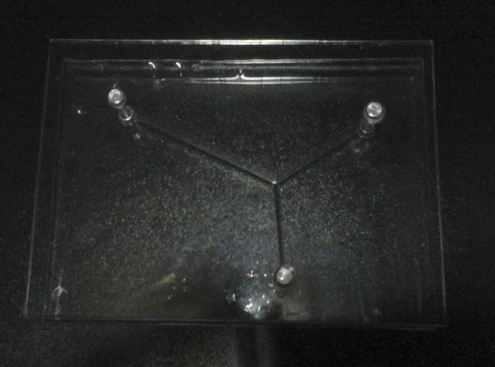
\includegraphics[scale=0.35]{steiner1}
	}\hspace{0.75cm}
	\subfloat{
		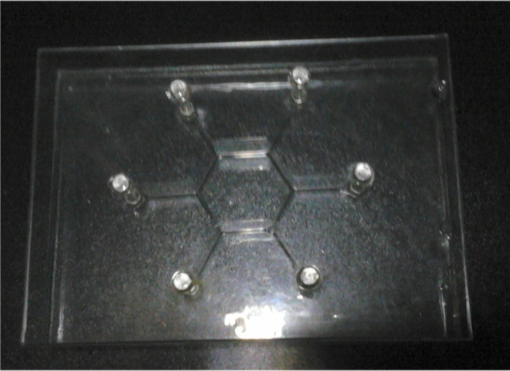
\includegraphics[scale=0.35]{steiner3}
	}\\\vspace{.5cm}
	\subfloat{
		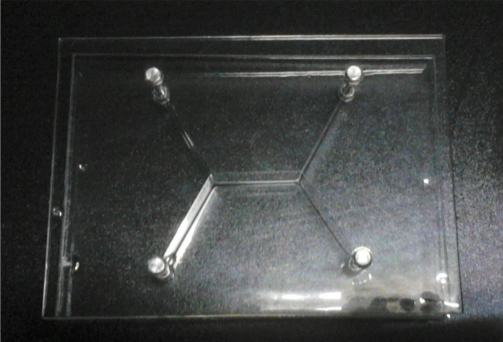
\includegraphics[scale=0.38]{steiner2}
	}
	\
	
	\caption[]{Arbres de Steiner amb bombolles de sabó\footnotemark}
	\label{fig:Steiner}	
\end{figure}
\footnotetext{Autor: Anton Aubanell}

\section{Arbres expansius}
Quan hi ha una situació on no es pot afegir cap node, el millor sol ser utilitzar els algorismes per trobar arbres expansius que ja s'han vist. Una opció és construir el graf complet amb totes les arestes i els seus corresponents pesos i executar algun algorisme que en trobi l'arbre expansiu mínim. 
\\

\newpage
\chapter{Aplicacions pràctiques de la teoria de grafs}

\section{Algorisme PageRank}
Una de les aplicacions de teoria de grafs que utilitzem cada dia és l'algorisme PageRank de Google. A través d'aquest algorisme, el cercador pot saber quines pàgines web són més valorades per la comunitat d'usuaris en general i, per tant, en quin ordre s'han de presentar els resultats d'una cerca.

Una versió simpificada d'aquest algorisme (l'utilitzat actualment és molt complex i s'escapa de la comprensió de l'autor) compta el nombre de links que s'adrecen a la pàgina web, així com la importància de les pàgines web on estan posats aquests enllaços, per saber quina importància té una web. La presuposició que fan és que quans més links cap a una web concreta i més important és la web d'origen, més important és la web de destí.

S'ha de pensar el conjunt de pàgines web com un graf dirigit i ponderat: cada vèrtex representa una pàgina i hi ha una aresta dirigida des del vèrtex $v_{i}$ fins a $v_{j}$ si hi ha un enllaç a $v_{i}$ que porta a $v_{j}$. El pes de l'aresta $e=(v_{i}, v_{j})$, $w(e)$, serà la probabilitat de passar del vèrtex $v_{i}$ al vèrtex $v_{j}$ (és a dir, $\frac{1}{n}$, on $n$ és el nombre d'arestes que surten de $v_{i}$).

Un cop es té la matriu de probabilitats (la matriu d'adjacència del graf) es fa que un programa o bot navegui de manera aleatòria per aquest graf, d'acord amb les probabilitats de passar per cada aresta. Quan el programa ha estat un temps recorrent els nodes del graf es fa el recompte de quantes vegades ha passat per a cada pàgina, i a partir d'aquest valor es determina la posició en els resultats.

\section{Comerç online: productes relacionats}
Quan es visita una botiga online i s'està mirant un producte, sovint apareix una secció de productes recomenats o relacionats. Hi ha diverses maneres de saber quins productes estan relacionats amb aquell que s'està mirant, i una de les que més s'utilitza es basa en teoria de grafs. 

El que es fa és anar construïnt un graf a mesura que els usuaris van visitant la web: cada producte és un vèrtex, i es genera una aresta dirigida cap a un altre producte quan aquest és visitat immediatament després del primer. Per exemple, si un usuari busca un ordinador portàtil, el més probable és que a l'acabar de mirar-ne un en visiti un altre. En aques cas es generaria una aresta des del primer ordinador fins al segon. A mesura que els usuaris van utilitzant la web, es van generant arestes i el graf va creixent. Tot i això, és possible que l'usuari, a l'acabar de mirar l'ordinador es posi a buscar un altre article que no hi té res a veure, com per exemple un paraigües. Però això no és habitual, i hi haurà molt poques arestes que uneixin l'ordinador i el paraigües.

Sobre aquest graf s'executarà un algorisme de clusterització, que buscarà parts del graf que siguin més denses o altament connexes. Aquestes parts segurament seran d'una temàtica concreta, com per exemple el grup dels ordinadors i hi haurà molt poques arestes que surtin d'un grup cap a un altre. Així doncs, els productes relacionats seran aquells que es trobin dins del mateix clúster.


\section{Instal·lació de càmeres de videovigilància}
Un altre exemple és la optimització de sistemes de videovigilància. Amb teoria de grafs es pot saber quin és el mínim nombre de càmeres necessàries per poder vigilar un local, tingui la forma que tingui. Aquest problema és conegut com el problema de la galeria d'art

La intuició diu que, per una sala poligonal amb $n$ vértexs, es pot posar una càmera a cada cantonada (que resulta un total de $n$ càmeres) o de manera més òptima, posant una càmera cada dos vèrtexs (que comporta tenir $\frac{n}{2}$ càmeres). Tot i això, Václav Chvátal afirma en el seu teorema que sempre se n'hauran d'utilitzar com a màxim la part entera de $\frac{n}{3}$.

\subsection{Demostració i procediment}
La resolució d'aquest problema es basa en el fet que qualsevol polígon pot ser descompost en triangles, i més concretament que sempre es pot traçar una corda en el polígon.
Per demostrar-ho, s'agafa un vértex $v$ qualsevol del polígon. Poden passar dues coses:
\begin{itemize}
\item La corda que formen els vèrtexs adjacents a $v$, que anomenarem $u$ i $w$, està completament dins el polígon. En aquest cas es pot traçar la corda sense problemes.

\begin{figure}[H]
\centering
	\begin{tikzpicture}[point/.style={circle, draw=black, fill=black, thin, minimum size=1mm}, transform shape, scale=.8]
	\node[point, label={$u$}] (u) at (0,0){};
	\node[point, label={$v$}] (v) at (1.5,2.5){};
	\node[point, label={$w$}] (w) at (3,0){};
	\draw (u) edge (v);
	\draw (w) edge (v);
	\draw (u) edge[dashed] (w);
	\end{tikzpicture}
\end{figure}

\item El propi polígon creua la corda entre $u$ i $w$ . Això voldrà dir que a l'espai delimitat pel triangle que formaríen $v$,$u$ i $w$ hi haurà com a mínim un altre vèrtex del polígon. En aquest cas també es podran traçar diverses cordes amb aquest vàrtex i triangular d'una altra manera.

\begin{figure}[H]
\centering
	\begin{tikzpicture}[point/.style={circle, draw=black, fill=black, thin, minimum size=1mm}, invisible/.style={shape=coordinate}, transform shape, scale=.8]
	\node[point, label={$u$}] (u) at (0,0){};
	\node[point, label={$v$}] (v) at (1.5,2.5){};
	\node[point, label={$w$}] (w) at (3,0){};
	\node[point] (i) at (1.5,1.25){};
	\node[invisible] (j) at (0.75,-0.25){};
	\node[invisible] (k) at (2.25,-0.25){};
	\draw (u) edge (v);
	\draw (w) edge (v);
	\draw (u) edge[dashed, color=red] (w);
	\draw (j) edge (i);
	\draw (k) edge (i);
	\draw (i) edge[dashed] (v);
	\draw (i) edge[dashed] (u);
	\draw (i) edge[dashed] (w);
	\end{tikzpicture}
\end{figure}
\end{itemize}

Si s'agafa el polígon triangulat com a graf (on els vèrtexs del polígon són els nodes i els costats i cordes són les arestes), els vèrtexs d'aquest poden ser pintats mitjançant tres colors, de tal manera que cada triangle tingui un vèrtex de cada color (d'aquí l'aproximació de $\frac{n}{3}$). Qualsevol conjunt de vèrtex d'un mateix color és un conjunt de posicions vàlides per a les càmeres de seguretat. Tan sols cal veure quin és el conjunt de menys elements per poder determinar les posicions vàlides de les càmeres. 

Cal puntualitzar que hi ha casos on amb aquest procediment no es troba la solució òptima al problema, és tan sols una bona aproximació.

\begin{figure}[H]
\definecolor{qqqqff}{rgb}{0,0,1}
\definecolor{fftttt}{rgb}{1,0.2,0.2}
\definecolor{qqffqq}{rgb}{0,1,0}

\subfloat[]{
\begin{tikzpicture}[line cap=round,line join=round,>=triangle 45,x=1.0cm,y=1.0cm]
	\clip(0.61,-0.09) rectangle (5.12,5.1);
	\draw [line width=1.2pt] (0.58,0.9)-- (3.08,0.74);
	\draw [line width=1.2pt] (2.76,1.61)-- (3.08,0.74);
	\draw [line width=1.2pt] (2.76,1.61)-- (5,1.42);
	\draw [line width=1.2pt] (5,1.42)-- (3.79,3.27);
	\draw [line width=1.2pt] (3.79,3.27)-- (4.67,2.74);
	\draw [line width=1.2pt] (4.67,2.74)-- (5.01,4.55);
	\draw [line width=1.2pt] (5.01,4.55)-- (2.82,3.38);
	\draw [line width=1.2pt] (2.82,3.38)-- (2.22,4.38);
	\draw [line width=1.2pt] (2.22,4.38)-- (1.23,3.13);
	\draw [line width=1.2pt] (0.58,0.9)-- (3.47,2.63);
	\draw [line width=1.2pt] (1.23,3.13)-- (3.47,2.63);
\end{tikzpicture}
}
\subfloat[]{
\centering
\begin{tikzpicture}[line cap=round,line join=round,>=triangle 45,x=1.0cm,y=1.0cm]
	\clip(0.61,-0.09) rectangle (5.12,5.1);
	\draw [line width=1.2pt] (0.58,0.9)-- (3.08,0.74);
	\draw [line width=1.2pt] (2.76,1.61)-- (3.08,0.74);
	\draw [line width=1.2pt] (2.76,1.61)-- (5,1.42);
	\draw [line width=1.2pt] (5,1.42)-- (3.79,3.27);
	\draw [line width=1.2pt] (3.79,3.27)-- (4.67,2.74);
	\draw [line width=1.2pt] (4.67,2.74)-- (5.01,4.55);
	\draw [line width=1.2pt] (5.01,4.55)-- (2.82,3.38);
	\draw [line width=1.2pt] (2.82,3.38)-- (2.22,4.38);
	\draw [line width=1.2pt] (2.22,4.38)-- (1.23,3.13);
	\draw [line width=1.2pt] (0.58,0.9)-- (3.47,2.63);
	\draw [line width=1.2pt] (1.23,3.13)-- (3.47,2.63);
	\draw [dash pattern=on 1pt off 1pt] (1.23,3.13)-- (2.82,3.38);
	\draw [dash pattern=on 1pt off 1pt] (2.82,3.38)-- (3.47,2.63);
	\draw [dash pattern=on 1pt off 1pt] (3.47,2.63)-- (3.79,3.27);
	\draw [dash pattern=on 1pt off 1pt] (2.82,3.38)-- (3.79,3.27);
	\draw [dash pattern=on 1pt off 1pt] (3.79,3.27)-- (5.01,4.55);
	\draw [dash pattern=on 1pt off 1pt] (3.47,2.63)-- (5,1.42);
	\draw [dash pattern=on 1pt off 1pt] (2.76,1.61)-- (3.47,2.63);
	\draw [dash pattern=on 1pt off 1pt] (2.76,1.61)-- (0.58,0.9);
\end{tikzpicture}
}
\subfloat[]{
\centering
\begin{tikzpicture}[line cap=round,line join=round,>=triangle 45,x=1.0cm,y=1.0cm]
	\clip(0.56,-0.09) rectangle (5.12,5.1);
	\draw [line width=1.2pt] (0.58,0.9)-- (3.08,0.74);
	\draw [line width=1.2pt] (2.76,1.61)-- (3.08,0.74);
	\draw [line width=1.2pt] (2.76,1.61)-- (5,1.42);
	\draw [line width=1.2pt] (5,1.42)-- (3.79,3.27);
	\draw [line width=1.2pt] (3.79,3.27)-- (4.67,2.74);
	\draw [line width=1.2pt] (4.67,2.74)-- (5.01,4.55);
	\draw [line width=1.2pt] (5.01,4.55)-- (2.82,3.38);
	\draw [line width=1.2pt] (2.82,3.38)-- (2.22,4.38);
	\draw [line width=1.2pt] (2.22,4.38)-- (1.23,3.13);
	\draw [line width=1.2pt] (0.58,0.9)-- (3.47,2.63);
	\draw [line width=1.2pt] (1.23,3.13)-- (3.47,2.63);
	\draw [dash pattern=on 1pt off 1pt] (1.23,3.13)-- (2.82,3.38);
	\draw [dash pattern=on 1pt off 1pt] (2.82,3.38)-- (3.47,2.63);
	\draw [dash pattern=on 1pt off 1pt] (3.47,2.63)-- (3.79,3.27);
	\draw [dash pattern=on 1pt off 1pt] (2.82,3.38)-- (3.79,3.27);
	\draw [dash pattern=on 1pt off 1pt] (3.79,3.27)-- (5.01,4.55);
	\draw [dash pattern=on 1pt off 1pt] (3.47,2.63)-- (5,1.42);
	\draw [dash pattern=on 1pt off 1pt] (2.76,1.61)-- (3.47,2.63);
	\draw [dash pattern=on 1pt off 1pt] (2.76,1.61)-- (0.58,0.9);

	\begin{scriptsize}
		\fill [color=qqffqq] (0.58,0.9) circle (2.5pt);
		\fill [color=fftttt] (1.23,3.13) circle (2.5pt);
		\fill [color=qqffqq] (4.67,2.74) circle (2.5pt);
		\fill [color=qqqqff] (5.01,4.55) circle (2.5pt);
		\fill [color=qqqqff] (2.22,4.38) circle (2.5pt);
		\fill [color=qqffqq] (2.82,3.38) circle (2.5pt);
		\fill [color=fftttt] (3.79,3.27) circle (2.5pt);
		\fill [color=fftttt] (2.76,1.61) circle (2.5pt);
		\fill [color=qqffqq] (5,1.42) circle (2.5pt);
		\fill [color=qqqqff] (3.08,0.74) circle (2.5pt);
		\fill [color=qqqqff] (3.47,2.63) circle (2.5pt);
	\end{scriptsize}
\end{tikzpicture}
}
\caption{Exemple del procés de triangulació i coloració d'un polígon irregular}
\end{figure}


\section{Xarxa de metro}
Una xarxa de metro és un altre bon exemple de graf: es pot pensar com un conjunt de grafs elementals $P_{n}$ (equivalents a les diverses línies) amb la propietat que alguns d'aquests comparteixen nodes. Així doncs, com a una última aplicació pràctica, em vaig proposar fer un programa que sigués capaç de calcular un trajecte entre dues estacions qualssevol i el temps aproximat de recorregut que es trigaria, incloent-hi els possibles transbords entre línies. 

\subsection{Metodologia de treball}

El primer gran repte consistia a representar l'àmplia xarxa de metro de Barcelona en forma de graf. Cada estació correspon a un node i dos nodes seran adjacents si i només si les estacions estan connectades, ja sigui a través del propi metro o a través de passadissos (cas que tan sols apareix quan diverses línies comparteixen estació). Això comporta representar totes les adjacències de cadascuna de les estacions. Per fer-ho, vàrem dividir la xarxa total en cadascuna de les línies. Per poder tenir en compte els temps de transbord entre línitrgantes d'una mateixa estació, es va crear una estació diferent per a cada línia, unides per una aresta de pes proporcional al temps de transbord. 

Un cop l'adjacència del graf va estar completa, calia posar pesos a cadascuna de les arestes, corresponents al temps de viatge entre estacions mitjançant el metro o, en cas dels transbords, el temps caminant entre les andanes. Per aconseguir aquests temps, es va anar un dia a recòrrer la xarxa sencera, tot cronometrant els intervals de temps necessaris. Tots els temps van ser introduïts al graf en segons, per tal de facilitar el posterior càlcul del temps total.

\subsection{Consideracions}

Cal remarcar que els temps introduits al graf són els temps que va trigar el metro el duimenge 30 d'octubre de 2016, i que aquests no són constants, sinó que poden variar en funció del dia, l'hora i molts altres factors imprevisibles. El mateix passa amb el temps de les parades. Es va observar que el temps que el metro estava parat en una estació s'incrementava en intervals de 5 segons en estacions concretes i a mesura que s'anava apropant al centre de la ciutat. Com que és un factor que també varia en funció de molts paràmetres i massa complex per tenir-lo en compte, s'ha establert que el temps de parada és d'uns 25 segons de mitjana. 

Aquest temps, en un principi, s'afegeigia al total multiplicat pel nombre de parades menys dues (la inicial i la final), però es va observar que aquest procediment no era del tot correcte. Per tal de veure el problema, considerem el següent graf:

\begin{figure}[H]
  \centering
  \begin{tikzpicture}[round/.style={circle, draw=black, thin, minimum size=.5mm}, transform shape, scale=0.8]
    \node[round](0) at (0,0){$v_{0}$};
    \node[round](1) at (2,0){$v_{1}$};
    \node[round](2) at (4,0){$v_{2}$};
    \node[round](3) at (6,0){$v_{3}$};
    \node[round](4) at (8,0){$v_{4}$};
    \node[round](5) at (10,0){$v_{5}$};

    \Edge[label=$1$](0)(1)
    \Edge[label=$1$](1)(2)
    \Edge[label=$1$](2)(3)
    \Edge[label=$1$](3)(4)
    \Edge[label=$1$](4)(5)

    \tikzset{EdgeStyle/.style={bend right=25}} %Arestes múltiples
    \Edge[label=$6$](0)(5)


  \end{tikzpicture}
  \caption{Exemple abstracte de xarxa de metro}
  \label{fig:no_metro}
\end{figure}

En aquest graf, el camí mínim per anar de $v_0$ a $v_5$ segons Dijkstra és passant per la resta de nodes. Posteriorment l'algorisme del metro afegiria els 25 segons multiplicat pel nombre de parades menys una, afegint llavors 125 segons. El resultat total és de 130 segons. Ṕerò el camí mínim no és aquest: si no s'utilitza Dijkstra i s'agafa l'aresta directa entre $v_0$ i $v_5$ s'obté un temps de 6 segons al que només cal sumar 25 segons, trigant un total de 31 segons. Així doncs, l'algorisme era incorrecte, ja que també cal tenir en compte el nombre de nodes per on es passa. Aquest error es pot sol·lucionar de dues maneres:

\begin{itemize}
\item Sumant el temps de parada a tots els temps de trajectes del graf.
\item Sumant el temps de parada a el pas d'assignació de pes de Dijkstra. 
\end{itemize}

Així doncs, els valors de temps que calculi el programa seràn relatius i aproximats.

El format de les estacions en el graf és el següent:
\[ (\text{número de línia})\_(\text{nom d'estació})\]
Els noms de les estacions estan posats d'acord amb el plànol de la xarxa de metro que proporciona TMB (Veure figura \ref{fig:metro}).

\begin{figure}[H]
	\centering
	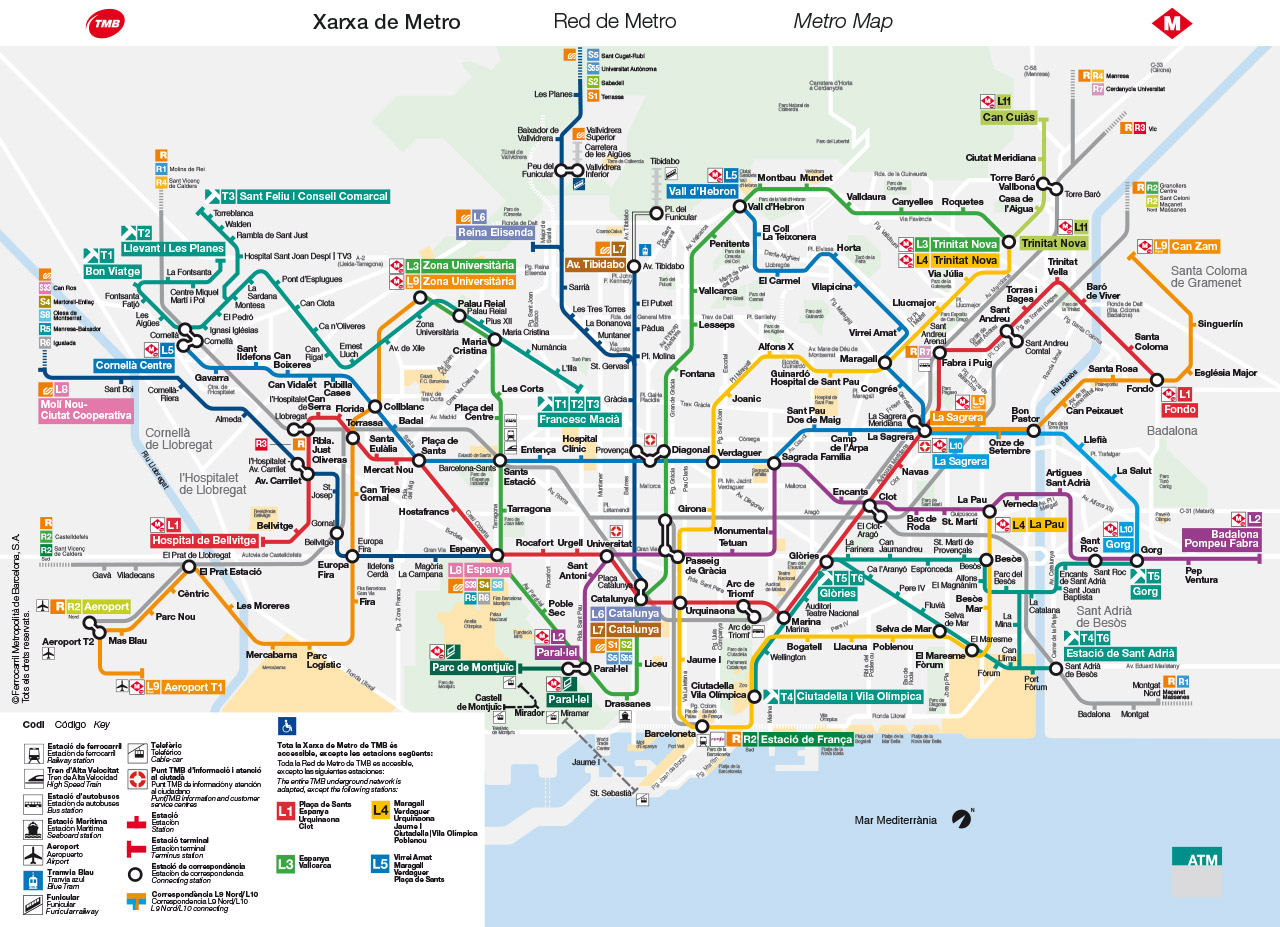
\includegraphics[scale=0.4, angle=90]{metro}
	\caption[]{Plànol de la xarxa de metro de Barcelona \footnotemark}
	\label{fig:metro}	
\end{figure}
\footnotetext{Autor: Ferrocarril Metropolità de Barcelona, S.A. Tots els drets reservats a l'autor}

\subsection{Algorisme}
El programa que fa els càlculs funciona a partir d'una execució de l'algorisme de Dijkstra (en realitat en una versió modificada que pot tractar amb paraules com a noms de nodes).

\begin{algorisme}[H]
\SetKwFunction{DijkstraOrdenat}{DijkstraOrdenat}
\SetKwFunction{FMain}{Programa principal}
\SetKwProg{Fn}{Funció}{}{}
\DontPrintSemicolon
\Fn{\DijkstraOrdenat{$G$, $s$}}
{
nou diccionari $dist$ amb les mateixes claus que $G$\;
nou diccionari $Q$ amb les mateixes claus que $G$\;
nou diccionari $arbre$\;
\ForEach{node $v$ de $G$}
{
	$Q[v]=\infty$\;
	$dist[v]=\infty$\;
}
$Q[s]=0$\;

\While{$Q$ no estigui buit}
{
	$u=min\{\text{valor de } Q\}$\;
	$dist[u]=Q[u]$\;
	\ForEach{node $v$ adjacent a $u$}
	{
		\If{$v$ existeix dins $Q$}
		{
			
			\If{$Q[v]>Q[u]+w(u,v)$}
			{
				$Q[v]=Q[u]+w(u,v)$\;
				$arbre[v] = u$\;
				
			}
		}
	}
	elimina($Q[u]$)\;
}
return $dist$, $arbre$	     
}
\end{algorisme}
\leavevmode
\\
Dijkstra retorna un primer diccionari amb els temps des del node inicial $s$ fins a la resta de nodes i un segon diccionari amb l'arbre expansiu que té $s$ com a arrel. Per saber el recorregut a fer, només cal seguir l'arbre de manera inversa, és a dir des del punt final fins a $s$. Al ser un arbre, només hi haurà un camí possible a seguir.

Per obtenir el temps caldrà buscar l'entrada corresponent al node final al diccionari dels temps. A aquest temps se li afegiran els temps per a cada parada i es farà la conversió de segons a minuts i segons.

\begin{algorisme}[H]
\KwData{Graf $G$ del metro, un node inicial $inici$ i un node final $final$}
\KwResult{Temps total del trajecte, trajecte}
\DontPrintSemicolon
nou vector $recorregut$\;
imprimeix("Punt inicial:", $inici$)\;
imprimeix("Punt final:", $final$)\;

dist, arbre = DijkstraOrdenat($G$, $inici$)\;

$i$ = $final$\;
\While{$arbre[i]$ sigui diferent a $inici$}
{
	afegeix $arbre[i]$ a $recorregut$\;
	$i=arbre[i]$\;
}
afegeix $inici$ a $recorregut$\;
inverteix l'ordre dels elements de $recorregut$\;

$TempsTotal=dist[final]+(25\times (len(recorregut)-2)$\;
$minuts=$ part entera de $TempsTotal/60$\;
$segons=$ (residu de $TempsTotal/60$)$\times 0'60$\;
imprimeix("Temps total del recorregut:", $minuts$, "minuts i", $segons$, "segons")\;
imprimeix("Recorregut:")\;
\For{$i$ in $range(0, len(recorregut))$}
{
	imprimeix($recorregut[i]$)\;
}

\end{algorisme}

El funcionament seria el següent:
\subsubsection*{Exemple d'entrada 1}
\begin{minted}[breaklines=true, frame=lines]{python}
metro(graf_metro, "4_Llucmajor", "9S_Aeroport T1")
\end{minted}
\subsubsection*{Exemple de sortida 1}
\begin{minted}[breaklines=true, frame=lines]{text}
Punt inicial: 4_Llucmajor
Punt final: 9S_Aeroport T1
Temps net del recorregut: 2915
Temps total del recorregut: 59 minuts i 0 segons
Recorregut: [ 4_Llucmajor, 4_Maragall, 4_Guinardó Hospital de Sant Pau, 4_Alfons X, 4_Joanic, 4_Verdaguer, 5_Verdaguer, 5_Diagonal, 5_Hospital Clínic, 5_Entença, 5_Sants Estació, 5_Plaça de Sants, 5_Badal, 5_Collblanc, 9S_Collblanc, 9S_Torrassa, 9S_Can Tries Gornal, 9S_Europa Fira, 9S_Fira, 9S_Parc Logístic, 9S_Mercabarna, 9S_Les Moreres, 9S_El Prat Estació, 9S_Cèntric, 9S_Parc Nou, 9S_Mas Blau, 9S_Aeroport T2, 9S_Aeroport T1 ]
\end{minted}

\subsubsection*{Exemple d'entrada 2}
\begin{minted}[breaklines=true, frame=lines]{python}
metro(graf_metro, "3_Zona Universitària", "5_Sagrada Família")
\end{minted}
\subsubsection*{Exemple de sortida 2}
\begin{minted}[breaklines=true, frame=lines]{text}
Punt inicial: 3_Zona Universitària
Punt final: 5_Sagrada Família
Temps net del recorregut: 920
Temps total del recorregut: 19 minuts i 3 segons
Recorregut: [ 3_Zona Universitària, 3_Palau Reial, 3_Maria Cristina, 3_Les Corts, 3_Plaça del Centre, 3_Sants Estació, 5_Sants Estació, 5_Entença, 5_Hospital Clínic, 5_Diagonal, 5_Verdaguer, 5_Sagrada Família ]
\end{minted}

\newpage
\chapter{Conclusions}

Durant aquest treball hem fet un camí juntament amb la teoria de grafs: l'hem vist néixer del pensament d'Euler; l'hem vist créixer acompanyada d'alguns dels més grans matemàtics de l'història; n'hem vist la seva manera d'entendre i modelitzar el món; l'hem acompanyada fins a la seva maduresa on, juntament amb més matemàtics i teòrics de les ciències de computació, ha col·laborat amb una infinitat d'àrees que en un principi semblaven distants a ella; i finalment ens ha ajudat a resoldre problemes quotidians.

Càmeres de vigilància, navegadors GPS, xarxes socials, xarxes telemàtiques, xarxes elàctriques, planificació d'horaris, organització d'un treball, clavagueram... Tots aquest són exemples clars de que lateoria de grafs forma part de la nostra realitat. Verifico, doncs, la meva hipòtesi inicial: la teoria de grafs ofereix aplicacions práctiques a la vida quotidiana. I, com a conclusió, afegiria: difícilment algú pot quedar-ne al marge. 
En la segona part de l'hipòtesi exposava que hi havia mecanismes que permetien fer el pas de la teoria a la realitat. El que és cert és que, com a usuaris, ens queden lluny i difícilment són visibles o apreciables. Aquests mecanismes són els algorismes que, a partir d'unes dades concretes, ofereixen una resolució, una resposta. Al llarg del treball he vist i he demostrat que al darrere d'aquests procediments hi ha matemàtiques, tal com es pretenia validar. Podríem dir que he ampliat es objectius incials al poder comprendre i analitzar el funcionament de tots aquests algorismes i, encara més, al generar-ne de nous. 
Una altra conclusió és que tota la matemàtica vinculada a la teoria de grafs esdevé complexa i requereix, en general, de l'ús dels ordinadors. Així ho van començar a veure Appel i Hanken en la seva demostració del teorema dels quatre colors i així ho he pogut constatar mitjançant programes com el del metro.  


Personalment, el treball m'ha ajudat molt. He après moltíssim de teoria de grafs, però el que és també molt important és el rerefons més abstracte: el tipus de raonament matemàtic, la formalització de conceptes i idees, les tècniques de demostració, la metodologia matemàtica... Amb tot això he pogut descobrir la capacitat modelitzadora de les matemàtiques.
Amb aquest treball també m'he iniciat a la programació en Phyton. En un principi tenia pensat escriure els algorismes en C++, llenguatge que he utilitzat molt més, però vaig decidir intentar-ho fer amb un llenguatge que aportés una visió diferent de la programació a la que tenia dels basats en C. Mitjançant la programació he viscut l'aventura de relacionar i aplicar idees matemàtiques a algorismes i posteriorment "dotar-los de vida" implementant-los en programes.   
També cal afegir-hi l'existència d'un component més emocional. És el camp d'un dels primers "grans" problemes a els quals em vaig enfrontar, i m'ho he passat molt bé aprenent més sobre aquesta branca. 
Tot aqusts coneixemets adquirits em fan veure el món d'una manera lleugerament diferent, i de ben segur que em seràn útils pels meus estudis futurs en el camp de les matemàtiques i la informàtica.

Encara que el treball final no contingui tots els aspectes que m'hagués agradat tractar, el camí que n'ha resultat és fins i tot més ampli del que en un principi podia imaginar. 

Això sí: tot i que el camí sempre ha fet pujada, cal pensar que cada vegada som més aprop del cim.

\newpage

\printbibliography[keyword=refer, title=Referències, resetnumbers=true]%, prefixnumbers=A]
\nocite{*}
\newpage
\printbibliography[env=nolabelbib, keyword=biblio, title=Bibliografia, resetnumbers=true]%, prefixnumbers=B]
%\bibliographystyle{ieeetr}

\newpage

\appendix
\chapter{Programari}
Per poder realitzar aquest treball ha sigut necessari fer un ús extensiu d'eines informàtiques. Penso que és important posar en valor totes aquestes eines utilitzades que, directa o indirectament han afectat en el desenvolupament del treball. Tot el programari que s'ha utliitzat durant el transcurs del treball és programari lliure, de codi obert i gratuït.

\section{Sistemes operatius}
Encara que la majoria de programes utilitzats tenen versions per a altres sistemes operatius, jo els he utilitzat sobre sistemes GNU/Linux, concretament amb distribucions Ubuntu i Debian.

\section{Processador de text}
Per tal de poder redactar el treball ha sigut necessari un processador de textos especial. Ha sigut necessari escriure un gran nombre de fórmules i expressions matemàtiques, pseudocodi, programes complets... i en aquest aspecte \LaTeX  ha ajudat molt. LaTeX és un "sistema de composició de text" amb una "alta qualitat tipogràfica", on en lloc d'escriure el text podríem dir que es programa. D'aquesta manera s'aconsegueix exactament el que es desitja, essent possible modificar tots i cadascun dels paràmetres del document.
Per exemple: 
la fórmula
\[ e'=\frac{1}{2} \sum_{i=1}^{n}g(v_{i})^{2}-e \]
s'escriu a LaTeX com a 
\begin{minted}[breaklines=true]{tex}
\[ e'=\frac{1}{2} \sum_{i=1}^{n}g(v_{i})^{2}-e \]
\end{minted}
Posteriorment, tot el codi es compila i es genera un fitxer .pdf amb tot el codi interpretat.

També permet la utilització de diversos paquets que afegeixen funcionalitats. Durant la redaccó d'aquesta memòria se n'han utilitzat un total de 32. Els següents són els més importants:

\subsection{Tikz i tkz-berge}
La gran majoria de imatges fetes per mi mateix s'han fet a través d'aquests paquets. Inclouen diverses funcions orientades a grafs i permeten dibuixar-los tal com es desitgin. La següent imatge d'un graf 

\begin{figure}[H]
	\centering
	\begin{tikzpicture}[round/.style={circle, draw=black, thin, minimum size=2mm}, transform shape, scale=0.5]
		\node[round,orange] (3) at (0,4) {$v_{3}$};
		\node[round,orange] (4) at (0,0) {$v_{4}$};
		\node[round,orange] (2) at (4,0) {$v_{2}$};
		\node[round,orange] (1) at (4,4) {$v_{1}$};
		\node[round,orange] (0) at (6,2) {$v_{0}$};

		
		\Edge[label=$5$](2)(4)
		\tikzset{EdgeStyle/.style={orange}}
		\Edge[label=$1$](0)(1)
		\Edge[label=$3$](1)(2)
		\Edge[label=$4$](1)(4)
		\Edge[label=$2$](3)(4)

	\end{tikzpicture}
\end{figure}

s'escriu a LaTeX com a 

\begin{minted}[breaklines=true]{tex}
\begin{figure}[H]
	\centering
	\begin{tikzpicture}[round/.style={circle, draw=black, thin, minimum size=2mm}, transform shape, scale=0.5]
		\node[round,orange] (3) at (0,4) {$v_{3}$};
		\node[round,orange] (4) at (0,0) {$v_{4}$};
		\node[round,orange] (2) at (4,0) {$v_{2}$};
		\node[round,orange] (1) at (4,4) {$v_{1}$};
		\node[round,orange] (0) at (6,2) {$v_{0}$};

		
		\Edge[label=$5$](2)(4)
		\tikzset{EdgeStyle/.style={orange}}
		\Edge[label=$1$](0)(1)
		\Edge[label=$3$](1)(2)
		\Edge[label=$4$](1)(4)
		\Edge[label=$2$](3)(4)

	\end{tikzpicture}
\end{figure}

\end{minted}

\subsubsection{Minted i Algorithm2e}
Minted és el paquet que permet introduïr codi amb el seu format corresponent i ressaltant la sintaxi. D'altra banda, algorithm2e és l'encarregat de donar format al pseudocodi.

\subsection{GeoGebra}
GeoGebra és un porgrama muliús, útil tant en el camp de la geometria, com en l'àlgebra o el càlcul. En aquest cas ha estat utilitzat per a generar les imatges dels punts de Fermat i alguna altra figura concreta com el polígon del problema de les càmeres de seguretat.

\subsection{Python} 
Python és un lenguatge de propòsit general i d'alt nivell que busca senzillesa i eficiència fent que la sintaxi sigui més senzilla de llegir. Aquest llenguatge permet escriure programes més entenedors i en menys línies que altres llenguatges com C/C++.

\newpage
\chapter{Algorismes}
\section{DFS}
\subsection{Codi}
\begin{minted}[frame=lines, breaklines=true]{python}
parent={}
topo=[] 
def DFS(Adj):
    node=[]
    for i in range(0, len(Adj)):
        node.append(i)

    for s in node:
        if s not in parent:
            print "From node %d:" %s
            print s            
            parent[s]=None
            DFS_recursive(Adj, s)
    print "Recursion order (topological sort for directed acyclic graphs):"
    topo.reverse()    
    print topo


def DFS_recursive(Adj, s):
    for v in Adj[s]:
        if v not in parent:                
            print v
            parent[v]=s
            DFS_recursive(Adj, v)
    topo.append(s)
\end{minted}
\subsection{Exemple d'entrada}
\begin{minted}[frame=lines, breaklines=true]{python}
G={0:[1,2,3], 1:[3,4], 2:[4], 3:[4], 4:[]}
print DFS(G)
\end{minted}
\subsection{Exemple de sortida}
\begin{minted}[frame=lines, breaklines=true]{text}
Des de 0 es pot arribar a:
0
1
3
4
2
Ordenació topològica:
[0, 2, 1, 3, 4]
\end{minted}

\section{BFS}
\subsection{Codi}
\begin{minted}[frame=lines, breaklines=true]{python}
def BFS(Adj, s):
    level={s:0}
    parent={s:None}
    i=1
    frontier=[s]
    print s
    while frontier:
        next=[]
        for u in frontier:
            for v in Adj[u]:
                if v not in  level:
                    level[v]=i
                    parent[v]=u
                    next.append(v)
                    print v
        frontier=next
        i+=1
    print level
\end{minted}
\ubsection{Exemple d'entrada}
\begin{minted}[frame=lines, breaklines=true]{python}
G={0:[1,2,3], 1:[3,4], 2:[4], 3:[4], 4:[]}
print BFS(G, 0)
\end{minted}
\subsection{Exemple de sortida}
\begin{minted}[frame=lines, breaklines=true]{text}
{0: 0, 1: 1, 2: 1, 3: 1, 4: 2}
\end{minted}


\section{Dijkstra}
\subsection{Codi}
\begin{minted}[frame=lines, breaklines=true]{python}
def Dijkstra(Adj, s):
    Q={}
    dist={}
    tree={}
    for i in range(0, len(Adj)):
        Q[i]=float("inf")
        dist[i]=float("inf")
    Q[s]=0
    while Q:
        u = min(Q, key=Q.get)
        dist[u] = Q[u]
        for v in Adj[u]:
            if v in Q:
                if Q[v] > Q[u] + Adj[u][v]:
                    Q[v] = Q[u] + Adj[u][v]
                    tree[v] = u
        Q.pop(u)
        
    return dist, tree


def OrderedDijkstra(Adj, s):
    Q = dict.fromkeys(Adj.keys(), float("inf"))
    dist = dict.fromkeys(Adj.keys(), float("inf"))
    tree = {}
    Q[s] = 0
    while Q:
        u = min(Q, key=Q.get)
        dist[u] = Q[u]
        for v in Adj[u]:[0, 2, 1, 4, 3, 5]
            if v in Q:
                if Q[v] > Q[u] + Adj[u][v]:
                    Q[v] = Q[u] + Adj[u][v]
                    tree[v] = u
        Q.pop(u)
        
    return dist, tree
\end{minted}
\subsection{Exemple d'entrada}
\begin{minted}[frame=lines, breaklines=true]{python}
G={0:{1:10,2:3},1:{2:1, 3:2},2:{1:4, 3:8, 4:2},3:{4:7},4:{3:9}}
distancies, arbre_anteriors = Dijkstra(G, 0)
print distancies
print arbre_apuntadors
\end{minted}
\subsection{Exemple de sortida}
\begin{minted}[frame=lines, breaklines=true]{text}
{0: 0, 1: 7, 2: 3, 3: 9, 4: 5}
{1: 2, 2: 0, 3: 1, 4: 2}
\end{minted}
\section{Bellman-Ford}
\subsection{Codi}
\begin{minted}[frame=lines, breaklines=true]{python}
def BellmanFord(Adj, s):
    dist={}
    tree={}
    for i in range(0, len(Adj)):
        dist[i]=float("inf")
        tree[i]=None
    dist[s]=0
    
    for i in range(0, len(Adj)-1):
        for u in range(0, len(Adj)):
            for v in Adj[u]:
                if dist[v] > dist[u] + Adj[u][v]:
                    dist[v] = dist[u] + Adj[u][v]
                    tree[v]=u
    for u in range(0, len(Adj)):
        for v in Adj[u]:
            if dist[v] > dist[u] + Adj[u][v]:
                print "There are negative-weight cycles"
                break
    return dist, tree
\end{minted}
\subsection{Exemple d'entrada}
\begin{minted}[frame=lines, breaklines=true]{python}
G={0:{1:16,2:0}, 1:{2:-32}, 2:{3:8,4:0}, 3:{4:-16}, 4:{5:4,6:0}, 5:{6:-8}, 6:{7:2,8:0}, 7:{8:-4}, 8:{9:1,10:0}, 9:{10:-2},10:{}}
distancies, arbre_apuntadors = BellmanFord(G, 0)
print distancies
print arbre_apuntadors
\end{minted}
\subsection{Exemple de sortida}
\begin{minted}[frame=lines, breaklines=true]{text}
{0: 0, 1: 16, 2: -16, 3: -8, 4: -24, 5: -20, 6: -28, 7: -26, 8: -30, 9: -29, 10: -31}
{0: None, 1: 0, 2: 1, 3: 2, 4: 3, 5: 4, 6: 5, 7: 6, 8: 7, 9: 8, 10: 9}
\end{minted}
\section{Prim}
\subsection{Codi}
\begin{minted}[frame=lines, breaklines=true]{python}
def Prim(Adj):
    Q={}
    tree={}
    for i in range(0,len(Adj)):
        Q[i]=float("inf")
    Q[0]=0
    while Q:
        u = min(Q, key=Q.get)
        for v in Adj[u]:
            if v in Q and Adj[u][v] < Q[v]:
                Q[v] = Adj[u][v]
                tree[v] = u
        Q.pop(u)
    return tree
\end{minted}
\subsection{Exemple d'entrada}
\begin{minted}[frame=lines, breaklines=true]{python}
G={1:{2:1, 3:2},0:{1:10,2:3},2:{1:4, 3:8, 4:2},4:{3:9},3:{4:7}}
print Prim(G)
\end{minted}
\subsection{Exemple de sortida}
\begin{minted}[frame=lines, breaklines=true]{text}
{1: 2, 2: 0, 3: 1, 4: 2}
\end{minted}

\section{Kruskal}
\subsection{Codi}
\begin{minted}[frame=lines, breaklines=true]{python}
def Kruskal(Adj):
    subtree = UnionFind()
    tree = [] 
    for e, u, v in sorted((Adj[u][v],u,v) for u in Adj for v in Adj[u]):
        for u in Adj:
            for v in Adj[u]:
                if subtree[u] != subtree[v]:
                    tree.append((u,v))
                    subtree.union(u,v)
    return tree
\end{minted}
\subsection{Exemple d'entrada}
\begin{minted}[frame=lines, breaklines=true]{python}
G={0:{1:8,3:2},1:{0:8,2:5,3:3,4:1},2:{1:5,3:2,4:4},3:{0:2,1:3,2:2},4:{1:1,2:4}}
print Prim(G)
\end{minted}
\subsection{Exemple de sortida}
\begin{minted}[frame=lines, breaklines=true]{text}
[(0, 1), (0, 3), (1, 2), (1, 4)]
\end{minted}

\section{Floyd-Warshall}
\begin{minted}[frame=lines, breaklines=true]{python}
def FloydWarshall(Adj):
    dist=[[float("inf") for x in range(len(Adj))] for y in range(len(Adj))]
    for i in range(0,len(Adj)):
       dist[i][i] = 0
    for v in range(len(Adj)):
        for u in Adj[v]:
            dist[v][u] = Adj[v][u]
    for x in range(len(Adj)):
        for u in range(len(Adj)):
            for v in range(len(Adj)):
                if dist[u][v] > dist[u][x] + dist[x][v]:
                    dist[u][v] = dist[u][x] + dist[x][v]
    return dist
\end{minted}
\subsection{Exemple d'entrada}
\begin{minted}[frame=lines, breaklines=true]{python}
G={0:{1:10,2:3},1:{2:1, 3:2},2:{1:4, 3:8, 4:2},3:{4:7},4:{3:9}}
print FloydWarshall(G)
\end{minted}
\subsection{Exemple de sortida}
\begin{minted}[frame=lines, breaklines=true]{text}
[[0, 7, 3, 9, 5], 
[inf, 0, 1, 2, 3], 
[inf, 4, 0, 6, 2], 
[inf, inf, inf, 0, 7], 
[inf, inf, inf, 9, 0]]
\end{minted}


\section{Hamilton}
\subsection{Codi}
\begin{minted}[frame=lines, breaklines=true]{python}
def Hamilton_recursive(Adj, s, e, path):
    path = path + [s]
    if s == e:
        return path
    for n in Adj[s]:
        if n not in path:
            nou_path = Hamilton_recursive(Adj, n, e, path)
            if nou_path: 
                return nou_path
    return None
    
def Hamilton(Adj, s, e):
    path=[]
    return Hamilton_recursive(Adj, s, e, path)
\end{minted}
\subsubsection{Exemple d'entrada}
\begin{minted}[frame=lines, breaklines=true]{python}
G={0:[2,3,5,1],1:[0,2,4,5],2:[0,1,3,4],3:[0,2,4,5],4:[1,2,3,5],5:[0,1,3,4]}
print Hamilton(G, 0, 5)
\end{minted}
\subsection{Exemple de sortida}
\begin{minted}[frame=lines, breaklines=true]{text}
[0, 2, 1, 4, 3, 5]
\end{minted}

\section{Euler}
\subsection{Codi}
\begin{minted}[frame=lines, breaklines=true]{python}
def Euler(Adj):
    graf = Adj
    senar = [v for v in graf.keys() if len(graf[v])%2 != 0]
    senar.append(graf.keys()[0])
    print senar
    
    if len(senar)>3:
        return None
        
    Q = [senar[0]]
    path = []
    while Q:
        v = Q[-1]
        if graf[v]:
            u = graf[v][0]
            Q.append(u)
            del graf[u][graf[u].index(v)]
            del graf[v][0]
        else:
            path.append(Q.pop())
            
    return path
\end{minted}
\subsection{Exemple d'entrada}
\begin{minted}[frame=lines, breaklines=true]{python}
G={0:[1,2,3],1:[0,2,3],2:[0,1,3,4],3:[0,1,2,4],4:[3,2]}
print Euler(G)
\end{minted}
\subsection{Exemple de sortida}
\begin{minted}[frame=lines, breaklines=true]{text}
[1, 3, 4, 2, 3, 0, 2, 1, 0]
\end{minted}


\section{Coloració}
\subsection{Codi}
\begin{minted}[frame=lines, breaklines=true]{python}
def coloring(Adj):
    graph = sorted(Adj, key=lambda k:len(Adj[k]), reverse=True)
    colors = {}
    usat = False
    actual = 0
    
    for i in range(0, len(Adj)):
        colors[i]=None
    colors[graph[0]]=0
    
    while None in colors.values():     
        for v in graph:
            if colors[v] == None:
                for k in Adj[v]:
                    if colors[k] == actual:
                        usat = True
                        break
                    
                if usat == False:
                    colors[v] = actual
                usat = False
        actual = actual + 1
    return colors
\end{minted}
\subsection{Exemple d'entrada}
\begin{minted}[frame=lines, breaklines=true]{python}
bipartite={0:[4,5,6,7], 1:[4,5,6,7], 2:[4,5,6,7], 3:[4,5,6,7], 4:[0,1,2,3], 5:[0,1,2,3], 6:[0,1,2,3], 7:[0,1,2,3]}
print coloring(bipartite)
\end{minted}
\subsection{Exemple de sortida}
\begin{minted}[frame=lines]{text}
{0: 0, 1: 0, 2: 0, 3: 0, 4: 1, 5: 1, 6: 1, 7: 1}
\end{minted}


\section{Metro}
\subsection{Codi}
\begin{minted}[frame=lines]{python}
def metro(Adj, inici, final):
    recorregut=[]
    
    print "Punt inicial:", inici.decode("ISO-8859-15")
    
    print "Punt final:", final.decode("ISO-8859-15")
    
    dist, tree = OrderedDijkstra(Adj, inici)
    print type(inici)
    print type(final)

    i = final    
    while tree[i] != inici:
        recorregut.append(tree[i])
        i = tree[i]
    
    recorregut.append(inici)        
    recorregut.reverse()

    total= dist[final]+(25*(len(recorregut)-2))
        
    minuts = total/60
    segons = (total%60)*0.60
    print "Temps net del recorregut:", dist[final]
    print "Temps total del recorregut:", int(minuts),"minuts i", int(segons), "segons"

    print "Recorregut:",   
    print "[",
    for i in range(0,len(recorregut)):
        print recorregut[i].decode("ISO-8859-15")+",",

    print final.decode("ISO-8859-15"),"]"    
\end{minted}
\subsection{Exemple d'entrada}
\begin{minted}[breaklines=true, mathescape, frame=lines]{python}
graf_metro={"1_Hospital de Bellvitge":{"1_Bellvitge":90}, "1_Bellvitge":{"1_Hospital de Bellvitge":90, "1_Av. Carrilet":100},"1_Av. Carrilet":{"1_Bellvitge":100, "1_Rbla. Just Oliveras":65, "8_L'Hospitalet - Av. Carrilet":180}, "1_Rbla. Just Oliveras":{"1_Av. Carrilet":65, "1_Can Serra":60}, "1_Can Serra":{"1_Rbla. Just Oliveras":60, "1_Florida":60}, "1_Florida":{"1_Can Serra":60, "1_Torrassa":60}, "1_Torrassa":{"1_Florida":60, "1_Santa Eulàlia":85, "9S_Torrassa":240}, "1_Santa Eulàlia":{"1_Torrassa":85,"1_Mercat Nou":75}, "1_Mercat Nou":{"1_Santa Eulàlia":75, "1_Plaça de Sants":60}, "1_Plaça de Sants":{"1_Mercat Nou":60, "1_Hostafrancs":50, "5_Plaça de Sants":282}, "1_Hostafrancs":{"1_Plaça de Sants:":50, "1_Espanya":55}, "1_Espanya":{"1_Hostafrancs":55, "1_Rocafort":60, "3_Espanya":209, "8_Espanya":120}, "1_Rocafort":{"1_Espanya":60, "1_Urgell":55}, "1_Urgell":{"1_Rocafort":55, "1_Universitat":58}, "1_Universitat":{"1_Urgell":58, "1_Catalunya":50, "2_Universitat":144}, "1_Catalunya":{"1_Universitat":50, "1_Urquinaona":58, "3_Catalunya":180, "6_Catalunya":360, "7_Catalunya":360}, "1_Urquinaona":{"1_Catalunya":58, "1_Arc de Triomf":85, "4_Urquinaona":256}, "1_Arc de Triomf":{"1_Urquinaona":85, "1_Marina":54}, "1_Marina":{"1_Arc de Triomf":54, "1_Glòries":80}, "1_Glòries":{"1_Marina":80, "1_Clot":78}, "1_Clot":{"1_Glòries":78,"1_Navas":65, "2_Clot":120}, "1_Navas":{"1_Clot":65, "1_La Sagrera":80}, "1_La Sagrera":{"1_Navas":80, "1_Fabra i Puig":89, "5_La Sagrera":100, "9N_La Sagrera":178, "10_La Sagrera":178}, "1_Fabra i Puig":{"1_La Sagrera":89, "1_Sant Andreu":101}, "1_Sant Andreu":{"1_Fabra i Puig":101, "1_Torras i Bages":88}, "1_Torras i Bages":{"1_Sant Andreu":88, "1_Trinitat Vella":77}, "1_Trinitat Vella":{"1_Torras i Bages":77, "1_Baró de Viver":60}, "1_Baró de Viver":{"1_Trinitat Vella":60, "1_Santa Coloma":83}, "1_Santa Coloma":{"1_Baró de Viver":83, "1_Fondo":84}, "1_Fondo":{"1_Santa Coloma":84, "9N_Fondo":140}, "2_Paral·lel":{"2_Sant Antoni":80, "3_Paral·lel":83}, "2_Sant Antoni":{"2_Paral·lel":80, "2_Universitat":66}, "2_Universitat":{"2_Sant Antoni":66, "2_Passeig de Gràcia":80, "1_Universitat":144}, "2_Passeig de Gràcia":{"2_Universitat":80, "2_Tetuan":95, "3_Passeig de Gràcia":360, "4_Passeig de Gràcia":120}, "2_Tetuan":{"2_Passeig de Gràcia":95, "2_Monumental":93}, "2_Monumental":{"2_Tetuan":93, "2_Sagrada Família":63}, "2_Sagrada Família":{"2_Monumental":63, "2_Encants":114, "5_Sagrada Família":178}, "2_Encants":{"2_Sagrada Família":114, "2_Clot":53}, "2_Clot":{"2_Encants":53, "2_Bac de Roda":89, "1_Clot":120}, "2_Bac de Roda":{"2_Clot":89, "2_Sant Martí":61}, "2_Sant Martí":{"2_Bac de Roda":61, "2_La Pau":74}, "2_La Pau":{"2_Sant Martí":74, "2_Verneda":76, "4_La Pau":60}, "2_Verneda":{"2_La Pau":76, "2_Artigues Sant Adrià":81}, "2_Artigues Sant Adrià":{"2_Verneda":81, "2_Sant Roc":91}, "2_Sant Roc":{"2_Artigues Sant Adrià":91, "2_Gorg":60}, 

"2_Gorg":{"2_Sant Roc":60, "2_Pep Ventura":58, "10_Gorg":78}, "2_Pep Ventura":{"2_Gorg":58, "2_Badalona Pompeu Fabra":74}, "2_Badalona Pompeu Fabra":{"2_Pep Ventura":74}, "3_Zona Universitària":{"3_Palau Reial":67, "9S_Zona Universitària":265}, "3_Palau Reial":{"3_Zona Universitària":67, "3_Maria Cristina":65}, "3_Maria Cristina":{"3_Palau Reial":65, "3_Les Corts":68}, "3_Les Corts":{"3_Maria Cristina":68, "3_Plaça del Centre":63}, "3_Plaça del Centre":{"3_Les Corts":63, "3_Sants Estació":57},"3_Sants Estació":{"3_Plaça del Centre":57, "3_Tarragona":55, "5_Sants Estació":232},"3_Tarragona":{"3_Sants Estació":55, "3_Espanya":65}, "3_Espanya":{"3_Tarragona":65, "3_Poble Sec":67, "1_Espanya":209, "8_Espanya":360}, "3_Poble Sec":{"3_Espanya":67, "3_Paral·lel":70}, "3_Paral·lel":{"3_Poble Sec":70, "3_Drassanes":72, "2_Paral·lel":83}, "3_Drassanes":{"3_Paral·lel":72, "3_Liceu":75}, "3_Liceu":{"3_Drassanes":75, "3_Catalunya":60}, "3_Catalunya":{"3_Liceu":60, "3_Passeig de Gràcia":70, "1_Catalunya":180, "6_Catalunya":180, "7_Catalunya":180}, "3_Passeig de Gràcia":{"3_Catalunya":70, "3_Diagonal":77, "2_Passig de Gràcia":360, "4_Passeig de Gràcia":238}, "3_Diagonal":{"3_Passeig de Gràcia":77, "3_Fontana":75, "5_Diagonal":217, "6_Provença":360, "7_Provença":360}, "3_Fontana":{"3_Diagonal":75, "3_Lesseps":55}, "3_Lesseps":{"3_Fontana":55, "3_Vallcarca":85}, "3_Vallcarca":{"3_Lesseps":85, "3_Penitents":90}, "3_Penitents":{"3_Vallcarca":90, "3_Vall d'Hebron":80}, "3_Vall d'Hebron":{"3_Penitents":80, "3_Montbau":62, "5_Vall d'Hebron":204}, "3_Montbau":{"3_Vall d'Hebron":62, "3_Mundet":64}, "3_Mundet":{"3_Montbau":64, "3_Valldaura":78}, "3_Valldaura":{"3_Mundet":78, "3_Canyelles":79}, "3_Canyelles":{"3_Valldaura":79, "3_Roquetes":94}, "3_Roquetes":{"3_Canyelles":94, "3_Trinitat Nova":84}, "3_Trinitat Nova":{"3_Roquetes":84, "4_Trinitat Nova":210, "11_Trinitat Nova":210}, "4_Trinitat Nova":{"4_Via Júlia":99, "3_Trinitat Nova":210, "11_Trinitat Nova":0}, "4_Via Júlia":{"4_Trinitat Nova":99, "4_Llucmajor":87}, "4_Llucmajor":{"4_Via Júlia":87, "4_Maragall":161}, "4_Maragall":{"4_Llucmajor":161, "4_Guinardó Hospital de Sant Pau":88, "5_Maragall":191}, "4_Guinardó Hospital de Sant Pau":{"4_Maragall":88, "4_Alfons X":86}, "4_Alfons X":{"4_Guinardó Hospital de Sant Pau":86, "4_Joanic":77}, "4_Joanic":{"4_Alfons X":77, "4_Verdaguer":89}, "4_Verdaguer":{"4_Joanic":89, "4_Girona":86, "5_Verdaguer":218}, "4_Girona":{"4_Verdaguer":86, "4_Passeig de Gràcia":83}, "4_Passeig de Gràcia":{"4_Girona":83, "4_Urquinaona":92, "2_Passeig de Gràcia":120, "3_Passeig de Gràcia":238}, "4_Urquinaona":{"4_Passeig de Gràcia":92, "4_Jaume I":60, "1_Urquinaona":256}, "4_Jaume I":{"4_Urquinaona":60, "4_Barceloneta":78}, "4_Barceloneta":{"4_Jaume I":78, "4_Ciutadella Vila Olímpica":82}, "4_Ciutadella Vila Olímpica":{"4_Barceloneta":82, "4_Bogatell":113}, "4_Bogatell":{"4_Ciutadella Vila Olímpica":113, "4_Llacuna":62}, "4_Llacuna":{"4_Bogatell":62, "4_Poblenou":64}, "4_Poblenou":{"4_Llacuna":64, "4_Selva del Mar":66}, "4_Selva del Mar":{"4_Poblenou":66, "4_El Maresme Fòrum":86}, "4_El Maresme Fòrum":{"4_Selva del Mar":86, "4_Besòs Mar":65},

"4_Besòs Mar":{"4_El Maresme Fòrum":65, "4_Besòs":67}, "4_Besòs":{"4_Besòs Mar":67, "4_La Pau":76}, "4_La Pau":{"4_Besòs":76, "2_La Pau":60}, "5_Cornellà Centre":{"5_Gavarra":90}, "5_Gavarra":{"5_Cornellà Centre":90, "5_Sant Ildefons":85}, "5_Sant Ildefons":{"5_Gavarra":85, "5_Can Boixeres":74}, "5_Can Boixeres":{"5_Sant Ildefons":74, "5_Can Vidalet":90}, "5_Can Vidalet":{"5_Can Boixeres":90, "5_Pubilla Cases":83}, "5_Pubilla Cases":{"5_Can Vidalet":83, "5_Collblanc":105}, "5_Collblanc":{"5_Pubilla Cases":105, "5_Badal":70, "9S_Collblanc":240}, "5_Badal":{"5_Collblanc":70, "5_Plaça de Sants":74}, "5_Plaça de Sants":{"5_Badal":74, "5_Sants Estació":79, "1_Plaça de Sants":282}, "5_Sants Estació":{"5_Plaça de Sants":79, "5_Entença":73, "3_Sants Estació":232}, "5_Entença":{"5_Sants Estació":73, "5_Hospital Clínic":64}, "5_Hospital Clínic":{"5_Entença":64, "5_Diagonal":78}, "5_Diagonal":{"5_Hospital Clínic":78, "5_Verdaguer":78, "3_Diagonal":217, "6_Provença":180, "7_Provença":180}, "5_Verdaguer":{"5_Diagonal":78, "5_Sagrada Família":75, "4_Verdaguer":218}, "5_Sagrada Família":{"5_Verdaguer":75, "5_Sant Pau Dos de Maig":85, "2_Sagrada Família":178}, "5_Sant Pau Dos de Maig":{"5_Sagrada Família":85, "5_Camp de l'Arpa":63}, "5_Camp de l'Arpa":{"5_Sant Pau Dos de Maig":63, "5_La Sagrera":93}, "5_La Sagrera":{"5_Camp de l'Arpa":93, "5_Congrés":85, "1_La Sagrera":100, "9N_La Sagrera":233, "10_La Sagrera":233}, "5_Congrés":{"5_La Sagrera":85, "5_Maragall":60}, "5_Maragall":{"5_Congrés":60, "5_Virrei Amat":60, "4_Maragall":191}, "5_Virrei Amat":{"5_Maragall":60, "5_Vilapicina":74}, "5_Vilapicina":{"5_Virrei Amat":74, "5_Horta":75}, "5_Horta":{"5_Vilapicina":75, "5_El Carmel":78}, "5_El Carmel":{"5_Horta":78, "5_El Coll La Teixonera":80}, "5_El Coll La Teixonera":{"5_El Carmel":80, "5_Vall d'Hebron":81}, "5_Vall d'Hebron":{"5_El Coll La Teixonera":81, "3_Vall d'Hebron":204}, "6_Catalunya":{"6_Provença":120, "1_Catalunya":360, "3_Catalunya":180, "7_Catalunya":5}, "6_Provença":{"6_Catalunya":120, "6_Gràcia":120, "3_Diagonal":360, "5_Diagonal":180, "7_Provença":5}, "6_Gràcia":{"6_Provença":120, "6_Sant Gervasi":60, "7_Gràcia":5}, "6_Sant Gervasi":{"6_Gràcia":60, "6_Muntaner":120, "7_Plaça Molina":5}, "6_Muntaner":{"6_Sant Gervasi":120, "6_La Bonanova":60}, "6_La Bonanova":{"6_Muntaner":60, "6_Les Tres Torres":120}, "6_Les Tres Torres":{"6_La Bonanova":120, "6_Sarrià":60}, "6_Sarrià":{"6_Les Tres Torres":60, "6_Reina Elisenda":120}, "6_Reina Elisenda":{"6_Sarrià":120},"7_Catalunya":{"7_Provença":120, "1_Catalunya":360,"3_Catalunya":180, "6_Catalunya":5},"7_Provença":{"7_Catalunya":120, "7_Gràcia":120, "3_Diagonal":360, "5_Diagonal":180, "6_Provença":5},"7_Gràcia":{"7_Provença":120,"7_Plaça Molina":60,"6_Gràcia":5},"7_Plaça Molina":{"7_Gràcia":60,"7_Pàdua":120, "6_Sant Gervasi":5},"7_Pàdua":{"7_Plaça Molina":120,"7_El Putxet":60},"7_El Putxet":{"7_Pàdua":60, "7_Av. Tibidabo":60}, "7_Av. Tibidabo":{"7_El Putxet":60}, "8_Espanya":{"8_Magòria La Campana":120, "1_Espanya":120, "3_Espanya":360}, "8_Magòria La Campana":{"8_Espanya":120, "8_Ildefons Cerdà":120}, 

"8_Ildefons Cerdà":{"8_Magòria La Campana":120, "8_Europa Fira":120}, "8_Europa Fira":{"8_Ildefons Cerdà":120, "8_Gornal":120, "9S_Europa Fira":180}, "8_Gornal":{"8_Europa Fira":120, "8_Sant Josep":120}, "8_Sant Josep":{"8_Gornal":120, "8_L'Hospitalet - Av. Carrilet":60}, "8_L'Hospitalet - Av. Carrilet":{"8_Sant Josep":60, "8_Almeda":180, "1_Av. Carrilet":180}, "8_Almeda":{"8_L'Hospitalet - Av. Carrilet":180, "8_Cornellà - Riera":120}, "8_Cornellà - Riera":{"8_Almeda":120, "8_Sant Boi":180}, "8_Sant Boi":{"8_Cornellà - Riera":180, "8_Molí Nou - Ciutat Cooperativa":120}, "8_Molí Nou - Ciutat Cooperativa":{"8_Sant Boi":120}, "9N_La Sagrera":{"9N_Onze de Setembre":116, "1_La Sagrera":178, "5_La Sagrera":233, "10_La Sagrera":5}, "9N_Onze de Setembre":{"9N_La Sagrera":116, "9N_Bon Pastor":115, "10_Onze de Setembre":5}, "9N_Bon Pastor":{"9N_Onze de Setembre":114, "9N_Can Peixauet":125, "10_Bon Pastor":5}, "9N_Can Peixauet":{"9N_Bon Pastor":125, "9N_Santa Rosa":65}, "9N_Santa Rosa":{"9N_Can Peixauet":65, "9N_Fondo":87}, "9N_Fondo":{"9N_Santa Rosa":87, "9N_Esglèsia Major":72, "1_Fondo":140}, "9N_Esglèsia Major":{"9N_Fondo":72, "9N_Singuerlín":76}, "9N_Singuerlín":{"9N_Esglèsia Major":76, "9N_Can Zam":103}, "9N_Can Zam":{"9N_Singuerlín":103}, "9S_Aeroport T1":{"9S_Aeroport T2":240}, "9S_Aeroport T2":{"9S_Aeroport T1":240, "9S_Mas Blau":80}, "9S_Mas Blau":{"9S_Aeroport T2":80, "9S_Parc Nou":120}, "9S_Parc Nou":{"9S_Mas Blau":120, "9S_Cèntric":85}, "9S_Cèntric":{"9S_Parc Nou":85, "9S_El Prat Estació":95}, "9S_El Prat Estació":{"9S_Cèntric":95, "9S_Les Moreres":150}, "9S_Les Moreres":{"9S_El Prat Estació":150, "9S_Mercabarna":100}, "9S_Mercabarna":{"9S_Les Moreres":100, "9S_Parc Logístic":120}, "9S_Parc Logístic":{"9S_Mercabarna":120, "9S_Fira":125}, "9S_Fira":{"9S_Parc Logístic":125, "9S_Europa Fira":70}, "9S_Europa Fira":{"9S_Fira":70, "9S_Can Tries Gornal":70, "8_Europa Fira":180}, "9S_Can Tries Gornal":{"9S_Europa Fira":70, "9S_Torrassa":75}, "9S_Torrassa":{"9S_Can Tries Gornal":75, "9S_Collblanc":110, "1_Torrassa":240}, "9S_Collblanc":{"9S_Torrassa":110, "9S_Zona Universitària":105, "5_Collblanc":240}, "9S_Zona Universitària":{"9S_Collblanc":105, "3_Zona Universitària":265}, "10_La Sagrera":{"10_Onze de Setembre":116, "1_La Sagrera":178, "5_La Sagrera":233, "9N_La Sagrera":5}, "10_Onze de Setembre":{"10_La Sagrera":116, "10_Bon Pastor":115, "9N_Onze de Setembre":5}, "10_Bon Pastor":{"10_Onze de Setembre":115, "10_Llefià":133, "9N_Bon Pastor":5}, "10_Llefià":{"10_Bon Pastor":133, "10_La Salut":59}, "10_La Salut":{"10_Llefià":59, "10_Gorg":111}, "10_Gorg":{"10_La Salut":111, "2_Gorg":78}, "11_Trinitat Nova":{"11_Casa de l'Aigua":43, "3_Trinitat Nova":210, "4_Trinitat Nova":0}, "11_Casa de l'Aigua":{"11_Trinitat Nova":43, "11_Torre Baró Vallbona":111}, "11_Torre Baró Vallbona":{"11_Casa de l'Aigua":111, "11_Ciutat Meridiana":60}, "11_Ciutat Meridiana":{"11_Torre Baró Vallbona":60, "11_Can Cuiàs":45}, "11_Can Cuiàs":{"11_Ciutat Meridiana":45}}

metro(graf_metro, "2_Paral·lel", "11_Casa de l'Aigua")
\end{minted}
\subsection{Exemple de sortida}
\begin{minted}[breaklines=true, frame=lines]{text}
Punt inicial: 2_Paral·lel
Punt final: 11_Casa de l'Aigua
Temps net del recorregut: 1245
Temps total del recorregut: 26 minuts i 6 segons
Recorregut: [ 2_Paral·lel, 2_Sant Antoni, 2_Universitat, 2_Passeig de Gràcia, 4_Passeig de Gràcia, 4_Girona, 4_Verdaguer, 4_Joanic, 4_Alfons X, 4_Guinardó Hospital de Sant Pau, 4_Maragall, 4_Llucmajor, 4_Via Júlia, 4_Trinitat Nova, 11_Trinitat Nova, 11_Casa de l'Aigua ]
\end{minted}



\end{document}
